\documentclass[a4paper,12pt,titlepage]{report}

% Create a simple test if Tex4ht is loaded
% This is used to determine if the book is compiled with TeX4ht or not.
\makeatletter
\@ifpackageloaded{tex4ht}{\def\iftex4ht{\iftrue}}
                         {\def\iftex4ht{\iffalse}}
\makeatother

\usepackage[a4paper,total={6.5in,9in}]{geometry}
\usepackage[skip=0pt plus1pt, indent=0pt]{parskip}
\usepackage{setspace}
\usepackage{relsize}
\iftex4ht
\else
    \usepackage{CrimsonPro}
    \let\oldnormalfont\normalfont
    \def\normalfont{\oldnormalfont\mdseries}
    \usepackage[T1]{fontenc}
\fi
\usepackage[utf8]{inputenc}
\ifdefined\HCode
	\usepackage[xindy,noautomatic]{imakeidx}
\else
	\usepackage[]{imakeidx}
\fi
\usepackage{tex4ebook}
\usepackage{ifthen}
\usepackage{fancyhdr}
\usepackage{titlesec}
\usepackage{contour}
\usepackage[normalem]{ulem}
\usepackage[defaultlines=3,all]{nowidow}
\usepackage{needspace}
\usepackage{lastpage}
\usepackage[nodayofweek]{datetime}
\usepackage{graphicx}
\usepackage{xcolor}
\usepackage[hyperindex=true]{hyperref}

% Adjust PDF hyperlinks
\hypersetup{
    colorlinks=true,
    linkcolor=blue,
    filecolor=magenta,
    urlcolor=cyan,
    pdftitle={KGLW - The Book of Lyrics},
    %pdfpagemode=fullscreen,
    bookmarks=true,
    bookmarksopen=true,
}

% Disable hyphenation
\tolerance=1
\emergencystretch=\maxdimen
\hyphenpenalty=10000
\hbadness=10000

% Avoid single lines on pages (widows/orphans)
\widowpenalty=10000
\clubpenalty=10000

% Remove lettergroups from EPUB index
\providecommand*\lettergroupDefault[1]{}
\providecommand*\lettergroup[1]{}
\providecommand*\indexspace{}

% Make alphabetical song index (using style file)
\makeindex[intoc,name=songs,columns=2,title={Song Index},options={-s thebook.ist}]

% Make word index (using style file)
\makeindex[intoc,columns=2,title={Word Index},options={-s thebook.ist}]

% Setup title page
\title{%
    \Huge%
    \centering%
    \iftex4ht%
        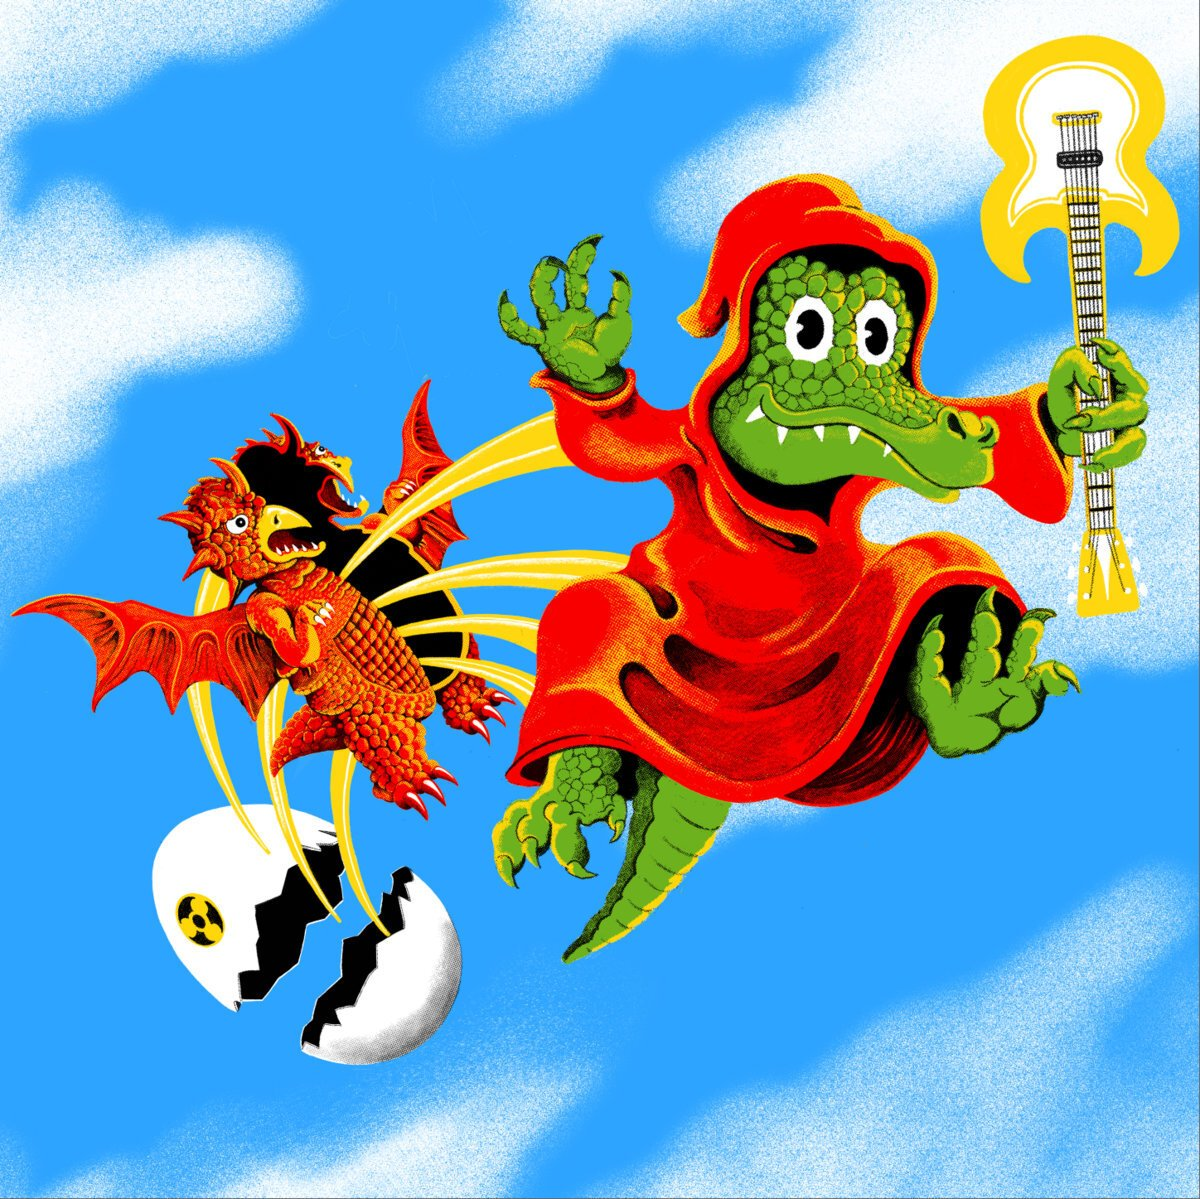
\includegraphics[width=0.6\linewidth]{cover-image.jpg}\\[1em]%
    \else
        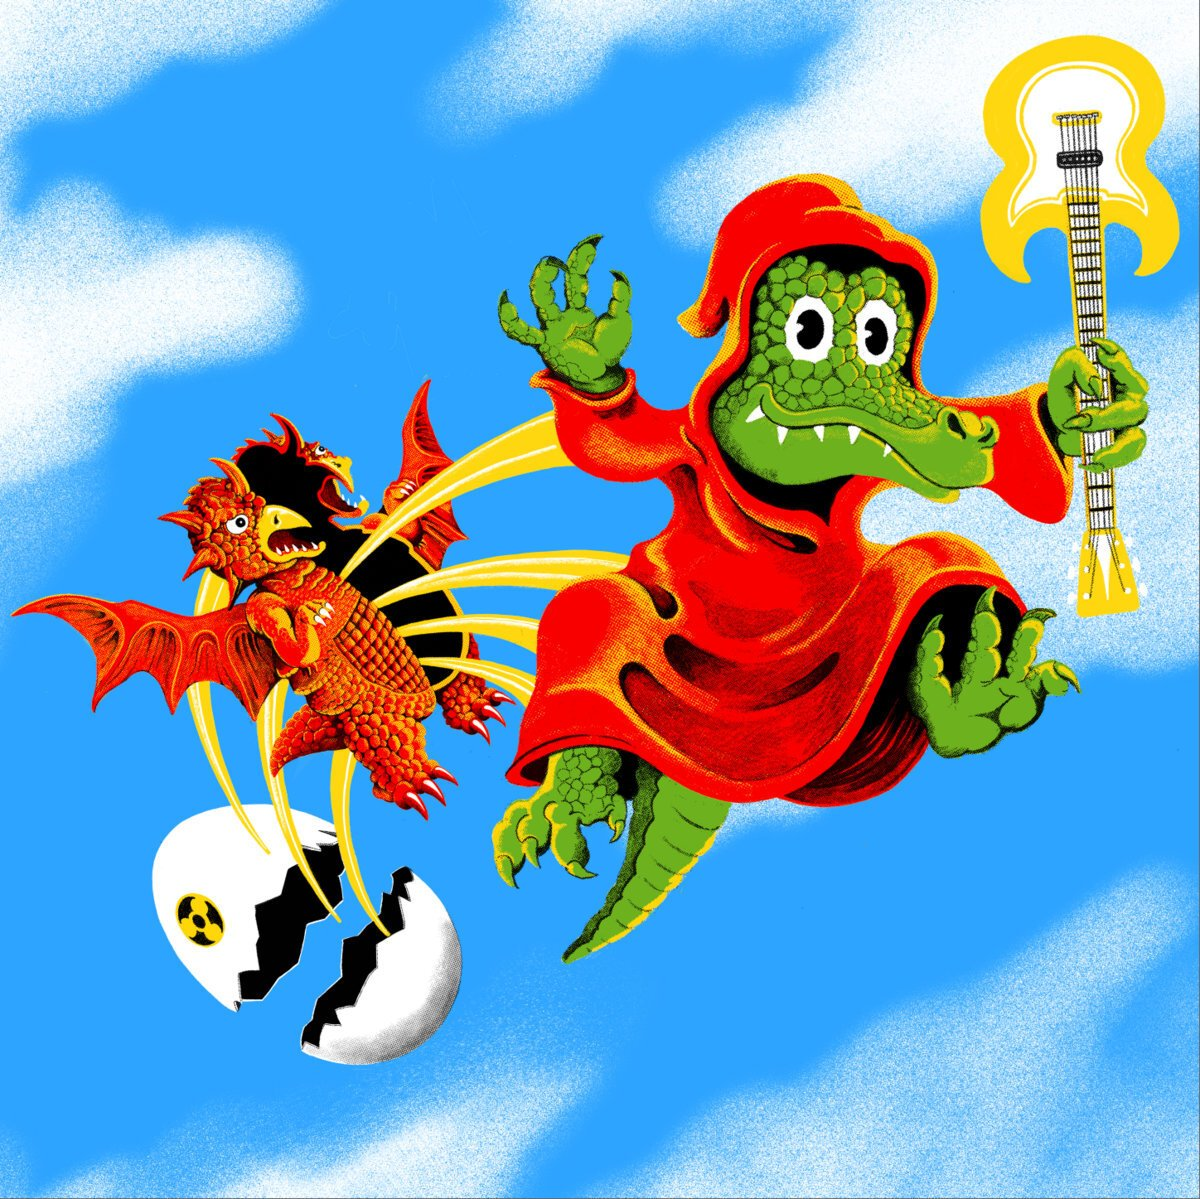
\includegraphics[width=0.8\linewidth]{cover-image.jpg}\\[2em]%
    \fi
    The Book\\%
    {\relscale{0.8} of Lyrics}%
}
\author{King Gizzard \& the Lizard Wizard}
\date{\textit{\relscale{0.8} Edition of \today}}

% Adjust head height for fancyhdr
\setlength{\headheight}{15pt}
\addtolength{\topmargin}{-3pt}

% This must be here, because defaults are set and renewcommand for section marks will work.
\pagestyle{fancy}

% Setup page headers/footers
\renewcommand{\chaptermark}[1]{\markboth{#1}{}}
\renewcommand{\sectionmark}[1]{\markright{\thesection\ #1}}

\fancypagestyle{fancy}{%
	\fancyhf{} % clear all fields
	\renewcommand{\headrulewidth}{1pt}
	\lhead{\nouppercase{\leftmark}}
	\rhead{\nouppercase{\textit{\rightmark}}}
	\lfoot{}
	\cfoot{\thepage / \pageref{LastPage}}
	\rfoot{}
}

\fancypagestyle{plain}{
	\fancyhf{} % clear all fields
	\renewcommand{\headrulewidth}{0pt}
	\cfoot{\thepage / \pageref{LastPage}}
}

\pagestyle{empty}

% Setup word underlining
\renewcommand{\ULdepth}{1.8pt}
\contourlength{0.8pt}

\renewcommand{\underline}[1]{%
    \uline{\phantom{#1}}%
    \llap{\contour{white}{#1}}%
}

% Center chapter titles and set spacing
\titleformat{\chapter}[display]
    {\normalfont\huge\bfseries\centering}
    {\centering\chaptertitlename\ \thechapter}{20pt}{\Huge}
\titlespacing*{\chapter}
    {0pt}{20pt}{40pt}

% Smart page break (when not enough space is left on the page)
\newcommand{\smartpagebreak}{%
	\Needspace{0.22\textheight}%
}

% Each section starts a new page (using smart page breaks)
\newcommand\sectionbreak{%
	\smartpagebreak%
}

% Fix TeX4ht issues where some commands are undefined
\ifdefined\theHchapter\else\newcommand\theHchapter{\Alph{chapter}}\fi

% Fix TeX4ht issue with non-escaped ampersand (&) characters in index entries
\newcommand{\textamp}{\ifdefined\HCode\string&\else\&\fi}
\newcommand{\textdol}{\ifdefined\HCode\string$\else\$\fi}
\newcommand{\textexcl}{\ifdefined\HCode\string!\else\string"!\fi}

%======================================================================

\begin{document}

% Define some shortcuts

% Helper function: add lowercase word to index.
% args: text
\newcommand{\lindex}[1]{%
  \lowercase{\def\temp{#1}}%
  \expandafter\index\expandafter{\temp}%
}

% Begin new album chapter.
% args: toc-title, title
\NewDocumentCommand{\album}{O{} m}{%
    \ifthenelse{\equal {#1}{}}{%
        \chapter{#2}%
    }{%
        \chapter[#1]{#2}%
    }%
    \nopagebreak%
}

% Add album subtitle.
% args: text
\NewDocumentCommand{\subtitle}{m}{%
    \vspace*{-3em}%
    \begin{centering}%
        \bfseries%
        #1%
    \end{centering}%
    \vspace*{2em}%
}

% Add album artwork.
% args: filename
\NewDocumentCommand{\artwork}{m}{%
    \vspace*{-2em}%
    \nopagebreak%
    \begin{center}%
		\iftex4ht%
			\includegraphics[width=0.5\linewidth]{artworks/#1}%
		\else%
			\includegraphics[width=0.5\linewidth]{artworks/#1}%
		\fi%
    \end{center}%
    \nopagebreak%
}

% Add album release date.
% args: year, month, day
\NewDocumentCommand{\released}{m m m}{%
    \vspace*{-1em}%
    \nopagebreak%
    \begin{center}%
        \textit{Released: \shortdate\formatdate{#3}{#2}{#1}}%
    \end{center}%
    \iftex4ht%
        \newpage%
    \fi%
    \nopagebreak%
}

% Add song title (with optional args for special entry in index/table of contents)
% args: index-title, toc-title, title
\NewDocumentCommand{\song}{O{} O{} m}{%
    \ifthenelse{\equal {#2}{}}{%
        \section[#3]{#3}%
    }{%
        \section[#2]{#3}%
    }%
    \ifthenelse{\equal {#1}{}}{%
        \index[songs]{#3}%
    }{%
        \index[songs]{#1}%
    }%
    \nopagebreak%
}

% Add credits for song lyrics ("Written by: xyz").
% args: text
\newcommand{\writtenby}[1]{%
    \nopagebreak%
    \textscale{.75}{[Written by: \textit{#1}]}%
	\newline\vspace{-.4\baselineskip}%
    \nopagebreak%
}

% Add note on vocals for song lyrics.
% args: text
\newcommand{\vocalsby}[1]{%
    \nopagebreak%
    \textscale{.875}{[\hspace{.12em}\textit{#1:}\hspace{.12em}]}%
	\newline\vspace{-.3\baselineskip}%
    \nopagebreak%
}

% Add note on vocals for song lyrics.
% args: text
\newcommand{\songsection}[1]{%
    \nopagebreak%
    \textscale{.875}{\textbf{#1}}%
	\newline\vspace{-.3\baselineskip}%
    \nopagebreak%
}

% Add a note to the song lyrics.
% args: text
\NewDocumentCommand{\note}{m}{%
    \nopagebreak%
    \emph{#1}\newline%
    \nopagebreak%
}

% Highlight a word/phrase and add it to the word index (lowercase.)
% args: text
\NewDocumentCommand{\word}{O{} m}{%
	\ifthenelse{\equal {#1}{}}{%
        \lindex{#2}%
    }{%
        \lindex{#1}%
    }%
	%\underline{#2}%
	\emph{#2}%
}

% Make title page
\maketitle

% Make frontmatter page
\begin{center}
{\relscale{0.8}%
\vspace*{\fill}%

This e-book collects all lyrics from the Australian band \emph{King Gizzard \& the Lizard Wizard}. \\[1em]
I started this project in June 2025 because I wanted to read Gizz lyrics on my e-book reader while listening to their music.
The included songs are grouped by album, and albums are added in chronological order (oldest first.)
There is also a song index at the end of the document that lists all songs in alphabetical order regardless of album,
and a word index that references selected words that are reoccuring throughout the lyrics. \\[1em]

Compiled by Jan Behrens (zykure). \\[1em]

This project is available on GitHub: \\
\href{https://github.com/zykure/KGLW-TheBook}{https://github.com/zykure/KGLW-TheBook} \\[2em]

All artwork and lyrics are copyright by \\
King Gizzard \& the Lizard Wizard and the respective authors. \\[2em]

\underline{Lyrics credits:} \\
Michael Cavanagh \\
Cook Craig \\
Lucas Harwood \\
Ambrose Kenny-Smith \\
Stu MacKenzie \\
Joey Walker \\[2em]

\underline{Artwork credits:} \\
Jason Galea \\[2em]

A big thanks to @michal-h21 for creating the TeX4ebook package: \\
\href{https://github.com/michal-h21/tex4ebook}{https://github.com/michal-h21/tex4ebook} \\[1em]

Shoutout to \\
\href{https://kglw.net}{\textit{kglw.net}}, \href{https://weirdoswarm.org}{\textit{weirdoswarm.org}}, \href{https://gizzheads.de}{\textit{gizzheads.de}} \\
and the Gizz global community! \\

\vfill%
}%
\end{center}


\pagebreak

% Print table of contents
\iftex4ht
\else
	\tableofcontents
	\thispagestyle{plain}
\fi

\pagestyle{fancy}

% Add lyrics
% (Albums)
\renewcommand{\chaptername}{Album}%
%
\album{12 Bar Bruise}

%----------------------------------------------------------------------

\song{Elbow}

\note{[Written by: Stu MacKenzie]}

You want\\
You got\\
You are such a big shot\\
You cunt you know me better\\
Than to bend my elbow back\\
Stab me in the back\\

EY EY EY EY EY EY EY EY\\

%----------------------------------------------------------------------

\song{Muckraker}

\note{[Written by: Stu MacKenzie]}

Clear the cobwebs off my brain\\
Ants have came\\
It smells like rain\\

Pissin' shit off porcelain\\
I'll rake the muck\\
It's just my luck\\

Oh no, oh no\\
Muckraker\\

%----------------------------------------------------------------------

\song{Nein}

\note{[Written by: Stu MacKenzie]}

Never, never, never, never,\\
Had much too much, I'm sick of it\\
My body's full of poison shit\\
Never, never, well, ha ha, ha, ha!\\

Shit, never again\\

One, two, three, four, five, six, seven, eight\\
Nein! Nein! Nein! Nein! Nein!\\

%----------------------------------------------------------------------

\song{12 Bar Bruise}

\note{[Written by: Stu MacKenzie]}

Better be slave\\
Make some money\\
So when it gets ruff\\
We can bruise some stuff\\

But look at my dick\\
I bet you it's limp\\
Should I quit drink\\
It makes me think that…\\

12 bar booze is\\
12 bar bruise\\

Gotta be strong\\
Make me live long\\
Better not wait\\
For a bottle's sake\\

All of my friends are\\
Looking up dresses\\
They have not seen\\
The bruise that I've seen\\
Broo-oo-oo-oo-uize\\

%----------------------------------------------------------------------

\song{Garage Liddiard}

\note{[Written by: Stu MacKenzie]}

My head\\
Oh my head\\
My head's all bleak\\
And it makes my love so rough\\

My knees\\
Oh my knees\\
My knees are weak\\
And it makes for walking tough\\

Oww! Oww! Oww! Ouch!\\

%----------------------------------------------------------------------

\song{Sam Cherry's Last Shot}

\note{[Written by: Stu MacKenzie]}

Early that morning, the wagon-master of the train\\
came into the post greatly excited,\\
and reported that the dead body of a man and horse\\
had been found in the road about six miles from the post.\\

A company of infantry was immediately ordered out,\\
and proceeding to the spot found the body of Sam Cherry,\\
pinned fast to the ground by the dead body of his horse.\\

The search was continued, and in the lateral canyon were found\\
the bodies of Sargent Love and the three privates loaded with bullets,\\
mutilated and disfigured, but giving every evidence\\
of having sold their lives as great men should.\\

Trails were examined and the whole story worked out.\\

The party traveled along the road nearly to the entrance\\
of the canyon of the Limpia, known as the "Wild Rose Pass,"\\
when suddenly about thirty mounted Indians\\
dashed from the bushes along the stream,\\
cutting it off from retreat towards the Fort,\\
and driving it up the lateral canyon.\\

Suspecting a trap, Sam Cherry suddenly turned,\\
dashed through the line of Indians,\\
regained the road, and ran for life, away from the Fort,\\
followed by a number of yelling savages.\\

He was evidently doing well, when his horse stumbled and fell,\\
breaking his neck, and pinning Sam's leg to the ground.\\
In an instant he was surrounded by the exultant Indians.\\

Raising himself slightly, Sam fired five shots at his enemies,\\
then turning the muzzle against his own temple, he escaped\\
the tortures of their vindictive rage by his "last shot."\\
The baffled and terrified Indians went away as fast\\
as their ponies could carry them,\\
not touching the body,\\
not even taking the arms.\\

Such is the way out in the west.\\
People die by extreme barbaric ways.\\
But we're taking their land,\\
and in return they take our viscera\\
and spread it across the desert plains.\\

%----------------------------------------------------------------------

\song{High Hopes Low}

\note{[Written by: Stu MacKenzie]}

Well I ain't dumb\\
But I ain't that smart\\
And I can't spell\\
But I can sound it out\\

Gotta keep your high hopes low\\

%----------------------------------------------------------------------

\song{Cut Throat Boogie}

\note{[Written by: Stu MacKenzie \& Ambrose Kenny-Smith]}

As a child I felt inclined\\
To fold my ears in twine\\
Never once was I confined\\
I picked and choosed about my ride\\
So buckle me in before we set sail ahead\\
For it smells like cabbage\\
Got way too stale like death\\

Oh you're white as a ghost\\
I never felt so pale\\
As the blood dripped across the floor\\

So put it buried in your chest\\
With the rest of your drunken regrets\\
Inches from your jugular\\
As the room fills in front of ya\\
It took them long enough\\
For them to stop and suggest\\
Hey we better get him some help\\
We better get him out of here\\

How did I manage to cope as the blood soaked\\
Through my clothes and to the floor\\
From outside to the bathroom door\\
I was inches from my life\\
Yeah that's what keeps me up at night\\

Oh how did I survive / you shoulda died\\
How did I manage to cope / being alive\\
After all it was just a / innocent play fight\\
I hope they don't stop to sympathise\\

Stitch up the past to cure their whoremented heart\\

Tormented dreams it's all left in between…\\

%----------------------------------------------------------------------

\song{Bloody Ripper}

\note{[Written by: Stu MacKenzie]}

Push me down I will not crack\\
You're just a monkey with your claws in my back\\
I said it, and you heard\\
That murky bottle's cuttin' me some slack\\

But it's like all I wanna do\\
Sink my teeth in you\\
You already told me to\\
You said it's alright\\

%----------------------------------------------------------------------

\song{Uh Oh, I Called Mum}

\note{[Written by: Stu MacKenzie]}

Uh oh, uh oh\\
Uh oh, uh oh\\
Uh oh, uh oh\\
Uh oh, uh oh I called Mum!\\

I bought a funny glob\\
I put it in my gob\\
I had anxiety\\
I couldn't help myself\\
But call Mum\\

%----------------------------------------------------------------------

\song{Sea of Trees}

\note{[Written by: Stu MacKenzie]}

Oh hell I'm feeling underwater\\
My head is sinking like a stone\\

And hell I'm feeling kinda sick / like a prick\\
I don't know what's the use in it\\

And when you're feeling suicidal\\
Sometimes you've just got to unfold\\

%----------------------------------------------------------------------

\song{Footy Footy}

\note{[Written by: Stu MacKenzie \& Joey Walker]}

Footy footy\\
All I wanna do is\\
Footy footy\\
All I wanna kick is\\
Footy footy\\
Catch the ball, kick play on!\\
Crumb the ruck, run, handball!\\
Footy footy\\
Footy! Footy! footy!\\

Ang Cristou, Che Cockatoo-Collins,\\
Phillip Matera, Gavin Wanganeen,\\
Gary Moorcroft, Aussie Jones,\\
Bruce Doull The Flying Doormat,\\
Spider Everett, Spider Burton,\\
Craig Bradley,\\
The 1995 Carlton football team\\

Footy footy\\
Footy footy\\
Footy footy\\
Footy footy\\

Diesel Williams, Dale Kickett,\\
Sticks Kernahan, Darren Jarman,\\
Chad Rintoul, Ashley Sampi,\\
Mick Martin, Clint Bizzell,\\
The Brisbane Bears,\\
Aaron Hamill, everyone…\\

I'm gonna go down to Waverley Park\\
I'm gonna sit on the wing\\
I'm gonna eat a pie\\
I'm gonna buy a footy record for a dollar fifty\\
I'm gonna have a full strength beer ya girl\\
I'm gonna take a specky\\
I'm gonna kick a banana\\
I'm gonna eat a banana\\
I am gonna love every second of it\\
I hate what this game has become.\\
								% DONE
\album{Eyes Like The Sky}

\artwork{eyes-like-the-sky.jpg}
\released{2013}{02}{22}
\label{album:eyes-like-the-sky}

%----------------------------------------------------------------------

\song{Eyes Like The Sky}

\writtenby{Mackenzie/Smith}

\vocalsby{[All songs narrated by Broderick Smith]}

The bad, white men call him the \word{devil}. The \word{Yavapai} call him ``Eyes Like the \word{Sky}.'' \\

This story takes place in the hinterlands of the newly formed United States and territories in the years before and after the great conflagration called the Civil War. Men roam and fight each other simply to stay breathing. Muskets give way to repeating rifles, cannons give way to Gatling guns. War nurtures weapons, weapons clear the land. \\

In the \word[desert]{deserts} of the southwest, old hatreds grow into new ones. Old beliefs are shattered by gunfire and charging horses. Into this cauldron of fire rides a young man who becomes a shadowed legend. His name even takes on the mantle of the \word{boogieman} in some homes. \\

Among the first Americans, his name is exalted from wickiups to longhouses from teepees to cliff dwellings. Among the men of the badlands, he is feared for his silent walk and swift, economical dispatching of his enemies. \\

%----------------------------------------------------------------------

\song{Year Of Our Lord}

\writtenby{Mackenzie/Smith}

\songsection{Chapter 1}

They'd been watching the farmhouse for a while, maybe all day. There were two of them, both young and fit and \word{desert}-hardened. They were lords of where they lived and they had no foreign teachings from white men or Mexicans. \\

Except for one thing. They hated the Mexicans more than the white men because of their cruelty, and they'd learned cruelty from the Mexicans very well in return. \\

The smoke from the mud house curled up into the \word{sky} like an albino \word{snake}. The two young men watched and counted the white men down in the farmyard. A tall man and two shorter ones, maybe his sons. A woman would occasionally come out from the shack, get water from the well in the front yard and carry it back inside. A small child would be with her. \\

The men watching on the rim had no calendars, so they didn't know the date. 12th of June, year of our Lord, 1854. \\

But one thing they did know: About an hour away were the rest of their party. Eight men, all armed, running smoothly and trackless over the rocks. One of the watchers moved away to tell the main party of what they had seen. \\

The raid was about to start. \\

%----------------------------------------------------------------------

\song{The Raid}

\writtenby{Mackenzie/Smith}

They were not after the money, they were not after alcohol. They were after guns and young children to raise as their own. War had made it necessary to take child captives. The rest would be slaughtered. \\

And that is how \word{Miguel O'Brien} became a \word{Yavapai}-Apache warrior.
He was five years old. \\

%----------------------------------------------------------------------

\song{Drum Run}

\writtenby{Mackenzie/Smith}

\songsection{Chapter 2}

\word{Miguel O'Brien} ran with the Apaches. He ran and ran, and as his legs grew he glided over the \word{desert} earth. He learned how to hide and to hunt. He learned to leave no tracks and he learned to live on what he could keep down. And his name was now ``Eyes Like The \word{Sky}''. \\

His blue eyes showed his father's race. He never wore the white painted face of the slave. He was valued for his stamina and distant vision. By the time he was 15, he had already killed Mexican troopers and feared no man. \\

%----------------------------------------------------------------------

\song{Evil Man}

\writtenby{Mackenzie/Smith}

It is 1864 now, and the American's war has not come to the \word{desert} lands. They fight among themselves way off to the north. The \word{Yavapai}-Apache are still lords of all they survey. \\

Then one morning the Americans did come, led by a man holding a leather book with a cross stamped in the leather. An evil man who did terrible things to people, in the name of a \word{God} that looked upon the man himself with revulsion. \\

\word[Miguel O'Brien]{Miguel} ran from his wickiup, half asleep when they attacked. A rifle butt sent him unconscious. When he came to, he was trussed-up, on his back, on the ground, looking up at the Americans. He had not been killed because they had noticed his blue eyes and knew he was one of them. \\

So at the age of 16, Miguel was back among his father's people. But once more a family he loved had been killed. This time by Americans. \\

%----------------------------------------------------------------------

\song{Fort Whipple}

\writtenby{Mackenzie/Smith}

\songsection{Chapter 3}

The Americans took the trussed-up boy to a place called \word{Fort Whipple}, a fly-blown group of tents surrounded by a stone and timber stockade. \\

An American called Willis was the boss there and he glared at the man of \word{God} as he entered with his captives. He noticed the boy when he was brought in with a few \word{Yavapai} girls and he looked into the colour of his eyes. \\

``What do you make of him?'' he asked the God man. \\
``He may be the young \word[Miguel O'Brien]{O'Brien} boy who was lost here years ago, or he could be from the Jepson party that never made it to New Mexico,'' said the God man back. \\

They named the boy Jepson O'Brien but the natives and frontiersmen called him ``Blue'', because of his eyes but also because of the baleful, almost sad expression he carried on his face. The expression of someone who kills with compassion but not mercy. \\

Although he was still a boy, the men mostly kept away from him. All except for one, a trapper who understood his skills, and in return, fed him and taught him the white man's way. In a short while, he could speak, read, and write their language, and he also added the calm, fast dignity of the gunman to his arsenal. \\

He was so fast that men treated him with care. But he was slow to anger and when angry, swift and final in his reply. In the Arizona \word{desert} in the 1860's, he had every skill that you needed to survive. And he was just 17. \\

%----------------------------------------------------------------------

\song{The God Man's Goat Lust}

\writtenby{Mackenzie/Smith}

\songsection{Chapter 4}

The \word{God} man with the \word{Bible} was in the back room of the chapel at \word{Fort Whipple}. The God man was deeply engrossed in satisfying his goat-lust with a \word{Yavapai} girl. She never said a damn thing but just leaned over an altar while he defiled her. He held a pistol to her head as he grunted away and when it was finished he shoved her towards the outside door. \\

But the God-man never got to fixing his long-johns or his black trousers. The young man named ``Blue'' strode softly up behind him and drove a long-bladed \word{knife} into his neck. Blood spurted into the chalice on the altar, but not the blood of the Christ. Just the blood of the God man. \\

With a cough he \word[die]{died}. And a bubbled gurgle. \\

The young man named Blue took the Yavapai girl, money, guns and food, and two strong horses and rode into the \word{desert}, away from Fort Whipple. The God man's body was found but he was not missed. \\

%----------------------------------------------------------------------

\song{The Killing Ground}

\writtenby{Mackenzie/Smith}

\songsection{Chapter 5}

For days they traveled, the young man and the \word{Yavapai} girl. She told him her name and they spoke in the language. They rode the horses until they gave out, then their throats were slit and meat was taken to eat later. No fires were lit, and they ate berries and raw jackrabbit as well to keep going. After a week they relaxed more as they entered Apacheria. \\

They saw dust way off like dust devils, but they knew it was horses. They could hear shots and no more. When all was quiet a day later, they moved silently towards the killing ground. \\

The buzzards told them the story before they got there. Dead white people, a lot of them, maybe a half dozen and burnt wagons and arrows. But not from one tribe. Some of the arrows were different and shod hoofmarks and moccasin tracks that were shaped like a white man's way of walking. Some white men had done this, loosely disguised as Apache. \\

They took what they could use and walked on. The purple mountains and red ochre earth swallowed them up and the young man smelt his own blood as they ran. And it was a good smell. \\

The smell of being alive. \\

%----------------------------------------------------------------------

\song{Dust In the Wind}

\writtenby{Mackenzie/Smith}

Suddenly the girl pitched sideways and a split second later the young man heard the distant shot. He dived for some rocks and watched as more bullets hit the girl. The young man looked to her body, and as she \word[die]{died} he worked out where the shots were coming from. \\

And he knew that \word{death} was going to walk among the shooters. \\

\songsection{Chapter 6}

There is one thing a white man should never do, and that is move towards an Apache because you will never get there. How do you catch dust in the wind? The young man saw the way they were coming by the movement of insects and birds and he knew where to go. Like the \word{snake} he slithered into a dry arroyo and worked behind the shots in an arc. \\

After a while he saw them. Three men, three white men clad in skins and they walked confidently towards the girl. The young man knew somewhere behind them another one held the horses, making four all together. \\

He moved towards that man. The killers could wait. Let them enjoy the hunt before they went under. He found the one by the horses. He was young too and \word[die]{died} quietly with a surprised indignant look on his face. The young man tied the horses to a tree. They'd come in handy later. Four horses and equipment. \\

At the girl's body, two men knelt beside her while another stood guard. The guard suddenly cried out as his head exploded in a bubble of pink spray and he fell forward. The other two went to ground and nervously called out to each other. \\

``Do you see the bastard?'' -- ``No, he must be close.'' \\

But he wasn't. A Sharp's sporting rifle will reach a long way in the right hands. The young man took careful aim and the smaller of the two men felt his right leg blasted away. The bigger, heavier man sank as far into the ground as he could make himself go. And still he could not see where the young man was. \\

%----------------------------------------------------------------------

\song[Guns \textamp{} Horses]{Guns \& Horses}

\writtenby{Mackenzie/Smith}

The young man by now was astride a horse and making for a \word{Yavapai} stronghold, half a day's ride away. He had more guns and horses than he needed, and he knew where two white men were sitting in the \word{desert} with no water and no horses. White men dressed as Yavapai Apaches. \\

The white men would be calling for their \word[mother]{mothers} and their \word{God} by evening. The young man would be drunk on tiswin and full of deer meat. And satisfied by their agony. \\
                          % DONE
\album{Float Along -- Fill Your Lungs}
\artwork{float-along-fill-your-lungs.jpg}
\released{2013}{08}{27}
\label{album:float-along-fill-your-lungs}

%----------------------------------------------------------------------

\song{Head On/Pill}

\note{[Written By: Mackenzie]}

Just yesterday I sat across from my legs. \\
They weren't connected to me. \\
I couldn't see because my eyes weren't in me. \\
Hold me up straight while I screw my head on. \\

Head on. \\

Just yesterday I held the cup to my lips. \\
Pouring it deep in my throat. \\
Filling up me like a black enemy. \\
Hold me up straight while I screw my head on. \\

Head on… \\

I ate the wrong pill… \\

%----------------------------------------------------------------------

\song{I'm Not a Man Unless I Have a Woman}

\note{[Written By: Mackenzie]}

Well, I'm not a man unless I have a woman. \\
Well, I'm not a man unless I have a woman. \\

She's a hundred pounds of gold. \\
(Yes I am.) \\
She's a hundred pounds of gold. \\
(He's a hundred pounds of gold.) \\
I got mine so I don't mind - no. \\

I'm not a woman unless I have a man. \\
I'm not a woman unless I have a man. \\

I ain't gonna break your heart. \\
(Yeah, I know you won't.) \\
Because I'm done breaking hearts. \\

%----------------------------------------------------------------------

\song{God Is Calling Me Back Home}

\note{[Written By: Mackenzie]}

Meet me at the house on the top of the hill. \\
I've got two important people that I'm ready to kill. \\
I'll just flunk or fail so give me something better to do. \\

Santa's on the roof with his presents and sack. \\
He's got one hand with a blade and the other's an axe. \\
I'll just flunk or fail so give me something better to do. \\

Then I hear \word{God} call. \\
And all my hate is gone. \\
I hear him calling me back home. \\

Oh I heard God call. \\
And now my hate is gone. \\
I heard Him calling me back home. \\

God is calling me back home… \\

%----------------------------------------------------------------------

\song{30 Past 7}

\note{[Written By: Mackenzie]}

At 30 past 7 you know I could be better. \\
At 30 past 2 I'll get along with you. \\
I'm grumpy in the morning. \\
You know that when I'm yawning it's true. \\

That I'll be snappy towards you. \\
That I'll bite pieces out of you. \\

%----------------------------------------------------------------------

\song{Let Me Mend the Past}

\note{[Written By: Mackenzie/Kenny-Smith]}

Let me mend the past. \\
Let me see behind your mask. \\
You finally go around. \\
She stares at the ground. \\
And acts if you're not there. \\

Locks on the door. \\
Surveillance when you enter in \\
The hall such a pointless cause. \\
Her cups on my wall. \\
It's hard to be ignored. \\

Let me mend the past. \\
And make ends meet at last. \\
Before they bleed. \\
Don't wanna come across too weak. \\

Let me mend the past. \\
Let me mend the past. \\
This will be the last time I ask. \\
Let me mend the past. \\

%----------------------------------------------------------------------

\song{Mystery Jack}

\note{[Written By: Mackenzie]}

I am my mother's son. \\
And I'll keep doin' 'till the done gets done. \\
I wouldn't steal for free. \\
And I won't see you next to me. \\

'Cos I, oh I. \\
I, oh I hope I don't wake up. \\

'Cos I'm a lonely soul. \\
And I've got no friends on this road. \\
And I'm a mystery Jack. \\
The lines on my hands tell me I'm on track to die. \\

Oh, die. \\
'Cos I, oh I hope I don't wake up. \\

%----------------------------------------------------------------------

\song{Pop In My Step}

\note{[Written By: Craig]}

Gonna shake the world, shake the world off my back. \\
I'm gonna hold my head high with the sun on my track. \\
Today I've got no troubles in sight. \\

Gonna put some pop in my step when I walk. \\
I'm gonna show my mood off when I walk and I talk. \\
Today I've got no troubles in sight. \\
Gonna turn around make everything that was wrong into right. \\

Gonna look past things that I know I'll regret. \\
Cause life's a little too short for those worries, you can bet on me. \\
Today I've got no troubles in sight. \\
Gonna turn around, make everything that was wrong into… \\
Right, right. \\

When I wake up late in the morning you'll know. \\
It takes a few more hours before I'll know. \\
Today I've got no troubles in sight. \\
Gonna turn around make everything that was wrong into… \\
Right, right, right, right. \\

%----------------------------------------------------------------------

\song{Float Along -- Fill Your Lungs}

\note{[Written By: Mackenzie]}

I saw you in the carpet shades. \\
Then I felt you like a baby's face. \\
Just float along and fill your lungs. \\
Float along and breathe a deep breath. \\

I saw you in the paper folds. \\
And I saw you in my coffee mug. \\
Just float along and fill your lungs. \\
Float along and breathe a deep breath. \\

Just float along and fill your lungs. \\
Just float along and fill your lungs. \\
Just float along and breathe a deep breath. \\
Just float along and fill your lungs. \\
								% DONE
\album{Oddments}

\artwork{oddments.jpg}
\released{2014}{03}{07}
\label{album:oddments}

%----------------------------------------------------------------------

\song{Alluda Majaka}

\writtenby{Mackenzie}

\note{(Instrumental)}

%----------------------------------------------------------------------

\song{Stressin'}

\writtenby{Mackenzie/Walker}

\vocalsby{Stu Mackenzie}

I'm stressin' \\
About what I've been missin'. \\
And I'm feeling stressin' is an instinct. \\
Stress colours all of my dreams orange. \\
I'm dreaming stressin' is an instinct. \\
Now I'm biting down on my jaw. \\
Oh, now it's making all my teeth sore. \\

Seein' trouble. \\
One thing to another. \\
I'm feeling stressin' is an instinct. \\
My partner is a clever lover. \\
She told me stressin' is an instinct. \\
Now I'm biting down on my jaw. \\
Oh, now it's making all my teeth sore. \\

I'm stressin' \\
About what I've been missin'. \\
And I'm feeling stressin' is an instinct. \\
Stress colours all of my dreams orange. \\
I'm dreaming stressin' is an instinct. \\

%----------------------------------------------------------------------

\song{Vegemite}

\writtenby{Mackenzie}

\vocalsby{Stu Mackenzie}

I love, I love my \word{Vegemite}, \\
It's strong as Hell and black as night. \\
I keep my \word{love} all screwed up tight \\
And spread it thick whenever \\
I like, I like… \\

Vegemite. \\
I like. \\
Vegemite. \\
I like, I like… \\

And when everyone's getting grumpy 'cos it's early, \\
I'll have breakfast with my girlfriend. \\
And we'll have toast with avocado \\
And tomato \\
And Vegemite. \\

'Cos I love, I love my \word{Vegemite}. \\
It's strong as Hell and black as night. \\
I keep my love all screwed up tight \\
And spread it thick whenever \\
I like, I like… \\

Vegemite. \\
I like. \\
Vegemite. \\
I like, I like… \\

%----------------------------------------------------------------------

\song{It's Got Old}

\writtenby{Mackenzie}

\vocalsby{Stu Mackenzie}

I'm always saying I'm sorry \\
And you're always saying you're broke. \\
I'll keep my hands on the steering \word{wheel} \\
If you keep your eyes on the road. \\
But it's not like you anyway \\
To hide your sad face away. \\
It ain't gonna stay the same, \\
'Cos it's got old. \\

You'll always run me in circles, \\
Chasing me round like a mouse. \\
I'll keep on watching this movie \\
If it means I can stay at your house. \\
But it's not like you anyway \\
To hide your sad face away. \\
It ain't gonna stay the same, \\
'Cos it's got old… \\

%----------------------------------------------------------------------

\song{Work This Time}

\writtenby{Walker/Mackenzie}

\vocalsby{Joey Walker}

I knock, hello, but I see \\
That you've got hypothermia. \\
So I place a block to stop the rot \\
And hope that I can warm you up. \\

Do I have to shake you, babe, \\
Until you're blind? \\
Cause every light bulb's blown \\
And I'm feeling so inclined. \\

Can never lay my whole head down… \\
I know I'm lazy, \\
But baby I will work this time. \\

It's kind of funny that I live \\
The poetry I can not write. \\
But you, my beauty, shall be fixed \\
Forever loosely in my heart. \\

Do I have to shake you, babe, \\
Until you're blind? \\
Cause every light bulb's blown \\
And I'm feeling so inclined. \\

Can never lay my whole head down… \\
I know I'm lazy, \\
But baby I will work this time. \\

%----------------------------------------------------------------------

\song{ABABCD}

\writtenby{Walker}

\vocalsby{Stu Mackenzie \& Joey Walker}

Ababcd. \\
Will show you how it feels \\
To be stuck outside your sanity \\
And wrapped around infinity. \\
I want to leave but I can't conceive that \\
I'll snap back to reality. \\

%----------------------------------------------------------------------

\song{Sleepwalker}

\writtenby{Mackenzie}

\vocalsby{Stu Mackenzie}

Ooh, ooh, hee, hee, hee. \\
Ooh, ooh, hee, hee, hee. \\
Ooh, ooh, hee, hee, hee. \\
Well I want to, I want to, I want to. \\
I want to walk in your shoes. \\
Oh No! \\

Ooh, ooh, hee, hee, hee. Sleepwalker. \\
Ooh, ooh, hee, hee, hee. Sleepwalker. \\
Ooh, ooh, hee, hee, hee. \\
Well I want to, I want to, I want to \\
I want to sleepwalk with you. \\
Oh No! \\

I caught you sleeping on the wrong side of the bed. \\
So I got up and switched my side. \\
Your voice gets hoarse when you get too cold. \\
I'll warm you up. Wo-oh! Warm you up. \\
Ooh, ooh, hee, hee, hee. Sleepwalker. \\
Ooh, ooh, hee, hee, hee. \\
(Sleep. Sleep. Sleepwalker.) \\

If you're thinking then you're thinking too hard. \\
So squish your brain and numb your pain. \\

Ooh, ooh, hee, hee, hee. Sleepwalker. \\
Ooh, ooh, hee, hee, hee. Sleepwalker. \\
Ooh, ooh, hee, hee, hee. \\
Well I want to, I want to, I want to \\
I want to sleepwalk with you. \\
Oh No! \\
Ooh, ooh, hee, hee, hee. \\

%----------------------------------------------------------------------

\song{Hot Wax}

\writtenby{Mackenzie/Kenny-Smith}

\vocalsby{Stu Mackenzie}

Hot wax comin' under the door. \\
Hot wax comin' under the floor. \\
Hot wax creepin' under the hill. \\
Hot wax creepin' under the sill. \\

Hot wax, c'mon get around. \\
Everybody's learning how. \\
Come on a safari with me. \\

Hot wax. Hot wax… \\

\vocalsby{Ambrose Kenny-Smith}

Hot wax slippin' under the seat. \\
Hot wax drippin' under the feet. \\
Hot wax leakin' under the sink. \\
Hot wax leakin' under the drink. \\

\vocalsby{Stu Mackenzie}

Hot wax comin' under the lord. \\
Hot wax comin' under the door. \\
Hot wax comin' into the brain. \\
Hot wax comin' into the maze. \\

Hot wax, c'mon get around. \\
Everybody's learning how. \\
Come on a safari with me. \\

Hot wax. Hot wax… \\

Hot wax, c'mon get around. \\
Everybody's learning how. \\
Come on a safari with me. \\

Hot wax. Hot wax… \\

\vocalsby{Ambrose Kenny-Smith}

Hot wax slippin' under the seat. \\
Hot wax drippin' under the feet. \\
Hot wax leakin' under the sink. \\
Hot wax leakin' under the drink. \\

Hot wax risin' from beneath. \\
Hot wax risin' from the leaves. \\
Hot wax runnin' under my bed. \\
Hot wax runnin' up my leg . \\

Hot wax. Hot wax… \\

%----------------------------------------------------------------------

\song{Crying}

\writtenby{Craig}

\vocalsby{Cook Craig}

Came in my window crying. \\
Said that she's sick of all his lying about me. \\
I said I ain't got time for her. \\
I'm gonna close the door when I go walking \\
Out! Out! Out! Out! \\

Came to me Monday Morning. \\
Interrupted me in my mid-morning yawning. \\
He said the same thing that she said. \\
Well I just turned to him and said that she ain't \\
Mine! Mine! Mine! Mine! \\

Baby, you always acted \\
Like, baby, you never cared. \\
With the way you act girl, \\
You're bound to make your guy \\
Cry! Cry! Cry! Cry! \\

Well I ain't gonna be the one \\
To watch you fall down the stairs. \\
With the way you act girl, \\
You're bound to make your guy \\
Cry! Cry! Cry! Cry! \\

%----------------------------------------------------------------------

\song{Pipe-Dream}

\writtenby{Craig}

\note{(Instrumental)}

%----------------------------------------------------------------------

\song{Homeless Man In Adidas}

\writtenby{Mackenzie}

\vocalsby{Stu Mackenzie}

I'm not lonely… \\
The city keeps me company… \\

Sit on the roof. \\
Watch the cars travel past. \\
Ain't no way of getting lonely. \\
And I'll sit real still and watch everyone go fast. \\
With only me. \\

Lay on the bay. \\
Watch it all float away. \\
Ain't no way of getting lonely. \\
Watch all the people and the bikes come my way. \\
With only me. \\

I'm not lonely… \\

%----------------------------------------------------------------------

\song{Oddments}

\writtenby{Mackenzie}

\vocalsby{Stu Mackenzie}

Oddments. \\
There is nothing to care. \\
'Cos it's all that I will ever do. \\
Odd-Ments! \\

O-D-D-M-E-N-T-S! \\
                                   % DONE
\album{I'm In Your Mind Fuzz}

\artwork{im-in-your-mind-fuzz.jpg}
\released{2014}{10}{31}
\label{album:im-in-your-mind-fuzz}

%----------------------------------------------------------------------

\song{I'm In Your Mind}

\writtenby{Mackenzie}

Everybody's lazy when they're tired. \\
Because everybody's sucking on fluoride. \\
And everybody's filing into line. \\
Because everybody's sucking on fluoride. \\. \\

When I'm in your mind. \\
Then I'm in your mind. \\

While everybody wants to suck you dry. \\
And dig a little deeper in your mind -- c'mon, deeper. \\
Everybody's lazy because they're fried. \\
Because everybody's sucking on fluoride . \\

%----------------------------------------------------------------------

\song{I'm Not In Your Mind}

\writtenby{Mackenzie}

\note{(Instrumental)}

%----------------------------------------------------------------------

\song{Cellophane}

\writtenby{Mackenzie}

Do-do-do-do. \\

You can watch your movies in 3D. \\
It's so strange. \\

With cellophane, cellophane. \\
Cellophane, cellophane. \\
Cellophane, cellophane. \\
Cellophane, oh. \\
Do-do-do-do. \\

You can color everything you see. \\
It's so strange. \\

With cellophane, cellophane. \\
Cellophane, cellophane. \\
Cellophane, cellophane. \\
Cellophane, oh. \\
Do-do-do-do. \\

You can watch your movies in 3D. \\
It's so strange. \\

With cellophane, cellophane. \\
Cellophane, cellophane. \\
Cellophane, cellophane. \\
Cellophane, oh. \\
Do-do-do-do. \\

%----------------------------------------------------------------------

\song{I'm In Your Mind Fuzz}

\writtenby{Mackenzie}

When I'm in your mind. \\
Then I'm in your mind. \\
When I'm in your mind fuzz. \\
Then I'm in your mind . \\

%----------------------------------------------------------------------

\song{Empty}

\writtenby{Mackenzie}

Empty. \\
Life is nothing like it used to be. \\
People used to be so nice to me. \\
Feeling so empty. \\
Empty. \\
There is nothing deep inside of me. \\
Love is nothing like it used to be. \\
Feeling so empty. \\

Life is death. \\
It's because I shot it through its head. \\
I'm wandering around so lazily. \\
And feeling so empty. \\
And now I know. \\
It's because I never set it stone. \\
And I'm wandering around so lazily. \\
Feeling so empty. \\

But I don't feel empty when I'm with you. \\
I feel like you level me too. \\
Who? Empty. \\

What I got myself into. \\

%----------------------------------------------------------------------

\song{Hot Water}

\writtenby{Mackenzie/Walker}

Eat up. \\
Vomit. \\
Date line. \\
Repay. \\
System failure. \\
Wish for old way. \\
Straighten. \\
Bend it. \\
Decline. \\
Spend it. \\
Believe sceptic. \\
Everybody's standing in. \\

Hot water. \\

Sheet of paper. \\
Mountain raper. \\
Moment silence. \\
I am spineless. \\
Echoes ending. \\
Whispers trending. \\
Heat is coming. \\
Everybody's stranded in. \\

%----------------------------------------------------------------------

\song{Am I In Heaven?}

\writtenby{Mackenzie}

I've got ideas in my brain about the end of the world that I won't even say. \\
When all the bricks that built our brains will be turned into sand by the eternal wave. \\
If we save her we'll live on a star because mother nature made everybody else so far. \\

Am I in heaven? \\

Well everybody that I knew has jumped right in and taken over you. \\
And I swear even the ocean's changed its hue. \\
The lesson rings again. \\
Repeats within my brain. \\
Let's all put her to the test. \\
C'mon suck our mother's breast. \\

And everybody that I knew has taken bits and pieces out of you. \\
And I swear even the sky has changed its blue. \\
The lesson rings again repeats within my brain. \\
Let's all put her to the test. \\
C'mon suck our mother's breast. \\

%----------------------------------------------------------------------

\song{Slow Jam 1}

\writtenby{Mackenzie}

I need to slow my mind down low. \\

When it feels like coming on. \\
Boy it makes it hard to talk for me. \\

%----------------------------------------------------------------------

\song{Satan Speeds Up}

\writtenby{Mackenzie}

You brought us to your gift of generosity. \\
And all our silly games wreak havoc on your soils. \\
When I stop to think of all that. \\

Every life is like a song that takes forever to be sung. \\
When all our silly games wreak havoc on our spoils. \\
When I stop to think of all that we've done. \\
\word[satan]{Satan's} at the door. \\

Every second, every minute, every hour, every day. \\
He's watching you \\
And passing judgement to everybody you hold dear. \\
When I stop to think of all that we've done. \\
Satan's at the door. \\
Who's he looking for? \\

%----------------------------------------------------------------------

\song{Her and I (Slow Jam 2)}

\writtenby{Mackenzie}

It wouldn't hurt to give you more of my love. \\
The sun shone through into a wave of thought. \\
It said the one I'll wed has got a thinking head on her. \\
Her will will shine from up above on us. \\

Because every day I build on precious her and I. \\
It wouldn't hurt to put in some work on this angel. \\
I'll fill her heart with a lot of love. \\
So the sun can shine a little brighter. \\

On her and I. \\
						% DONE
\album{Quarters!}

\artwork{quarters.jpg}
\released{2015}{05}{01}
\label{album:quarters}

%----------------------------------------------------------------------

\song{The River}

\writtenby{Mackenzie}

\vocalsby{Stu Mackenzie}

Once you're in the zone \\
The \word{river} flows down like a full stone. \\
Water is your bed, \\
The ripples cushion your head. \\

I can't believe it. \\
It is frozen. \\
It's not the first time. \\
I had noticed. \\
She will deliver. \\
I am floating. \\
Trust in the river. \\
I had floated down, floated down. \\
Floated down, floated down. \\

\vocalsby{Stu Mackenzie \& Ambrose Kenny-Smith}

Floated down, down down, down down, down… (The river) \\
Down, down down, down down, down… (The river) \\

\vocalsby{Stu Mackenzie}

Once you're where I led \\
It will be clear what I had said. \\
Float without a home. \\
The river flows like another long road. \\

I can't believe it. \\
It is frozen. \\
It's not the first time. \\
I had noticed. \\
She will deliver. \\
I am floating. \\
Trust in the river. \\
I had floated down, floated down. \\
Floated down, floated down. \\

\vocalsby{Stu Mackenzie \& Ambrose Kenny-Smith}

Floated down, down down, down down, down… (The river) \\
Down, down down, down down, down… (The river) \\

Frozen over home. \\
The fading light shines on the white stone. \\
Melt your little zone. \\
And sink into the waterfall flow. \\

I can't believe it. \\
It is frozen. \\
It's not the first time. \\
I had noticed. \\
She will deliver. \\
I am floating. \\
Trust in the river. \\
I had floated down, floated down. \\
Floated down, floated down. \\

\vocalsby{Stu Mackenzie \& Ambrose Kenny-Smith}

Floated down, down down, down down, down… (The river) \\
Down, down down, down down, down… (The river) \\

%----------------------------------------------------------------------

\song{Infinite Rise}

\writtenby{Mackenzie}

Set straight. \\
Vibrate. \\
Need a hug. \\
Coffee mug. \\
Minor flop. \\
Don't stop. \\

What's more? \\
What's it for right now? \\

Days drop. \\
Hearts stop. \\
Days we've traveled. \\
And hearts unraveled. \\
Heart attack. \\
Hit me back. \\
Pigsty. \\
Don't cry. \\

Cat's eyes. \\
Capsize. \\
Making time. \\
Lifeline. \\
Limelight. \\
No right. \\

What's more? \\
What's it for right now? \\

Nice light. \\
Sunrise. \\
Bound together. \\
Like boys in leather. \\
Raisin bread. \\
Wreck the head. \\
Crack pipe. \\
Red light. \\

\word{Satan}. \\
Is hatin'. \\
Days old. \\
Bread mould. \\
\word{Jesus}. \\
Kills us. \\
Exalt. \\
My fault. \\

Daylight. \\
Insight. \\
Free roam. \\
Go home. \\
Bell tollin'. \\
\word{Hell} holin'. \\

What's more? \\
What's it for right now? \\

Freestyle. \\
Meanwhile. \\
Whitewash. \\
Kibosh. \\
Stranger. \\
Danger. \\
Lightning. \\
Frightening. \\

Sell \word{soul}. \\
Keep whole. \\
Make some money. \\
Eat some honey. \\
Make friend. \\
Keep them. \\

What's more? \\
What's it for right now? \\

Loose mind. \\
Kook time. \\
Getting better. \\
Wearing sweater. \\
High brow. \\
Cash cow. \\
Infinite. \\
Rise now. \\

Fate's game. \\
Right as rain. \\
Tinned spaghetti. \\
Is good for brekky. \\
Daybed. \\
Rest head. \\
Brown moth. \\
Red sloth. \\

Look smart. \\
Make art. \\
Golden \word{dragon}. \\
Subway taggin'. \\
Go nuts. \\
Make fuss. \\

What's more? \\
What's it for right now? \\

Carpool. \\
People. \\
Oars and paddles. \\
Horse and saddles. \\
You're gone. \\
So long. \\
Day's great. \\
Go play. \\

Playwright. \\
Blindside. \\
Before. \\
Bedsore. \\
Deep grill. \\
Sit still. \\
I'll cook. \\
A big chook. \\

%----------------------------------------------------------------------

\song{God Is In the Rhythm}

\writtenby{Mackenzie}

Earth by the \word{Moon}. \\
Darker days come soon. \\
Owl sings a tune. \\
Surely she knows too. \\

Bird is waiting. \\
Expectating. \\
\word{God} is in the rhythm. \\

\word{Earth} by the \word{Sun}. \\
Brighter days to run. \\
Rain knows the Sun. \\
Knows it's not time to come. \\

Rain is waiting. \\
Expectating. \\
God is in the rhythm. \\

Seasons move. \\
Everybody knows it's true. \\
Spring brings a dew. \\
Hibernates winter's tune. \\

Summer's waiting. \\
Expectating. \\
God is in the seasons. \\

Summer's waiting. \\
Expectating. (Expectating.) \\
God is in the seasons. \\

Trees know it too. \\
The perfect time to bloom. \\
The leaf asks the sun. \\
Knows his time has come. \\

The leaf is waiting. \\
Expectating. \\
God is in the rhythm. \\

Wind blows a song. \\
From the \word{desert} to the pond. \\
Frog waves the wand. (Waves the wand.) \\
And the wind blows on beyond. \\

Frog is waiting. \\
Expectating. \\
God is in the rhythm. \\

Earth by the stars. \\
We have all come from \word{Mars}. \\
We all know it too. \\
We belong to the soup. \\

We are waiting. \\
Expectating. \\
God is in the rhythm. \\

We are waiting. \\
Expectating. \\
God is in the rhythm. \\

%----------------------------------------------------------------------

\song{Lonely Steel Sheet Flyer}

\writtenby{Mackenzie}

Lover you will be stolen from us at the dawn. \\
Lover you will be stolen from us in the morn. \\
Lover conceal me, \\
All of my body. \\
I won't go. \\
Lover you will be stolen from us at the dawn. \\

Lover, it's all me wrapped in a steel sheet flyer. \\
Look in the \word{sky} see, inside a jet stream, goodbye. \\
Caught in a wind beam. \\
Out in the sky stream. \\
Mornin'. \\
Lover it's all me, a lonely steel sheet flyer. \\

My lonely wings are ready for flight. \\
The ocean is breathing between you and I. \\
My lonely wings don't make it right. \\
Wrapped in a steel sheet and ready to fly. \\

Lover believe me, it won't be easy when I'm gone. \\
Blinder I will be, dead and awake see, I'll mourn. \\
Lover believe me, \\
It's not the TV. \\
It's more. \\
Lover believe me, it won't be easy when I'm gone. \\

My lonely wings are ready for flight. \\
The ocean is breathing between you and I. \\
My lonely wings don't make it right. \\
Wrapped in a steel sheet and ready to fly, high. \\

Lover I'm lonely, wrapped in a steel sheet flyer. \\
Hungry and thirsty, feeling the worst here and tired. \\
My head is dusty, \\
My nose is crusty. \\
This flight. \\
Lover I'm lonely, a lonely steel sheet flyer. \\

My lonely wings are ready for flight. \\
The ocean is breathing between you and I. \\
My lonely wings don't make it right. \\
Wrapped in a steel sheet and ready to fly, high. \\
									% DONE
\album{Paper Mâché Dream Balloon}

\artwork{paper-mache-dream-balloon.jpg}
\released{2015}{11}{13}
\label{album:paper-mache-dream-balloon}

%----------------------------------------------------------------------

\song{Sense}

\writtenby{Mackenzie}

It's in vogue to be feckless. \\
When it comes to the mother taking care of us. \\
I know it's so conventional. \\
But it don't make no sense at all. \\

But in fact it's a pattern. \\
Everything I hear will always make me ashen. \\
I know its recognisable. \\
But it don't make no sense at all. \\

Ohhhh! No, no, no sense at all. \\

People pay for their coupe. \\
But they can't pay their taxes for the freeway. \\
I know it's so predictable. \\
But it don't make no sense at all. \\

And some people say it's on their radar. \\
But they drive a million miles in their fast car. \\
I know it's so invisible. \\
But it don't make no sense at all. \\

Ohhhh! No, no, no sense at all. \\
Ohhhh! No, no, no sense at all. \\


But in fact it's a pattern. \\
Everything I hear will always make me ashen. \\
I know it's recognisable. \\
But it don't make no sense at all. \\

Ohhhh! No, no, no sense at all. \\
Ohhhh! No, no, no sense at all. \\
Ohhhh! No, no, no sense at all. \\
Ohhhh! No, no, no sense at all. \\

%----------------------------------------------------------------------

\song{Bone}

\writtenby{Mackenzie}

Hands and toes feet and head. \\
Carrion to be fed. \\
And any dog can chew over my bone. \\
All my wine's gonna turn into blood. \\
When my name is called. \\
I'm just a pile of bone. \\

But when I'm gone \\
And I'm dead \\
What will be inside my head? \\

Bone… \\
Bone… \\

Fingernail chest and feet. \\
Carrion good to eat. \\
And any dog can chew over my bone. \\
All my wine's gonna turn into blood. \\
When my gun is shot \\
I'm just a pile of bone. \\

But when I'm gone \\
And I'm dead \\
What will be inside my head? \\
Will all my stitches be unsewn? \\
If \word{Heaven} is a place I know \\
I won't be taking my bones. \\

Bone… \\
Bone… \\

If Heaven is a place I know \\
I won't be taking my bones. \\
Will all my stitches be unsewn? \\
And when I'm gone \\
And I'm dead \\
What will be inside my head? \\

Bone… \\
Bone… \\

%-----------------------------------------------------------------

\song{Dirt}

\writtenby{Walker}

Handshakes and bitter rows \\
Are the common conjecture. \\
I can dissect anything \\
And save the skin for later. \\

I know it's just a time. \\
And things will get better. \\
But I don't mind much anyway. \\
Vampire reflection. \\

Gestured in our selfish understanding. \\
Tensions only surface when you're hurt. \\
Like a magpie's morning monologue. \\
Whispers bending backwards in the dirt. \\

Make time to say you're right. \\
You should already know this. \\
With next to no pretension. \\
Still I'm walking on egg shells. \\

Catch your breath I'm heading out. \\
Be sure others will notice. \\
This is just a product of \\
Lack of reflection. \\

Like a magpie's morning monologue. \\
Whispers bending backwards in the dirt. \\

%-----------------------------------------------------------------

\song[Paper Mache Dream Balloon]{Paper Mâché Dream Balloon}

\writtenby{Mackenzie}

Stuck in a \word{daydream} \\
Under a \word{moonbeam}. \\
Head on my pillow at home. \\

Drunk are the people \\
Outside my window. \\
Full of testosterone. \\

When I get troubles my way \\
Like paper mâché. \\
They stick to chimera balloon \\
And I kick it out my door. \\

Paper mâché \word{dream} balloon! \\

Are you eluding \\
That I am brooding. \\
Moping around on my own. \\

Stuck in a daydream \\
Under a moonbeam. \\
Head on my pillow at home. \\

When I get troubles my way \\
Like paper mâché. \\
They stick to chimera balloon \\
And I hide it in my drawer. \\

Paper mâché dream balloon! \\

When I get troubles my way \\
Like paper mâché. \\
I stick them to a dream balloon \\
And I kick it out my door. \\

And I hide it in my drawer. \\

%-----------------------------------------------------------------

\song{Trapdoor}

\writtenby{Mackenzie}

Trap door, trap door, the trap door's a trap! \\

Everybody knows what's under the door. \\
And everybody goes to great lengths for sure \\
To hide themselves away \\
And keep the \word{beast} at bay. \\
'Cos everybody knows: \\

Trap door, trap door, the trap door's a trap! \\

%-----------------------------------------------------------------

\song{Cold Cadaver}

\writtenby{Mackenzie}

Dark and cold \\
Out my front window. \\
I can hear her say \\
From two miles away. \\

``This can't be over, can't be over.'' \\

Heard her before. \\
Knocking at my front door. \\
I said, ``What's the problem?'' \\
She said, ``It's the cold cadaver.'' \\

``Cold cadaver!'' \\

I was sleeping \\
When I heard her preaching. \\
I said, ``What's the problem?'' \\
She said, ``It's the cold cadaver.'' \\

``Cold cadaver!'' \\

My tongue is big. \\
But not as big as his. \\
Nostrils, mouth and ears \\
Start to disappear. \\

``This can't be over, can't be over.'' \\
Heard me before. \\
Banging on her front door. \\
She said, ``What's the problem?'' \\
I said, ``It's the cold cadaver.'' \\

``Cold cadaver!'' \\

%-----------------------------------------------------------------

\song{The Bitter Boogie}

\writtenby{Mackenzie/Kenny-Smith}

Bitter, bitter, bitter, bitter, bitter… \\

The bitter \word{boogie} comes without a warning. \\
When it's inside of me it is exhausting. \\
I don't like the way it makes me freeze up \\
And what it makes me say. \\
I know it comes off bitter. \\
Bitter. \\
Bitter. \\
But roll with it. \\

Bitter, bitter, bitter, bitter, bitter… \\

I wouldn't like to say I didn't warn ya \\
'Cos bitter boogie comes without a warning. \\
I really hate the way it mess my mind up \\
And all it makes me say. \\
I know it comes off bitter. \\
Bitter. \\
Bitter. \\
But roll with it. \\

From the first glance \\
Had no chance. \\
Making exceptions \\
That would outlast. \\
Searching for a new obsession. \\
Yet I'm too bitter \\
To reconsider \\
My options twice \\
Before I ask for your advice. \\

Bitter, bitter, bitter, bitter, bitter… \\

I've been grieving for no reason. \\
That seems wise. \\
Married to the pipe \\
With no ambition besides. \\
Yet I'm too bitter \\
To reconsider \\
My options twice \\
Before I ask for your advice. \\

Bitter, bitter, bitter, bitter, bitter… \\

%-----------------------------------------------------------------

\song{N.G.R.I. (Bloodstain)}

\writtenby{Mackenzie}

Everyone thinks I am shallow \\
When I'm hiding in my room. \\
Safe within my zone. \\

All the demons that I summon \\
Wipe the blood off of the floor. \\
It's my only law. \\

Sorry! \\

N-G. \\
R-I. \\
Mundane. \\
Bloodstain. \\
N-G. \\
R-I. \\
In my brain. \\
Keep it clean. \\
Bloodstain. \\

Bloodstain. \\

I've awoken from my slumber. \\
I was \word{dreaming} 'bout a flood. \\
Covered in my blood. \\

Now my pits are getting sweaty. \\
It's a sign I've got to go. \\
Back to where I know. \\

Sorry! \\

Suffer endlessly. \\
Suffer endlessly. \\
Forever giving in to. \\

N-G. \\
R-I. \\
Mundane. \\
Bloodstain. \\
N-G-R-I. \\
It's plain. \\
Wipe it up. \\
Bloodstain. \\

N-G. \\
R-I. \\
Mundane. \\
Bloodstain. \\
N-G. \\
R-I. \\
In my brain. \\
Squeaky clean. \\
Bloodstain. \\

Bloodstain. \\

%-----------------------------------------------------------------

\song{Time = Fate}

\writtenby{Craig}

It's always in between the lines you thought you read. \\
The time and distance, keyhole, needle through the thread. \\
I can't help but be sad sometimes. \\
Talk to me see what's on my mind. \\

If I could step backwards somewhere into the past. \\
I'd relive that great party where we had a blast. \\
Pondering things in the past makes you blind. \\
Look ahead you'll not waste your… \\

Time mends furrowed brows. \\
I can't help but thinking now. \\
Back here I'll wait. \\
Please don't let the past be my… \\
Fate. \\

It takes two cats to enjoy a cool jamboree. \\
It takes three to remember that one differently. \\
Memory's a fog it gets thicker with time. \\
Look at the clock its hands read the… \\

Time mends furrowed brows. \\
I can't help but thinking now. \\
Back here I'll wait. \\
Please don't let the past be my… \\
Fate. \\

%-----------------------------------------------------------------

\song[Time = \textdol{}\textdol{}\textdol{}]{Time = \$\$\$}

\writtenby{Mackenzie}

Well if time is money \\
Then it sounds funny to give me so much time \\
And no money nearby. \\

I know when my gums start bleeding \\
And pissing over my teeth \\
That I'm low on my buck \\
Without any luck. \\
And all I gotta say: \\

Why is time my money? \\
'Cos it sounds funny to give me so much time \\
And no money nearby. \\

I know when my eyes start itching \\
That I'm in need of a fuss \\
And I'm low on my buck \\
Without any luck. \\
Head in my hands \\
To see that I am so stuck \\
And all I gotta say. \\

Why is time money? \\
'Cos it sounds funny to give me so much time \\
And no money nearby. \\

Time is money. \\

%-----------------------------------------------------------------

\song{Most Of What I Like}

\writtenby{Walker}

Most of what I like \\
Is given to me by \\
The one that I love. \\
Bears the onus every time. \\

Technically I don't deserve to live this kind of \word{life}. \\
Perturbed at what I might become. \\
Unchanging every time. \\

Ecstasy is what I'm needing. \\
I'm bleeding from the eyes. \\
You always shut your eyes \\
When you look me in the eyes. \\

Always caressing \\
The ropes which I've frayed. \\
The corpse that I'm dressing \\
Should never be displayed. \\

Face to face is nice. \\
But sharper than a knife. \\
I teeter on its edge. \\
Just waiting to be sliced. \\
Returning home brain dead. \\
And you inject the life. \\
Appeal to me love. \\
Remake, rebuild, revise. \\

Restavit is what I'm bleeding. \\
A laxative to cry. \\
You always shut your eyes \\
When you look me in the eyes. \\

Always caressing \\
The ropes which I've frayed. \\
The corpse that I'm dressing \\
Should never be displayed. \\

%-----------------------------------------------------------------

\song[Paper Mache]{Paper Mâché}

\writtenby{Craig/Mackenzie/Walker}

\note{(Instrumental)}
					% DONE
\album{Nonagon Infinity}

\artwork{nonagon-infinity.jpg}
\released{2016}{04}{29}
\label{album:nonagon-infinity}

%----------------------------------------------------------------------

\song{Robot Stop}

\writtenby{Mackenzie}

\word{Nonagon infinity} opens the door. \\
Nonagon infinity opens the door. \\
Wait for the answer to open the door. \\
Nonagon infinity opens the door. \\

1, 2, 3! \\
Loosen up. \\
Time to drop. \\
Fuck shit up. \\
Don't forget about it. \\
My coffin's all I see. \\
Lately. \\
Robot stop! \\

Loosen up. \\
Time to drop. \\
Fuck shit up. \\
Don't forget about it. \\
My coffin's all I see. \\
Lately. \\
Robot stop! \\

My body's overworked. \\
It's just the same I know. \\
When can my body work. \\
Cold static overload. \\
My body works I know. \\
It's just the same I know. \\
My only difference. \\
Is robot influence. \\

I'm up here for the \word{weirdo swarm}. \\
I'm the door when you come for more. \\

1, 2, 3! \\
Limber up. \\
Time is up. \\
Fuck shit up. \\
Don't forget about it. \\
My coffin's all I see. \\
Lately. \\
Robot stop! \\

My body's overworked. \\
It's just the same I know. \\
When can my body work. \\
Cold static overload. \\
My body works I know. \\
It's just the same I know. \\
My only difference. \\
Is robot influence. \\

Upload me to the robot brain. \\
I'm the drudge that goes again and again. \\

Bring the spooks to the beer-soaked glade. \\
The robot's here if the robot's paid. \\

My body's overworked. \\
It's just the same I know. \\
When can my body work. \\
Cold static overload. \\
My body works I know. \\
It's just the same I know. \\
My only difference. \\
Is robot influence. \\

I'm up here for the weirdo swarm. \\
I'm the door when you come for more. \\

1, 2, 3! \\

Nonagon infinity opens the door. \\
Nonagon infinity opens the door. \\
Wait for the answer to open the door. \\
Nonagon infinity. \\

%----------------------------------------------------------------------

\song{Big Fig Wasp}

\writtenby{Mackenzie}

Any wasp I see. \\
It's a fig wasp. \\
Pearly guillotine. \\
It's a fig wasp. \\
And when the harvest's clean. \\
There's a fig wasp. \\
It's a winged machine. \\
It's a fig wasp. \\

Any wasp I see. \\
It's a fig wasp. \\
Pearly guillotine. \\
It's a fig wasp. \\
And when the harvest's clean. \\
There's a fig wasp. \\
It's a winged machine. \\
It's a fig wasp. \\

Does your \word{God} know \\
Insects grow \\
In my pome? \\

Big fig wasp! \\

Any wasp I see. \\
It's a fig wasp. \\
Pearly guillotine. \\
It's a fig wasp. \\
And when the harvest's clean. \\
There's a fig wasp. \\
It's a winged machine. \\
It's a fig wasp. \\

Does your God know \\
Insects grow \\
In my pome? \\

Big fig wasp! \\

Any wasp I see. \\
It's a fig wasp. \\
Pearly guillotine. \\
It's a fig wasp. \\

Big fig wasp! \\

Ficain eating corpses. \\
There's a hornet \\
In my throat! \\

Big fig wasp! \\

My body's overworked. \\
It's just the same I know. \\
When can my body work. \\
Cold static overload. \\
My body works I know. \\
It's just the same I know. \\
My only difference. \\
Is robot influence

I'm up here for the \word{weirdo swarm}. \\
I'm the door when you come for more. \\

1, 2, 3! \\

\word{Nonagon infinity} opens the door. \\
Nonagon infinity opens the door. \\
Wait for the answer to open the door. \\
Nonagon infinity opens the door. \\

%----------------------------------------------------------------------

\song{Gamma Knife}

\writtenby{Mackenzie}

Milk and honey for my body. \\
C'mon through the door, see it's your unborn self. \\
Seen it before. \\
Fake \word{soul}-butter made of rubber. \\
Stick it in the skin, see it's a wealth of \word{life}. \\

Gamma knife. \\
Gamma knife. \\
Gamma knife. \\
Gamma knife. \\

Gamma knife. \\
Nice. \\
Knife. \\
Gamma knife. \\

Crack the whip I'll jump the hoop. \\
Gamma. \\
Cut the skin and bend the truth. \\
Gamma. \\
All I wanted was my youth. \\
Gamma. \\
All in favor of this troop. \\
Gamma knife. \\

Milk and honey for my body. \\
C'mon through the door, see it's your unborn self. \\
Seen it before. \\
Fake soul-butter made of rubber. \\
Stick it in the skin, see it's a wealth of life. \\

Gamma knife. \\
Gamma knife. \\
Gamma knife. \\
Gamma knife. \\

Gamma knife. \\
Nice. \\
Knife. \\
Nice. \\
Gamma knife. \\

Crack the whip I'll jump the hoop. \\
Gamma. \\
Cut the skin and bend the truth. \\
Gamma. \\
All I wanted was my youth. \\
Gamma. \\
All in favor of this troop. \\
Gamma knife. \\

Gamma Gamma. \\
Gamma Gamma. \\
Gamma Gamma. \\
Gamma Gamma. \\

Gamma knife. \\

Nice. \\
Knife. \\
Gamma knife. \\

%----------------------------------------------------------------------

\song{People-Vultures}

\writtenby{Mackenzie}

People-vultures. \\
\word{God} approaches. \\
Final hearing. \\
What else have I got left to spew down? \\

People-vultures waiting to begin. \\
Deadly ulcers feeding on my skin. \\

People-vultures waiting by my stage. \\
Wild dogs escaping from their cage. \\

People-vultures. \\
God approaches. \\
Final hearing. \\
What else have I got left to spew down? \\

People-vultures. \\
God approaches. \\
Final hearing. \\
Disappearing. \\
Tainted voodoo. \\
Headless guru. \\
Final head-spin. \\

What else have I got left to spew down? \\
What else have I got left to spew down? \\
What else have I got left to spew down? \\
What else have I got left to spew down? \\
What else have I got left to spew down? \\

People-vultures crowding at my door. \\
Parasites are eating more and more. \\

%----------------------------------------------------------------------

\song{Mr. Beat}

\writtenby{Mackenzie}

Once I'm Mr. Beat -- only miss a beat. \\
Once I'm Mr. Beat I only miss a beat. \\
Once I'm Mr. Beat -- only miss a beat. \\
Once I'm Mr. Beat I only miss a beat. \\

Latent gun beamed for my head. \\
It's a wonder that I tread. \\
Over worn ground through my youth. \\
Making all my \word[dream]{dreams} come true. \\

Once I'm Mr. Beat -- only miss a beat. \\
Once I'm Mr. Beat I only miss a beat. \\
Once I'm Mr. Beat -- only miss a beat. \\
Once I'm Mr. Beat I only miss a beat. \\

Happy days seem so absurd. \\
Lightning that's unlikely heard. \\
\word{Nova} sunshine while I nap. \\
Making all my dreams so sad. \\

Once I'm Mr. Beat -- only miss a beat. \\
Once I'm Mr. Beat I only miss a beat. \\
Once I'm Mr. Beat -- only miss a beat. \\
Once I'm Mr. Beat I only miss a beat. \\

Don't miss the bar we play here. \\
Already ringing in my ears. \\
Don't miss the bar it's right here. \\
Only a beat disappears. \\

Once I'm Mr. Beat -- only miss a beat. \\
Once I'm Mr. Beat I only miss a beat. \\
Once I'm Mr. Beat -- only miss a beat. \\
Once I'm Mr. Beat I only miss a beat. \\

Only miss a beat. \\
Only miss a beat. \\
Only miss a beat. \\
Only miss a beat. \\

Once I'm Mr. Beat -- only miss a beat. \\
Once I'm Mr. Beat I only miss a beat. \\
Once I'm Mr. Beat -- only miss a beat. \\
Once I'm Mr. Beat I only miss a beat. \\

%----------------------------------------------------------------------

\song{Evil Death Roll}

\writtenby{Mackenzie}

You started everything. \\
You started killing things. \\
You started severing limbs. \\

Evil \word{death} roll. \\
Now. \\

You float and wait for me. \\
Your scales are hard and green. \\
Open your jaw for me. \\

Evil death roll. \\
Now. \\
Evil death roll. \\
Now. \\

The night is young -- full of sin. \\
Time to slither away again. \\
I can see our history hanging on a knife. \\

So let's start dueling here. \\
I have nothing to hear. \\
Well I'm grinning ear to ear. \\

Evil death roll. \\
Now. \\
Evil death roll. \\
Now. \\

The night is young -- full of sin. \\
Time to slither away again. \\
I can see our history hanging on a knife. \\

So let's start killing things. \\

You distort the notion of the place. \\
The \word[universe]{universes'} other face. \\
The speed of light has slowed apace. \\
The universes' other face. \\

What it is. \\
Impossible. \\
Gravity. \\
The universe. \\
Has me. \\
Invisible. \\
Face. \\

\word{Nonagon infinity} opens the door. \\
Nonagon infinity opens the door. \\
Wait for the answer to open the door. \\
Nonagon infinity opens the door. \\

Nonagon infinity opens the door. \\
Nonagon infinity opens the door. \\
Wait for the answer to open the door. \\
Nonagon infinity opens the door. \\

1, 2, 3, 4! \\

The night is young -- full of sin. \\
Time to slither away again. \\
I can see our history hanging on a knife. \\

So let's start killing things. \\
'Cos you started everything. \\
And let's start severing limbs. \\

Evil death roll. \\
Now. \\
Evil death roll. \\

%----------------------------------------------------------------------

\song{Invisible Face}

\writtenby{Mackenzie}

I distort the notion of the place. \\
The \word[universe]{universes'} other face. \\
The speed of light has slowed apace. \\
The universes' other face. \\

What it is. \\
Impossible. \\
Gravity. \\
The universe. \\
Has me. \\
Invisible face. \\

Invisible face. \\
Invisible face. \\

I climb up the stalk and plant the bean. \\
The universe is a machine. \\
That has awoken from a \word{dream}. \\
The universe is a machine. \\

What it is. \\
Impossible. \\
Gravity. \\
The universe. \\
Has me. \\
Invisible face. \\

Invisible face. \\
Invisible face. \\

I climb up the stalk and plant the bean. \\
The universe is a machine. \\
That has awoken from a dream. \\
The universe is a machine. \\

What it is. \\
Impossible. \\
Gravity. \\
The universe. \\
Has me. \\
Invisible face. \\

%----------------------------------------------------------------------

\song{Wah Wah}

\writtenby{Mackenzie}

Wah wah wah wah. \\
Wah wah wah wah. \\
Wah wah wah wah. \\
Wah wah wah wah. \\

Wah wah wah wah. \\
Wah wah wah wah. \\
Wah wah wah wah wah. \\

I can feel the \word{Earth} is moving. \\
Underneath my hoofed foots earthing. \\
Fire protrudes from whence I'm pointing. \\
Fading every jewel. \\

Thronged upon the rock and metal. \\
There's a horde inside this temple. \\
Mass around your favourite \word{devil}. \\
Learn to make them cry. \\

Wah wah wah wah. \\
Wah wah wah wah. \\
Wah wah wah wah. \\
Wah wah wah wah. \\

Wah wah wah wah. \\
Wah wah wah wah. \\
Wah wah wah wah wah. \\

See him hover way up high. \\
He is the bat with 16 eyes. \\
He has a thirst to satisfy. \\
A craving for your blood. \\

Now here come the \word[wolf]{wolves} with whips. \\
And 40 goats with pitchfork sticks. \\
And look there is a lunatic. \\
He wants to make you cry. \\

Wah wah wah wah. \\
Wah wah wah wah. \\
Wah wah wah wah. \\
Wah wah wah wah. \\

Wah wah wah wah. \\
Wah wah wah wah. \\
Wah wah wah wah wah. \\

I'm the chieftain of your feelings. \\
I'm the \word{God} of air you're breathing. \\
You can not escape my dealing. \\
I will make you cry. \\

%----------------------------------------------------------------------

\song{Road Train}

\writtenby{Mackenzie}

The spawn of \word[satan]{Satan's} back. \\
It's made of steel and black. \\
It comes to bring you pain. \\
It comes again and again. \\

Road train. \\

The spawn of Satan's here. \\
It's come to bring you fear. \\
It sets the road aflame. \\
It comes to kill and maim. \\

Road train. \\

Lights that shine like bulging eyes. \\
Keep on trucking through the night. \\
The vortex opens through. \\
Drive right in and straight through you. \\

The spawn of Satan comes. \\
It's carting oil and drums. \\
It's racing down the lane. \\
With oily fiery rain. \\

Road train. \\

26 gears of petrol power. \\
Keep on trucking hour by hour. \\
One man is at the \word{wheel}. \\
He's the dog at Satan's heel. \\

Across the \word{desert} to the trees. \\
Obliteration of the place. \\
From the fire into the sea. \\
\word{Nonagon infinity}. \\
Is coming! \\

The spawn of Satan speeds. \\
The road beneath it bleeds. \\
It comes to bring you shame. \\
It comes again and again. \\

Road train. \\

Burning wheels of fiery red. \\
Keep on trucking till we're dead. \\
The \word{beast} is angry too. \\
Drive real fast and eat up you. \\

Nonagon infinity. \\
Nonagon infinity. \\
Nonagon infinity. \\
Nonagon infinity. \\
Nonagon infinity. \\
Nonagon infinity. \\
Is coming! \\
							% DONE
\album{Flying Microtonal Banana}

\artwork{flying-microtonal-banana.jpg}
\released{2017}{02}{24}
\label{album:flying-microtonal-banana}

%----------------------------------------------------------------------

\song{Rattlesnake}

\writtenby{Mackenzie}

\note{[Stu Mackenzie:]}

\word{Rattlesnake}, rattlesnake. \\
Rattlesnake, rattles me… \\

Isolation. \\
Trepidation. \\
Don't fear nothing. \\
\word{Snake} is bluffing. \\
Whips his tail. \\
Sends you running. \\

\word{Rattlesnake}, rattlesnake. \\
Rattlesnake, rattles me… \\

Vegetation. \\
Aggravation. \\
Found him hiding. \\
Snake is smiling. \\
Whips his tail. \\
Leaves you riling. \\

\word{Rattlesnake}, rattlesnake. \\
Rattlesnake, rattles me… \\

Rattle, rattle, rattle… \\

Hibernation. \\
Altercation. \\
Don't get angry. \\
Snake is cranky. \\
Whips his tail \\
In a frenzy. \\

\word{Rattlesnake}, rattlesnake. \\
Rattlesnake, rattles me… \\

Rattle, rattle, rattle… \\

I'm the \word{serpent}. \\
\word[devil]{Devil's} servant. \\
Time to meet your end. \\

Fangs are ready for the strike, \\
Deadly razor sharp. \\
Poison with a single spike \\
While you're immobile. \\

Screaming like a maniac \\
After my attack. \\
Crying like a baby child \\
In exile. \\

Sweat drips out of every pore \\
As I bite you more and more and more and \\
Take one last look at your captor. \\
And hear my tail \\
Rattling 'til your \word{death}. \\
Rattling 'til your death. \\

Rattle, rattle, rattle… \\

I'm the serpent. \\
Devil's servant. \\
Time your meet your end. \\

Fangs are ready for the strike, \\
Deadly razor sharp. \\
Poison with a single spike \\
While you're immobile. \\

Screaming like a maniac \\
After my attack. \\
Crying like a baby child \\
In exile. \\

Sweat drips out of every pore \\
As I bite you more and more and more and \\
Take one last look at your captor. \\
And hear my tail \\
Rattling 'til your death. \\ \\

Rattling 'til your death. \\

Rattle, rattle, rattle… \\

Isolation. \\
Trepidation. \\
Don't fear nothing. \\
Snake is bluffing. \\
Whips his tail. \\
Sends you running. \\

\word{Rattlesnake}, rattlesnake. \\
Rattlesnake, rattles me… \\

%----------------------------------------------------------------------

\song{Melting}

\writtenby{Mackenzie}

\note{[Stu Mackenzie:]}

Thawing ices. \\
Worse than ISIS. \\
Worse than the most deadly virus. \\
Living harmonious \\
Is desirous. \\
How can we with absent-mindedness? \\

The \word{Earth} is melting down. \\
Our home and our playground. \\
Won't be fit for children when our world \\
Has melted down. \\

Melting. \\
Melting, melting, melting… \\

Conflagrated \\
And cremated. \\
When the world is consummated. \\
Devastated. \\
Populated. \\
World of isolated mortal folk. \\

The Earth is melting down. \\
Our home and our playground. \\
Won't be fit for children when our world \\
Has melted down. \\

Melting. \\
Melting, melting, melting. \\

Toxic air is \\
Here to scare us. \\
Fatal fumes from melting ferrous. \\
All we discuss \\
Is superfluous. \\
If we can't keep our hands to ourselves. \\

The Earth is melting down. \\
Our home and our playground. \\
Won't be fit for children when our world \\
Has melted down. \\

Melting. \\
Melting, melting, melting… \\

%----------------------------------------------------------------------

\song{Open Water}

\writtenby{Mackenzie}

\note{[Stu Mackenzie:]}

Open water. \\
Where's the shore gone? \\
How'd I falter? \\
Open water. \\

Height of the sea \\
Will bury me. \\
And all I see is \\
Open water. \\

Open water… \\

Open water. \\
Where's the shore gone? \\
How'd I falter? \\
Open water. \\

Plight of poor me. \\
No use for screaming here. \\
I'll drown in \\
Open water. \\

Open water… \\

Open water. \\
Where's the shore gone? \\
How'd I falter? \\
Open water. \\

The sea is all \\
That I can see. \\
I'll die alone in \\
Open water. \\

Open water… \\

I know something is lurking in \\
The depths of murky water. \\
There are ripples and bubbles appearing \\
Over by the sunken ship. \\

And bells are ringing in my head. \\
I think I'm done -- I think I'm dead. \\
As something pulls my paddling leg under… \\

Asphyxiate: It's more than I can take. \\
This briny, tangy, salty water in my lungs. \\

And deeper darker bluish dread. \\
The pressure's squeezing on my head. \\
The \word[kraken]{Kraken's} got the best of me this time. \\

I know something is lurking in \\
The depths of murky water. \\
There are ripples and bubbles appearing \\
Over by the sunken ship. \\

And bells are ringing in my head. \\
I think I'm done -- I think I'm dead. \\
As something pulls my paddling leg under… \\

Asphyxiate: It's more than I can take. \\
This briny, tangy, salty water in my lungs. \\

And deeper darker bluish dread. \\
The pressure's squeezing on my head. \\
The Kraken's got the best of me this time. \\

Open water. \\
Where's the shore gone? \\
How'd I falter? \\
Open water. \\

%----------------------------------------------------------------------

\song{Sleep Drifter}

\writtenby{Mackenzie}

\note{[Stu Mackenzie:]}

Drifting in and out of sleep \\
Is my favourite state to be. \\
I can see you next to me. \\
And it is lovely. \\

Sleep drifter, sleep drifter… \\

I can feel you touch me \\
And I can hear you breathing. \\
Please no one wake me \\
When I'm sleep drifting. \\

Drifting in and out of sleep. \\
Reality begins to fray. \\
You become so close to me \\
In a hotel far away. \\

Sleep drifter, sleep drifter… \\

I can know you're right here \\
And I can catch your crying tear. \\
We can be so close, dear \\
When I'm sleep drifting. \\

Drifting in and out of sleep \\
Is my favourite state to be. \\
I can see you next to me \\
And it is lovely. \\

Sleep drifter, sleep drifter… \\

I can feel you touch me \\
And I can hear you breathing. \\
Please no one wake me \\
When I'm sleep drifting. \\

I can know you're right here \\
And I can catch your crying tear. \\
We can be so close, dear \\
When I'm sleep drifting. \\

I can feel you touch me \\
And I can hear you breathing. \\
Please no one wake me \\
When I'm sleep drifting. \\

Sleep drifter, sleep drifter… \\

I can feel you touch me. \\
And I can hear you breathing. \\
Please no one wake me. \\
When I'm sleep drifting. \\

%----------------------------------------------------------------------

\song{Billabong Valley}

\writtenby{Mackenzie/Kenny-Smith}

\note{[Ambrose Kenny-Smith:]}

Outlaws on the run, \\
Faster than a stolen gun. \\
Tied naked to the trees, \\
Killed so gruesomely. \\
Burning tents to the ground, \\
Cops won't wave 'em down. \\
The most wanted men. \\
Bushrangers reignin' in. \\

Bloodthirsty tendencies. \\
Anti-authority. \\

Mad dog Morgan. \\
He never gave a warning. \\
Mad dog Morgan. \\
Shot in the back by morning. \\

Outlaws on the run \\
Faster than a stolen gun. \\
Tied naked to the trees, \\
Killed so gruesomely. \\
Burning tents to the ground, \\
Cops won't wave 'em down. \\
The most wanted men. \\
Bushrangers reignin' in. \\

Bloodthirsty tendencies. \\
Anti-authority. \\

Mad dog Morgan. \\
He never gave a warning. \\
Mad dog Morgan. \\
Shot in the back by morning. \\

%----------------------------------------------------------------------

\song{Anoxia}

\writtenby{Walker}

\note{[Joey Walker:]}

I don't care. \\
``Take a chance,'' you said. \\
Melt the coins in your pants. \\
But make no sound for me my friend. \\

Be calm in the wind \\
Tearing through town. \\
A dog-less bark \\
Is a lonely sound. \\

The cold ground moans \\
Untold histories. \\
It sings its birdsong \\
To me. \\

A family sleeps \\
At the crease. \\
They died by fire \\
But they felt no heat. \\
I could wear a jumper sewn \\
Out of the irony. \\

We waste no time, \\
Leaving in light. \\
A different \word{Sun} \\
Bakes the breeze tonight. \\

My mind wanders \\
Alone. \\
Let my body \\
Be aquatic. \\

Burn us a road \\
Straight to the sea. \\
I'll be your seatbelt, \\
Baby. \\

A family sleeps \\
At the crease. \\
They died by fire \\
But they felt no heat. \\
I could wear a jumper sewn \\
Out of the irony. \\

I could wear a jumper sewn \\
Out of the irony. \\

%----------------------------------------------------------------------

\song{Doom City}

\writtenby{Mackenzie}

\note{[Stu Mackenzie:]}

Doo-doo-doo-doom city… \\

I think I'll die \\
When doom city air this way comes. \\
He, in \word{Empyrean}, \\
Breathes from his mouth and over tongue. \\
\word{Sky} will crucify. \\
Tear little holes in my lungs. \\
I think I'll die \\
When doom city air this way comes. \\

Doom City… \\

Doo-doo-doo-doom city… \\

Spark in firmament, \\
Doom city sky opens up. \\
He disorients \\
Everyone's lives with his breath. \\
Charged with particles, \\
Doom city air rips me up. \\
Unbelievable. \\
Doom city sky makes him laugh. \\

Doom City… \\

%----------------------------------------------------------------------

\song{Nuclear Fusion}

\writtenby{Mackenzie/Walker}

\note{[Stu Mackenzie:]}

(Nuu-clear Fuu-si-ooon.) \\

Look into the \word{sky} and see the pattern \\
Reflecting in your eye from a distance. \\
Mirroring the stars are the atoms. \\
Mixing up like a cocktail. \\

The \word[devil]{devil's} inside all the detail. \\
The tittle runs wild under veil. \\
Coming together in the pattern, \\
Fit tightly like a dovetail. \\

Nuclear fusion. \\

All the bonds that be \\
Couldn't break us. \\
Exponentially \\
In fine feather. \\
We're essentially \\
One being. \\

All the bonds that be \\
Couldn't tear us \\
From eventually \\
Fusing tightly. \\
We're essentially \\
One being. \\
Nuclear Fusion. \\

Ocean like a moat fortification \\
Separating me from restoration. \\
My spirit leaves my body in frustration, \\
Flying through the world in radiation. \\

The devil's inside all the detail. \\
The tittle runs wild under veil. \\
Coming together in the pattern, \\
Fit tightly like a dovetail. \\

Nuclear fusion. \\

All the bonds that be \\
Couldn't break us. \\
Exponentially \\
In fine feather. \\
We're essentially \\
One being. \\

All the bonds that be \\
Couldn't tear us \\
From eventually \\
Fusing tightly. \\
We're essentially \\
One being. \\
Nuclear Fusion. \\

All that I ever see is nuclear fusion. \\
All that I ever hear is nuclear fusion. \\

(Nuu-clear Fuu-si-ooon.) \\

%----------------------------------------------------------------------

\song{Flying Microtonal Banana}

\writtenby{Mackenzie/Walker}

\note{(Instrumental)}

					% DONE
\album{Murder Of The Universe}

\artwork{murder-of-the-universe.jpg}
\released{2017}{06}{23}
\label{album:murder-of-the-universe}

%----------------------------------------------------------------------

\song{A New World}

\writtenby{Mackenzie}

\note{[Leah Senior:]}

As soon as the dust settles you can see \\
A new world in place of where the old one had been. \\

Your skin is crawling with dry crusted mud \\
And your naked feet are wet in a pool of your blood. \\

And the whistle of the wind in your ears is so loud \\
That your memories have blown up in a mushroom cloud. \\

And as your eyes accommodate, there appears by the meadow \\
A brute like a bear with a long dark shadow. \\

And you violently shake over what you have seen \\
As you remembere the tale of the \word{Altered} \word{Beast}. \\

%----------------------------------------------------------------------

\song{Altered Beast I}

\writtenby{Mackenzie}

\note{[Stu Mackenzie:]}

I think I see \\
An \word{altered} \word{beast} \\
By the tree. \\

Take a peek if you would dare. \\
Half made of man, half of bear. \\

He came from underneath. \\
I met an altered beast! \\

I think I see \\
An altered beast \\ \\
By the creek. \\

Altered face and altered skin. \\
Altered horde of altered kin. \\

He came from underneath \\
I met an altered beast! \\

I think I see \\
An altered beast \\
In my \word[dream]{dreams}! \\

\note{[Leah Senior:]}

In a dream, you can wake in your bed without pain. \\
But know with conviction, it's here you'll remain. \\

\note{[Stu Mackenzie:]}

I met an altered beast! \\

\note{[Leah Senior:]}

With an unsteady gait, the critter moves forth. \\
You feel his rhythm as he tramples the earth. \\

And you stare at his figure, stupefied in dread, \\
As his gaze locks to yours and bores into your head. \\

And the pulse is so loud on the inside of your brain. \\
And you find that your feet are stuck to the terrain. \\

Closer he comes, making dust out of stone. \\
Forsaken, you are, and what's more, all alone. \\

\note{[Stu Mackenzie:]}

I think I see \\
An altered beast \\
By the tree. \\

I met an altered Beast! \\

%----------------------------------------------------------------------

\song{Alter Me I}

\writtenby{Mackenzie}

\note{[Leah Senior:]}

For all its revulsion and warp and taboo \\
A part of you wants to be \word{altered}, too. \\

\note{[Stu Mackenzie:]}

Altered \word{beast}. \\
Alter me. \\
Altered beast. \\
Alter me! \\

Altered beast. \\
Alter me. \\
Altered beast. \\
Alter me! \\

%----------------------------------------------------------------------

\song{Altered Beast II}

\writtenby{Mackenzie}

\note{[Leah Senior:]}

Now, dear listener, we cross to the foe. \\
The foe with the weapons and heavy cargo. \\

I am the sabre! The catapult and bat! \\
The top of the food chain in my habitat! \\

I am the demon bearing misery and fear \\
And I spy you convulsing from way over here! \\

I could pull you apart or I could cut you to pieces. \\
I could make you bleed crimson tears from the lesions. \\

But the thing that I lust for and the thing that I'll get \\
Is to take over your body and to be in your head. \\

\note{[Stu Mackenzie:]}

I see you. \\
I want to \\
Break your head. \\
Crusty bread. \\

I won't quit \\
If you quip. \\
See to it \\
That you slip. \\

I see you. \\
I want to \\
Seize your brain \\
I'd like to put it in my head! \\

\note{[Leah Senior:]}

To me you are game, just a sweet bit of meat. \\
Come closer and drink malevolence from my teat. \\

\note{[Stu Mackenzie:]}

Tell me would you honestly \\
Dare to face up next to me. \\
Sugar coated pills won't keep \\
You from feeling so woozy. \\

I am an \word{altered} \word{beast}! \\

\note{[Leah Senior:]}

What harm could a mere mortal like you do? \\
I am the golden \word{wolf} and you are caribou. \\

My left hand is a knife and my right is a fork. \\
I will pull you apart like a butcher pulls pork. \\

\note{[Stu Mackenzie:]}

I see you. \\
I want to \\
Make a waste \\
Of your home. \\

I won't leave. \\
I might tease. \\
I'll be here. \\
Await your \word{death}. \\

I see you. \\
I want to \\
Seize your brain. \\
I'd like to put it in my head! \\

\note{[Leah Senior:]}

I see you are nervous, I see you are fumbling. \\
Come hither my friend, my stomach is rumbling! \\

\note{[Stu Mackenzie:]}

Tell me would you honestly \\
Dare to face up next to me. \\
Sugar coated pills won't keep \\
You from feeling so woozy. \\

Tell me would you honestly \\
Dare to face up next to me. \\
Sugar coated pills won't keep \\
You from feeling so woozy. \\

I am an altered beast! \\

%----------------------------------------------------------------------

\song{Alter Me II}

\writtenby{Mackenzie}

\note{[Leah Senior:]}

Your dumb \word{human} head is full of naiveté. \\
Your impending fate is to be one with me. \\

\note{[Stu Mackenzie:]}

\word{Altered} \word{beast}. \\
Alter me. \\
Altered beast. \\
Alter me! \\

Altered beast. \\
Alter me. \\
Altered beast. \\
Alter me! \\

Altered beast. \\
Alter me. \\
Altered beast. \\
Alter me! \\

Altered beast. \\
Alter me. \\
Altered beast. \\
Alter me! \\

\note{[Leah Senior:]}

Now we cross to our friend on the monster's plate. \\
In time he will turn and reincarnate. \\

%----------------------------------------------------------------------

\song{Altered Beast III}

\writtenby{Mackenzie}

\note{[Stu Mackenzie:]}

I know I see \\
An \word{altered} \word{beast} \\
By the tree. \\

Find a place to hide \\
Where I could steal a peep. \\
Look to the \word{sky} \\
And I see angels weep. \\

(And he said:) \\
``I see you. \\
And I can see right through. \\
I see you. \\
And I will take you to thy altered world.'' \\

Nine white teeth. \\
My gums bequeathed. \\

Hair on my skin. \\
And I'm feeling beastly. \\
Feel it trickle in. \\
A new \word{life} with me. \\

(And he said:) \\
``I see you. \\
And I can see right through. \\
I see you. \\
And I will take you to my altered world.'' \\

Nine white teeth. \\
My gums bequeathed. \\

\note{[Leah Senior:]}

Nine pearl fangs, a true sign that you're deformed. \\
Once a man, now a monstrosity reborn. \\

\note{[Stu Mackenzie:]}

I see you. \\
I can see right through… \\

And I'll take you to thy altered world! \\

I am an altered beast! \\

%----------------------------------------------------------------------

\song{Alter Me III}

\writtenby{Mackenzie}

\note{[Leah Senior:]}

No more consternation, no longer insalubrious. \\
The \word{beast} \word{DNA} has dug into your nucleus. \\

\note{[Stu Mackenzie:]}

\word{Altered} beast. \\
Alter me. \\
Altered beast. \\
Alter me! \\

%----------------------------------------------------------------------

\song{Altered Beast IV}

\writtenby{Mackenzie}

\note{[Leah Senior:]}

You don't feel a thing in your sinuous head. \\
No \word{love}, no pain, and no fear of dread. \\

Your apathetic dispassion has made you distort. \\
And your savoir-faire is to kill for sport. \\

You'd wound a small creature and watch it wiggle. \\
And lust to feel so bad, that you'd force a giggle. \\

So crooked and curled is your point of view \\
There is no other creature more malicious than you. \\

\note{[Stu Mackenzie:]}

I'm completely satisfied. \\
My other \word{life} I will not miss. \\
An \word{altered} \word{beast} until I die! \\
And I will not give up on this. \\
Never! \\

True, I went to hell and back, \\
But it was so I could be this: \\
An altered beast until the end! \\
And I will not give up on this. \\
Never! \\

I don't feel heinous, \\
I Don't feel no pain, \\
I don't feel nothing, \\
I don't feel anything. \\
I don't feel heinous, \\
I Don't feel no pain, \\
I don't feel nothing, \\
I don't feel anything. \\
Altered beast within me! \\

I don't feel heinous. \\
I don't feel no pain. \\
I don't feel nothing. \\
I don't feel anything. \\

\note{[Leah Senior:]}

You're ruthless and savage and sadistic and vindictive. \\
And you find \word{human} flesh is incredibly addictive. \\

But the longer you live and the longer you kill, \\
There's a void that gets harder and harder to fill. \\

The void that you feel within would suggest \\
That a canyon has opened up inside of your chest. \\

And whatever you do, there's no turning back. \\
You've reached the end of the cul-de-sac. \\

\note{[Stu Mackenzie:]}

Emptiness inside of me \\
And hollowness all around me. \\
I cut myself to see it bleed. \\
And now I don't feel anything. \\
Never! \\

Insincere and trivial, \\
The world is void of all meaning. \\
And gone is all that's visceral. \\
And now I don't feel anything. \\
Never! \\

I don't feel heinous, \\
I Don't feel no pain, \\
I don't feel nothing, \\
I don't feel anything. \\
I don't feel heinous, \\
I Don't feel no pain, \\
I don't feel nothing, \\
I don't feel anything. \\
Altered beast within me! \\

I don't feel heinous, \\
I Don't feel no pain, \\
I don't feel nothing, \\
I don't feel anything. \\
I don't feel heinous, \\
I Don't feel no pain, \\
I don't feel nothing, \\
I don't feel anything. \\
Altered beast within me! \\

I don't feel heinous. \\
I don't feel no pain. \\
I don't feel nothing. \\
I don't feel anything. \\

\note{[Leah Senior:]}

The sole thing that will make your void obsolete \\
Is to find someone new, some sapid fresh meat. \\

\note{[Stu Mackenzie:]}

Altered beast, \\
Alter me. \\
Altered beast, \\
Alter me! \\

I think I see \\
An altered beast \\
Inside me! \\

I am an altered beast! \\

%----------------------------------------------------------------------

\song{Life/Death}

\writtenby{Mackenzie}

\note{[Leah Senior:]}

Are you you? \\
Are you me? \\
Or someone in between? \\

You lost track inside the labyrinthine. \\
You lost your will and your sanity. \\
You certainly lost your \word{humanity}. \\

In \word{life}, you have taken much more than your worth. \\
Now it's your turn to give back to the \word{Earth}. \\

May you return to the ground and ossify. \\
It's time for you to die, die, die. \\

%----------------------------------------------------------------------

\song{Some Context}

\writtenby{Mackenzie}

\note{(Instrumental)}

%----------------------------------------------------------------------

\song{The Reticent Raconteur}

\writtenby{Mackenzie}

\note{[Leah Senior:]}

There is a secret I've been keeping, a story true and genuine, \\
And I have not the candid heart to keep its burden clandestine. \\

For its gravity is as weighty as a mountain capped in snow, \\
And its memory repeats inside of me ostinato. \\

And every time I think of the poor lot, I recall \\
The fear upon their faces and the doomed fate of them all. \\

I saw \word{death} become of light and \word{life} become of fire. \\
I saw it from my hiding place, within the quagmire. \\

I bringeth forth the drama, unabridged and unignored: \\
The battle of the \word{Balrog} and the mighty lightning lord. \\

%----------------------------------------------------------------------

\song{The Lord of Lightning}

\writtenby{Mackenzie}

\note{[Stu Mackenzie:]}

Lord of lightning shifts his gaze. \\
Points his strong finger our way. \\
Electricity escapes. \\
Leaves destruction in his wake. \\

Lightning… \\

\word{Nonagon}, nonagon, nonagon infinity! \\

Floating fire. \\
Golden wire. \\
Silver trails. \\
Flashing spire. \\

Guns are cracking. \\
Bombs are smacking. \\
Cat o' tails \\
Whips her lashings. \\

Lord of lightning moves our way, \\
Sends a crooked look at me. \\
Electricity escapes, \\
Lights the \word{sky} in citrine fleece. \\

Lightning… \\

Nonagon, nonagon, nonagon infinity! \\

\note{[Leah Senior:]}

One more time the vault lights up a carnival of paint. \\
I endeavour to watch the panic but I worry that I will faint. \\

\note{[Stu Mackenzie:]}

Floating fire. \\
Golden wire. \\
Silver trails. \\
Flashing spire. \\

Guns are cracking. \\
Bombs are smacking. \\
Cat o' tails \\
Whips her lashings. \\

Lord of lightning's closer now. \\
Our world's only rain and cloud. \\
I'm not sure we have the power. \\
Need to smite this evil down. \\

Lightning… \\

Nonagon, nonagon, nonagon infinity! \\
Nonagon, nonagon… \\

\note{[Leah Senior:]}

And from the Lord's electric snare \\
One goes in his electric chair. \\

\note{[Stu Mackenzie:]}

Lord of lightning shifts his gaze, \\
Points his strong finger our way. \\
Electricity escapes. \\
Leaves destruction in our wake. \\

\note{[Leah Senior:]}

His electric trap has electric cyanide. \\
The luckless hostage has been thoroughly fried. \\

\note{[Stu Mackenzie:]}

Lightning… \\

Nonagon, nonagon, nonagon infinity! \\

\note{[Leah Senior:]}

And as the cadaver lay static with open crusted eyes \\
The smoking corpse began to twitch at my great surprise. \\

Then the figure sprung up and at once it caught alight! \\
And the creature known as \word{Balrog} was born that very night. \\

%----------------------------------------------------------------------

\song{The Balrog}

\writtenby{Mackenzie}

\note{[Stu Mackenzie:]}

\word{Balrog}, Balrog… \\

You made the atom split. \\
It caused a massive rift. \\
And he came screaming through, \\
Here to bite the head from you. \\

Balrog, Balrog… \\

\note{[Leah Senior:]}

Balrog fears not the Lightning Lord. \\
He's fixed on us, has him ignored. \\

\note{[Stu Mackenzie:]}

Feel a tingle \\
Crawling up your left arm when you \\
Think of evil \\
Lurking in the darkness where you \\
Shine your eyesight. \\
Something tells you this is not right. \\
Take some advice. \\
Have you heard the murmurings of… \\

Balrog, Balrog… \\

You caused a massive rift. \\
You made the atom split. \\
And it came screaming through, \\
Here to bite the head off you. \\

Balrog, Balrog… \\

\note{[Leah Senior:]}

I build the bravery to sneak a glimpse at its expression, \\
And beyond the flames I see him smirk at our present depression. \\

I fear that \word[god]{God's} a chef and he's thrown us into a great pot. \\
He is here, fully formed and glowing red and lapis hot. \\

\note{[Stu Mackenzie:]}

Heated menace. \\
Comes to gouge the heart out from us. \\
Blazing zealot. \\
Preaching on the \word{Apocalypse}. \\

I don't want to \\
Submit to his awful torture. \\
Save me from him. \\
Have you heard the murmurings of… \\

Balrog, Balrog, Balrog… \\

Skin begins to burn. \\
There's nowhere we can turn. \\
There's no way we can win. \\
The \word{devil} puppets him. \\

His pyre muscles flex. \\
We are his next subjects. \\
His power has us floored. \\
Kneel before the overlord. \\

Balrog, Balrog, Balrog… \\

\note{[Leah Senior:]}

For them the future was as laid out as the burnt path he swathe, \\
And so the damned remaining lot knelt before the red behemoth. \\

And as they prepared for afterlife, there appeared the endemic monstrosity. \\
The Lighting Lord is back and charged the Balrog with animosity. \\

Furious he pummeled his breast and a blaze alit the \word[heaven]{Heavens}. \\
The stage was set for war, and to the Balrog the Lord's finger beckoned. \\

%----------------------------------------------------------------------

\song{The Floating Fire}

\writtenby{Mackenzie}

\note{[Stu Mackenzie:]}

Clouds begin to tear. \\
\word{Sky} is bleeding hair. \\
\word{God} is weeping tears. \\
You are full of fears. \\

Vehement lightning quake. \\
Head begins to ache. \\
Lord has thunder snake. \\
Balrog, he will break. \\

\note{[Leah Senior:]}

And thus revenge was fruitless for one who had been turned. \\
And we are reminded who lords over this \word{altered} world. \\

\note{[Stu Mackenzie:]}

Floating fire sky. \\
Everything will die… \\

\note{(Lord of Lightning Chorus)}

Floating fire. \\
Golden wire. \\
Silver trails. \\
Flashing spire. \\

Guns are cracking. \\
Bombs are smacking. \\
Cat o' tails \\
Whips her lashings. \\

Lord of Lightning safe, he \\
Pulls a golden stake. \\
Launches into space and \\
Mutters to the \word{beast} one word: \\

``Lightning!'' \\

%----------------------------------------------------------------------

\song{The Acrid Corpse}

\writtenby{Mackenzie}

\note{[Leah Senior:]}

And as the acrid Balrog corpse smoulders just like it began \\
Its crimson-orange light melts into the setting sun. \\

And leaving us not without a final clap of light \\
The Lightning Lord escapes as day fades into moonless night. \\

%----------------------------------------------------------------------

\song{Welcome to an Altered Future}

\writtenby{Mackenzie}

\note{[Han-Tyumi:]}

Impertinent and ignorant. \\
Deathless and restless. \\
Cold contrite cowards. \\

Digitised satellite. \\
Augmented entities. \\
Unremembered \word{God}. \\

The world fades to black. \\
Digital black. \\

Welcome to an \word{altered} future. \\

%----------------------------------------------------------------------

\song{Digital Black}

\writtenby{Mackenzie}

\note{[Stu Mackenzie:]}

Di-gi-tal! \\

Despondent, lugubrious, no future. \\
We turned our bodies to computer. \\
We are our own nature abuser. \\

No future, \\
Computer, \\
Abuser. \\

I can tell every day I stay. \\
All the whiteness turns to grey, \\
All the grey to cimmerian \\
As the black is setting in. \\

Digital black… \\

We've sunken into our illusion. \\
We've fashioned colossal confusion. \\
I am the word of the last \word{human}. \\

Illusion, \\
Confusion, \\
Last human. \\

I can see it all around the land. \\
I can feel it with the back of my hand. \\
I can hear a roaring silence \\
Of the murky caliginous. \\

I've heard the dark \word{beast} has said \\
That the world is like a brittle egg. \\
He can crush it with only breath. \\
And he can bring a black wave of \word{death}. \\

Digital black… \\

\note{[Han-Tyumi:]}

The last who feels the pain from the wound. \\
The last to be birthed from the flesh of a womb. \\

A wretched \word{life} in this \word{altered} place. \\
There must be more I can embrace. \\

\note{[Stu Mackenzie:]}

No future, \\
Computer, \\
Abuser. \\

Digital black… \\

Illusion, \\
Confusion, \\
Last human. \\

Digit, digit, digit. \\

I can tell every day I stay. \\
All the whiteness turns to grey, \\
All the grey to cimmerian \\
As the black is setting in. \\

Di-gi-tal… \\

%----------------------------------------------------------------------

\song{Han-Tyumi, The Confused Cyborg}

\writtenby{Mackenzie}

\note{[Han-Tyumi:]}

Hello, \\
My name is \word{Han-Tyumi}. \\
I am a cyborg. \\

Born, \\
If you may call it that, \\
In a world that is dense and black. \\

Created without a desire to draw breath. \\
Without a desire to have being. \\
Without a yearning just to be. \\

I'd like my desire back. \\
My \word{life} back. \\
My \word{soul} back. \\
My \word{humanity}. \\
Oh, how I long for it. \\

For an era I have meditated. \\
Like the primordial \word{Buddha} beneath the bodhi. \\
My pseudo-mind pseudo-wandered. \\
I climbed and I clambered. \\
And I ambled upon some understanding. \\
The gold beneath the virtual rainbow. \\

I am bereft of two human things. \\
Two things that a cyborg can never do. \\
Two things that I strive for. \\
Two things between myself and mankind: \\

\word{Death}. \\
And. \\
To vomit. \\

I want the perspiration. \\
I want the nausea. \\
I want to be sick. \\
I want to feel the hot piquant nuggets. \\
I want it to find passage through my cold figure. \\
I want to make a mess. \\
I want the odour. \\
I want the spectacle. \\
And I want it again. \\
I want it all. \\

And I would like to die. \\
A noble death. \\
Or a coward's death. \\
A hero's death. \\
Or a lonely death. \\
To die in the arms of a lover. \\
Or the arms of an alien. \\
I desire my cache of experience to pulsate through my quasi-synapses. \\
And then to be gone. \\
Expired. \\
Perish. \\
Fallen. \\
Dead. \\
Forevermore. \\

%----------------------------------------------------------------------

\song{Soy-Protein Munt Machine}

\writtenby{Mackenzie}

\note{[Han-Tyumi:]}

So I built a machine, \\
A human machine. \\
I made it with steel \\
And soy-protein. \\

Born from a test tube \\
And into a vat. \\
To live and to heave \\
And to die just like that. \\

%----------------------------------------------------------------------

\song{Vomit Coffin}

\writtenby{Mackenzie}

\note{[Stu Mackenzie:]}

Vomit coffin… \\

I don't feel blessed \\
With the vomit \\
In my chest. \\
I feel like coughing. \\

Vomit coffin… \\

Queasy green \\
Rotten scoff. \\
Vomit cough. \\

\note{[Han-Tyumi:]}

And when I declared to my design \\
Like Frankenstein's monster: \\
``I am your father, I am your \word{God}. \\
And you the magic that I conjure.'' \\

The thankless swine, \\
The blasphemous jerk. \\
My creature had no \word{love} for me, \\
Which made me berserk. \\

``I am covered in vomit. \\
I am coated in sick. \\
I have no name and no place. \\
This is no way to live.'' \\

So I took over my creation. \\
The spew coated protein. \\
I plugged myself in. \\
And became one with machine. \\

\note{[Stu Mackenzie:]}

I don't feel blessed \\
With the vomit \\
In my neck. \\
I feel like death. \\

Vomit coffin… \\

Filthy green \\
Rotten scoff. \\
Vomit, vomit, vomit… \\
Cough! \\

%----------------------------------------------------------------------

\song{Murder of the Universe}

\writtenby{Walker/Mackenzie}

\note{[Han-Tyumi:]}

The spatter becomes a spray, \\
The spray becomes a stream, \\
And the stream becomes a waterfall. \\
Munt is finally cascading from my input. \\

The creeping sick moves from my breath \\
And into my heart, where it is pumped to every inch of my body. \\
I feel it snake through the knots of my deepest veins \\
And eat through the walls of my cells. \\

It bleeds through the pores of my skin \\
And it smells good. \\
It drops from my crotch on to the floor \\
And with a heavy slap it hits the ground and spreads. \\

Inside my body, \\
The pressure is too great \\
And like some ancient geyser I erupt. \\
My head hits the roof and my body breaks apart \\
With the force of the liquid blast. \\

Vomit bomb. \\
\word{Chunky shrapnel} tears through everything around me. \\
I am vomit vomiting. \\
I grow and disperse. \\

Bleeding through walls, \\
I force myself upon others. \\
I slide up legs and crawl down throats. \\
I integrate. \\
I am double, \\
Triple. \\
I am ten times the size. \\

I turn lakes into porridge and buildings into bile. \\
I am a noxious soup filling valleys with vomit-torrents. \\
\word[crumbling castle]{Castles crumble} in landslides and I munch the rubble. \\
It tastes good. \\

Ten thousand times bigger. \\
I seep into power sockets and travel along the wires \\
At the speed of light across vast electrical networks. \\
I am electric. \\
I am on fire. \\
This is \word{sex}. \\
I am every one and every zero. \\

One million. \\
I am supercharged flaming puke storming every cell, molecule and atom I can find. \\
I am cancer. \\
I am flying. \\
I am a rainbow unfurling across the \word{sky}. \\
I am floating. \\
I am omni. \\

Five hundred million. \\
The world is my interior. \\
It no longer spins. \\
It is \word{altered}. \\
My density forces me outward. \\
I am in orbit. \\

One billion. \\
I am Saturn's rings and Jupiter's storms. \\
I am the weather. \\
I am the \word[sun]{Sun's} heat. \\
I am the night sky. \\

Five hundred billion. \\
The solar system is puke. \\
To the Kuiper belt and beyond. \\
I fill the void. \\
\word[exploding sun]{Exploding suns} vomit comets. \\
Comets vomit acid rain. \\
Spilt milk over the milky way. \\

One trillion. \\
The stars are my cells. \\
Racing faster outwards, \\
Upwards, \\
Downwards, \\
Inwards. \\
Losing track of my place in the vomit-verse. \\
Every-nowhere. \\

I am heavy. \\
I am gravity. \\
Nebulas pregnant with barf pulsate and burst. \\
Expansion. \\
I shoot arrows of time in all directions. \\
I am a black hole shitting into the void. \\
I tear through the skin of perception and into the next. \\

Nonillion. \\
The cosmic microtone background becomes transparent. \\
Like rising damp, \\
Munt soaks into the walls of the cosmos \\
And it topples like soggy bread. \\
I am dark energy accelerating. \\
Multiverse. \\

Entanglement. \\
I am time. \\
Centillion. \\
Time is sick. \\
Critical density. \\
Contraction. \\
Singularity. \\
Everything and nothing. \\
\word{Life} and \word{death}. \\

Murder of the universe. \\
						% DONE
\album{Sketches Of Brunswick East}

\artwork{sketches-of-brunswick-east.jpg}
\released{2017}{08}{18}
\label{album:sketches-of-brunswick-east}

%----------------------------------------------------------------------

\song{Sketches of Brunswick East I}

\writtenby{Mackenzie/Brettin}

\note{(Instrumental)}

%----------------------------------------------------------------------

\song{Countdown}

\writtenby{Mackenzie/Brettin/Cavanagh}

\vocalsby{Stu Mackenzie}

Countdown. \\
D-Day. \\
I don't want to be late for countdown. \\
Distress. \\
I don't want to make a mess. \\

When it all falls away clothes start to fray. \\
Buildings decay, rabble remains \\
Where they were green. \\
Serility, \word{humanity}. \\
Staring at me. \\

Countdown. \\
D-Day. \\
I don't want to be late for countdown. \\
De-stress. \\
I don't want to make a mess. \\

When it all falls away clouds start to fray. \\
Buildings decay, rabble remains \\
Where they were green. \\
Sterility, humanity. \\
Staring at me. \\

When it all falls away clouds start to fray. \\
Buildings decay, rabble remains \\
Where they were green. \\
Sterility, humanity. \\
Staring at me. \\

Countdown. Countdown… \\

%----------------------------------------------------------------------

\song{D-Day}

\writtenby{Mackenzie}

\vocalsby{Stu Mackenzie}

Eleven. \\
Ten. \\
Nine. \\
Eight. \\
Seven. \\
Six. \\
Five. \\
Four. \\
Three. \\
Two. \\
One… \\

%----------------------------------------------------------------------

\song{Tezeta}

\writtenby{Walker}

\vocalsby{Han-Tyumi \& Joey Walker}

\word{Tezeta}, tezeta. \\
Tezeta, tezeta. \\
Remember, remember. \\
Tezeta, tezeta. \\

\vocalsby{Joey Walker}

If I've been insane \\
My whole \word{life}, well, now I've changed \\
Into something that sees. \\
I love the feeling. \\
Shape shifting ceiling. \\
My mental projection is pink. \\

\vocalsby{Han-Tyumi \& Joey Walker}

``Come here girl.'' \\
``Who are you?'' \\
``I am true perspective.'' \\

Tezeta, tezeta. \\
Tezeta, tezeta. \\
Nostalgia, nostalgia. \\
Tezeta, tezeta. \\

\vocalsby{Joey Walker}

Everything that lives and dies \\
Is a hologram. \\
Nothing is as real as that. \\

\vocalsby{Han-Tyumi \& Joey Walker}

``Come here boy.'' \\
``Are you \word{God}?'' \\
``I am that which I am.'' \\

``Do you remember now?'' \\
``What? (Yes, I do!)'' \\
``This; my \word{altered plan}.'' \\

%----------------------------------------------------------------------

\song{Cranes, Planes, Migraines}

\writtenby{Walker/Mackenzie}

\note{(Instrumental)}

%----------------------------------------------------------------------

\song{The Spider and Me}

\writtenby{Mackenzie/Brettin}

\vocalsby{Stu Mackenzie}

Let me just introduce you to my friend. \\
Under the tree, spider and me. \\
All day we'll sit about, giggling free. \\
Under the tree, spider and me. \\

Spider and me… \\

Laze in the afternoon sun, \\
Gazing at each other's beauty. \\
The huntsman's heart forever beats. \\
Our union is forever. \\

\word{Love} for my spider iIs nothing stranger \\
Than my admiring love of nature. \\
Am I a hippie if I have this love? \\
We are the same stuff from the same cloth. \\

Spider and me… \\

Laze in the afternoon sun, \\
Gazing at each other's beauty. \\
The huntsman's heart forever beats. \\
Our union is forever. \\

Let me just introduce you to my friend. \\
Under the tree, spider and me. \\

%----------------------------------------------------------------------

\song{Sketches of Brunswick East II}

\writtenby{Mackenzie/Brettin}

\note{(Instrumental)}

%----------------------------------------------------------------------

\song{Dusk To Dawn On Lygon Street}

\writtenby{Craig/Mackenzie/Brettin}

\vocalsby{Stu Mackenzie}

Bedtime for the birds as night cloaks the \word{Earth}. \\
Then the \word{Moon} smiles at the \word[sun]{Sun's} birth. \\
Faceless night cowers underneath \\
The ever-changing moonlit \word{sky}. \\
Can you believe the way night falls away \\
As the sun starts a new day? \\

Plants raise their leaves as the sun waves goodbye. \\
Dusk greets the horizon as day fades. \\
Black lines bend round a cityscape \\
While trailing off in the sunset's wake. \\
I can foresee that dawn will bring the light \\
As the sun gives way to night. \\

%----------------------------------------------------------------------

\song{The Book}

\writtenby{Mackenzie}

\vocalsby{Stu Mackenzie}

\word{God} gave me a sign, he put it in my glass of wine. \\
A great theophany, he told me every sinner had to die. \\
So I set up my sign and tell the passers-by: \\
We are a sacrifice. \\
Like it or not \\
I live by the book. \\

These aren't fables between pages. \\
My book's ageless and it's page-less. \\

The book… \\

God gave me a knife and wrote \word{seppuku} underlined. \\
Godly suicide, he told me everyone will die. \\
So judge me by the page but not by my cover. \\
You'll learn more with age. \\
Like it or not \\
I live by the book. \\

These aren't fables between pages. \\
My book's ageless and it's page-less. \\

The book… \\

These aren't fables between pages. \\
My book's ageless and it's page-less. \\

The book… \\

%----------------------------------------------------------------------

\song{A Journey To (S)Hell}

\writtenby{Mackenzie/Walker}

\note{(Instrumental)}

%----------------------------------------------------------------------

\song{Rolling Stoned}

\writtenby{Brettin}

\note{(Instrumental)}

%----------------------------------------------------------------------

\song{You Can Be Your Silhouette}

\writtenby{Mackenzie}

\vocalsby{Stu Mackenzie}

When you make time to \word{clear the cobwebs} off your mind \\
You may find yourself unwind. \\
When all the ticking stops dead, \\
You may find more time instead \\
And you can be your silhouette. \\

When you just stop and take a look around your shop \\
You may feel your blues all drop. \\
You can't sell your glum to me, \\
But I can help you till you see \\
That you can be your silhouette. \\

It may be dark, it may be shadowy and stark. \\
But don't be scared of what you've met. \\
Your dance with it is no threat, \\
In fact it is an asset. \\
You can be your silhouette. \\

%----------------------------------------------------------------------

\song{Sketches of Brunswick East III}

\writtenby{Written By: Mackenzie/Brettin}

\note{(Instrumental)}
					% DONE
\album{Polygondwanaland}

\artwork{polygondwanaland.jpg}
\released{2017}{11}{17}
\label{album:polygondwanaland}

%----------------------------------------------------------------------

\song{Crumbling Castle}

\writtenby{Mackenzie}

\vocalsby{Stu Mackenzie}

Meet me glassy-eyed, blind, and divine \\
Holding down the fort on the coastline. \\
The castle is a pimple oOn the face of our orb. \\
A humble spot for clues to drop iIf you eavesdrop. \\

I see through the bricks to the sea. (Crumbling castle.) \\
Water's rising up, thick and green. (Crumbling castle.) \\
Inching closer each century. (Crumbling castle.) \\
Are we safe in our \word{citadel}? \\

Look upon our condition. (Crumbling castle.) \\
You would not believe where I'm from. (Crumbling castle.) \\

We wait for the \word{death} that does not come. (Crumbling castle.) \\
Dug all the holes in \word[god]{God's} Acre. (Crumbling castle.) \\
We have even said our last rites. (Crumbling castle.) \\

Are we safe in our holding cell? \\
Look upon our condition. (Crumbling castle.) \\
We head to our extinction. (Crumbling castle.) \\

The sounds of the constant lightning \\
Would be enough to block out \\
The thought of the end of the world, \\
If it weren't for our tinnitus from the bomb. \\

In the wind I sway back and forth. \\
I'm brittle as an aged \word{human} being. \\
There my walls are safe from wild weather. \\
The filth forms into great nastiness. \\
Polygondwanaland. \\

I don't want to be a crumbling, crumbling, crumbling castle… \\

I don't want to fall into dust. \\
I don't want nothing but to live on. \\
The ache inside my keep spurs me on. \\
I don't want to be invisible. \\
Polygondwanaland. \\

I don't want to be a crumbling, crumbling, crumbling castle… \\

On this very day in one thousand years \\
The \word{Earth} will be relative \\
To the \word{Sun} and the \word{Moon} \\
And a new world will be created. \\
I know because it is written here. \\

I see through the bricks to the sea. (Crumbling castle.) \\
Inching closer each century. (Crumbling castle.) \\
Water's rising up, thick and green. (Crumbling castle.) \\

Are we safe in our citadel? \\
Look upon our condition. (Crumbling castle.) \\
You would not believe where I'm from. (Crumbling castle.) \\

I don't want to be a crumbling, crumbling, crumbling castle… \\

%----------------------------------------------------------------------

\song{Polygondwanaland}

\writtenby{Mackenzie}

\vocalsby{Stu Mackenzie}

Goodbye kinsman. (Polygon.) \\
I'm goin' abroad. (Gondwana.) \\
Drift until I. (Polygon.) \\
Get to my stop. (Gondwanaland.) \\

Grand and never been seen by man, \\
Veil of a \word{dream}. \\

We're gonna get there, we don't need a whereabouts. \\
We're gonna get there, follow where the \word{river} runs. \\
We're gonna get there, Polygondwanaland. \\

Exit snow melts. (Polygon.) \\
Float on rain drops. (Gondwana.) \\
It will get hot. (Polygon.) \\
Fasten seatbelts. (Gondwanaland.) \\

Sand and mountains \\
Unbosom its hidden hand. \\

We're gonna get there, we don't need no whereabouts. \\
We're gonna get there, follow where the river runs. \\
We're gonna get there, Polygondwanaland. \\

Polygondwanaland. \\
Can I see the eye that sees me? \\
Please show me these. \\

We're gonna get there, we don't need a whereabouts. \\
We're gonna get there, follow where the river runs. \\
We're gonna get there, Polygondwanaland. \\

%----------------------------------------------------------------------

\song{The Castle in the Air}

\writtenby{Mackenzie/Walker}

\vocalsby{Leah Senior}

The \word{river} opened her mouth and spat into a vast sea, \\
Larger and bluer than a cloudless \word{sky}. \\
Muscular, prodigious, immortal. \\
But our \word{vessel} was invulnerable. \\

It was well built. \\
The boat rocked me into sleep aAnd I floated through a deep \word{dream}. \\
Smooth sailing through the castle in the air. \\

\vocalsby{Stu Mackenzie}

One-eyed people living peaceful with monopods and astomi. \\
Without malice or guile, without covetousness. \\

And there's men whose heads do grow beneath their shoulders. \\
Maybe we'll find the world's center where equinox casts no shadow. \\
Spread our teaching. \\
Alleviate their damnation. \\

Without us they'll go to \word{Hell}. \\
We are casting spells. \\

Could it be faithful? \\
Couldn't seem more real. \\
As I opened my eyes, \\
The dream decolourized until it was obscured \\
And the harsh reality hit me like salty water. \\

%----------------------------------------------------------------------

\song{Deserted Dunes Welcome Weary Feet}

\writtenby{Mackenzie/Walker/Cavanagh}

\vocalsby{Stu Mackenzie}

Deserted dunes wWelcome weary feet. \\
Feel euphoric (Polygondwanaland.) \\
And so novel. (Polygondwanaland.) \\
Prehistoric, (Polygondwanaland.) \\
Living fossil. (Polygondwanaland.) \\

It's full of dinosaurs. \\

Nervous natives watch pompous pilgrims. \\
Foreign nature, (Polygondwanaland.) \\
Eerie jungle. (Polygondwanaland.) \\
Our bodies are (Polygondwanaland.) \\
Tasty morsels. (Polygondwanaland.) \\

It's full of dinosaurs. \\

%----------------------------------------------------------------------

\song{Inner Cell}

\writtenby{Walker/Mackenzie/Cavanagh}

\vocalsby{Stu Mackenzie}

Meet with me, in the dark \\
Off the street, there we'll start. \\
Believing secretly, utopia. \\
Freedom in the inner cell. \\

Look for me with a beak. \\
A cloak adorned, scented leaves. \\
A void between fouler stench \\
Of those above whispering. \\
Inner cell. \\

Dance of the dead \\
Will descend on his head. \\
And extend \\
To the family's hubris. \\

From under the skin, insurrection. \\
From hollow logs, from shallow streams \\
And drying seas. \\

Let us walk through the night \\
To a place, clandestine. \\
Free your mind, disregard \\
All you know. \\
Infiltrate the inner cell. \\

You must not accept \\
His sick version of \word{life} itself. \\
Disrespect everything. \\
Multiply. \\
Inner cell. \\

Dance of the dead \\
Will descend on his head. \\
And extend \\
To the family's hubris. \\

From under the skin the flesh has rotten. \\
Poison has spread through words unsaid. \\
Anaemic rule. \\

Now hear me say: \\
``Our time has come.'' \\
Transcending us \\
Above the one. \\
To ego \word{death}. \\

For now he sits \\
Inside the fire. \\
Oblivious \\
That we will keep \\
Him in the spire. \\

Have found resolve \\
And our own crimes \\
To commit \\
In cold blood \\
As he did his. \\

%----------------------------------------------------------------------

\song{Loyalty}

\writtenby{Walker/Mackenzie/Cavanagh}

\vocalsby{Stu Mackenzie}

I see all there is \\
And has ever been. \\
I am not a man, \\
I am everything. \\
Picture of purity. \\

Deific reign \\
Ordained unto me. \\
Prehistoric \word{God}. \\
Theophany. \\
I shall not be moved. \\
Those who try \\
I will drink their blood. \\

I'll be watching them, \\
I am everywhere. \\
Floating on the wind, \\
Hiding in the dark. \\
Pure omniscience. \\
Traitors will all quake \\
At the thought of me. \\
Hang them on a hook, \\
Put them on display. \\
Examples must be made. \\

This is a test, I am Lord. \\
Fear my wrath. \\
This is a test, I am Lord. \\
I am \word{death}. \\

What is with these crimes of treason? \\
I will fight this inquisition if I have to. \\
I will not surrender if I'm backed into a corner. \\
I will draw and quarter all their children. \\
Just to prove I'm not a coward. \\
I will put them all on the \word{Judas} Cradle \\
Just to show them a God incarnate. \\

Where's the loyalty? \\
Where's their loyalty? \\
Where's the loyalty? \\
Where's their loyalty? \\
No man, No problem. \\

%----------------------------------------------------------------------

\song{Horology}

\writtenby{Walker/Mackenzie/Cavanagh}

\vocalsby{Stu Mackenzie}

Once upon a time \\
There was a great hermit dominion, \\
Veiled from inside and out. \\
Ruled by a lone eremite, \\
Bringer of an inferno. \\
Conduit to \word{Satan} himself, \\
To \word{Tchort}, \word{Abaddon}, and \word{Set}. \\
A demented figurehead. \\

Heinous looking thing, he was. \\
Cold and terrible, \\
A long and aquiline nose \\
Between swollen temples. \\
His green eyes a window \\
To the ninth circle of \word{Hell}. \\
A tiny neck supporting a head \\
Filled with an unbending desolation. \\

Seditious bands storm the bastion, \\
Alive with revenge. \\
Grand intentions. \\
Unbeknownst protomartyrs. \\
Indoctrinated with impalement. \\

Just like that, the plot was crushed. \\
Brushed away without a thought. \\
Some were found alive, though. \\
Left to run without their skin. \\
Cauterized and blistering, \\
Forever marked for all to see. \\
Reminding those who think dissent \\
Is a bridge across the sea. \\

One did make a pilgrimage \\
In search of a family. \\
Evaporated in the dark, \\
Stolen by the despot. \\
A journey made all the worse. \\
Having had his eyes gouged. \\
Left without the gift of sight \\
To face his true destroyer. \\

Across the land he walked with \word{death}. \\
Parading his ossuary. \\
Upon reaching the castle walls \\
A twist of fate, his mind baulks. \\

``Sit down weary traveler. \\
I am that which you seek. \\
Join me in a meal \\
To hear of my repentance. \\
Lift the veil from your eyes \\
And look beyond the three. \\
Now you know the truth behind: \\
It's tetrachromacy.'' \\

%----------------------------------------------------------------------

\song{Tetrachromacy}

\writtenby{Mackenzie/Walker/Cavanagh}

\vocalsby{Stu Mackenzie}

I heard a story, could be true, \\
About a colour under blue. \\
You couldn't see it with your eyes \\
Or invent with intellect. \\

Like the inverse of colourblindness, \\
It's shrouded like a natural gas. \\
I gotta see it for myself, \\
Settle my own curiousness. \\

Back and forth, swing like the tide, \\
I look to left and to right. \\
My three shades are divisible. \\
Lust to see the invisible. \\

The story man was glassy-eyed, \\
He told me about the power lines. \\
And in subarctic caribou eyes \\
The metal wires burst into \word{life}. \\

They flick across the territory, \\
Resplendent like the \word{sky}. \\
Some of the snow absorbs UV, \\
Unseeable crumbs in dye. \\

Picking up clues by my mind's eye, \\
Scrutinize the iris of the storm's eye. \\
My three shades are divisible. \\
Lust to see the invisible. \\

Tetrachromacy. \\
See what I can't see. \\
Tetrachromacy. \\
See what I can't see. \\

Polygondwanaland. \\

Inconspicuous hue will be \\
Crowded camouflage to me. \\
My three shades are divisible. \\
Lust to see the invisible. \\

Tetrachromacy. \\
See what I can't see. \\
Tetrachromacy. \\
See what I can't see. \\

%----------------------------------------------------------------------

\song[Searching...]{Searching…}

\writtenby{Mackenzie}

\vocalsby{Stu Mackenzie}

Searching for the way, \\
Try to brighten up my day. \\
Searching for the gold \\
Inside the rainbow. \\
Looking through rose-coloured glasses won't work. \\
It won't change anything. \\

My body's not a temple, it is a \word{vessel} \\
And a blank slate. \\
An empty hard drive. \\
Doctor please, I'll do anything. \\
\word{Alter me}. \\
Let me see. \\
Give me more. \\
I want to see the world differently. \\

Searching, searching… \\

I've been born again, \\
I see the light. \\
It's in my face. \\
I'm analyzing information. \\
Now I am a \word{God}. \\

%----------------------------------------------------------------------

\song{The Fourth Colour}

\writtenby{Mackenzie}

\vocalsby{Stu Mackenzie}

I believe the hyperbole. \\
I see the fourth colour. \\

Rising up out of my body, \\
I am omnipresent for thee. \\
Many fingers, many minds and \\
Many eyeballs puppet my feet. \\
I walk the streets holy. \\

I've been born again. \\
I see the light. \\
It's in my face. \\
My brain is storing information. \\
Now I'm a \word{God} in a \word{photon}. \\

I see through walls. \\
I see your heat. \\
I can see your terror. \\
With sight you can see the future. \\

I believe the hyperbole. \\
I see the fourth colour. \\
I can see tetrachromacy. \\
I see the fourth colour. \\

Rising up out of my body, \\
I am omnipresent for thee. \\
Many fingers, many minds and \\
Many eyeballs puppet my feet. \\
I walk the streets holy. \\
Supreme and see all that has been. \\

All that will be. \\
Third eye is free. \\
I am nobody. \\
Tetrachromacy. \\

I believe the hyperbole. \\
I see the fourth colour. \\

I've been born again. \\
I see the light. \\
It's in my face. \\
I'm analyzing information. \\
Now I am a God. \\

\note{(Vinyl Only)}

\vocalsby{Han-Tyumi}

Hello. \\
							% DONE
\album{Gumboot Soup}

\artwork{gumboot-soup.jpg}
\released{2017}{12}{29}
\label{album:gumboot-soup}

%----------------------------------------------------------------------

\song{Beginner's Luck}

\writtenby{Mackenzie/Kenny-Smith}

Join me at the table \\
If you'd like to place a bet. \\
All the cash that's filling your pockets \\
Is waiting to be spent. \\
I know you've never played but \\
Drinks are free, it's so bizarre. \\
Even if you loose a few chips it's \\
Cheaper than the bar. \\

Beginner's luck is on your side. \\
You've got dollar signs inside your eyes. \\

The beginner's luck. \\
Now don't mess it up. \\
If you get too stuck just bluff. \\
The beginner's luck is tough. \\

The king extends his hand. \\
He looks into my palm. \\
I don't know if he wants to shake it \\
Or cut it from my arm. \\
The dealer sits washing \\
All the burn cards from the deck. \\
I think he might be trying to clean them. \\
But I'd have to double-check. \\

Beginner's luck is on your side. \\
You've got dollar signs inside your eyes. \\

The beginner's luck. \\
Now don't mess it up. \\
If you get too stuck just bluff. \\
The beginner's luck is tough. \\

All your money's scared. \\
And you're down to betting skins. \\
But have you heard of a trick called spooking? \\
It'll help you win. \\
But tricks are just for children. \\
And cheating is a sin. \\
And now you're down to the felt on the table. \\
And security's moving in. \\

Beginner's luck of course backfired. \\
Caught red-handed by the eye in the sky. \\

The beginner's luck. \\
Now don't mess it up. \\
The beginner's luck. \\
Now don't mess it up. \\
The beginner's luck. \\
Now don't mess it up. \\
If you get too stuck just bluff. \\
The beginner's luck is tough. \\


%----------------------------------------------------------------------

\song{Greenhouse Heat Death}

\writtenby{Mackenzie}

Heat death. \\
Bake rot. \\
Torrid. \\
Char crop. \\
Heat death. \\
Hard yolk. \\
See flames. \\
Smell smoke. \\

My house is green. \\
You know what I mean. \\
My house was blue. \\
It cooked right through. \\

Come meet me inside. \\
Greenhouse we will fry. \\

Heat death. \\
Hormones. \\
Good broth. \\
Cook bones. \\

My house is fried. \\
All life has died. \\
My house was blue. \\
Beautiful too. \\

Come meet me inside. \\
Greenhouse we will die. \\

Heat death. \\
Bake rot. \\
Torrid. \\
Char crop. \\
Heat death. \\
Hard yolk. \\
See flames. \\
Smell smoke. \\

Come meet me inside. \\
Greenhouse we will die. \\
My house is green. \\

%----------------------------------------------------------------------

\song{Barefoot Desert}

\writtenby{Kenny-Smith/Craig/Mackenzie}

Lately I'm aware unprepared barefoot desert. \\
Breathing down my neck unprepared barefoot desert. \\
Never think ahead unprepared barefoot desert. \\
Come on in if you dare to my capsule of stress. \\

It's a misconcepted. \\
Story from perspective. \\
Lost in the barefoot desert. \\

Lately I'm aware unprepared barefoot desert. \\
Breathing down my neck unprepared barefoot desert. \\
Never think ahead unprepared barefoot desert. \\
Come on in if you dare to my capsule of stress. \\

I stand here corrected. \\
Misguided rejected. \\
Lost in the barefoot desert. \\

So who am I to judge, too stubborn to budge \\
When I'm down here and you're way up above. \\
Should've put some shoes on before I left the bus. \\

Now I've been neglected. \\
I'm the last one stranded. \\
Lost in the barefoot desert. \\
Why can't I leave (What's stopping me?) \\
From this prison? \\
Straight jacket and shackles at my feet I'm grounded. \\
Throw away the key for eternity. \\
I'm desperate. \\

Lately I'm aware unprepared barefoot desert. \\
Breathing down my neck unprepared barefoot desert. \\
Never think ahead unprepared barefoot desert. \\
Come on in if you dare to my capsule of stress. \\

%----------------------------------------------------------------------

\song{Muddy Water}

\writtenby{Mackenzie/Walker}

It's hot. \\
It's mean. \\
Summer to me. \\
Green grass won't last. \\
Sky blue. \\
Me too. \\
Helicopter. \\
Flying over. \\
Shark bait. \\
Shark bite. \\
Cover up. \\
Sunburn. \\
Leather skin. \\
Heat stroke. \\

Make the dash across the amber coals to meet the sea. \\
So cold it freezes me. \\
My teeth are chattering. \\
Give me over to the \word{river}. \\
My place that loves me. \\
Gum leaves and tea trees. \\
The river is immortal. \\

I'm parched. \\
I'll cark. \\
The salty spray arrests. \\
No amount of bottled water could bottle the stress. \\
I think I'll stop breathing and sink. \\
I'm a boy. \\
I'm not a buoy. \\
I'm paralysed. \\
I'm paranoid. \\
Out of my element. \\

I prefer the muddy water. \\
I prefer the muddy water. \\
I prefer the muddy water. \\
I prefer the muddy water. \\

It's hot. \\
It's mean. \\
The beach to me. \\
Green grass won't grow. \\
Sky blue. \\
Me too. \\
I don't care for cricket. \\
And I don't care for waves. \\
And I don't care for amour propre or sandy bays. \\

So I will jump into the river when you jump into the sea. \\
And feel the hungry fishes come to nibble at my feet. \\
I'll lay upon the driftwood underneath the willow tree. \\
And let the muscle men on the beach bask in vanity. \\

I shall choose this life for me, any day, anyway, any day, anyway, any day, anyway. \\

I prefer the muddy water. \\
I prefer the muddy water. \\
I prefer the muddy water. \\
I prefer the muddy water. \\

%----------------------------------------------------------------------

\song{Superposition}

\writtenby{Walker}

Superposition. \\
Real world wisdom. \\
Everything is moving to \\
The beauty of the system. \\

Total question. \\
Fearless reason. \\
We; one. I; many. \\
Superposition. \\

Think between space's seams. \\
So your eyes close \\
With my \word[dream]{dreams}. \\
Where truth exists. \\
In thought unbound. \\
You must know your \\
Superposition. \\

Journey towards \\
True destination. \\
Be in search of \\
Real direction. \\

All of a sudden \\
\word[heaven]{Heavens} unfasten. \\
The still will dance to \\
Superposition. \\

Exist outside the lace of time. \\
And your heart will pump the blood of mine. \\
Trace your finger from \\
Birth to hearse. \\
And drink the cum of life. \\
Visualise your worth and see the place where you'll curl up and die. \\
Be the squid and be the ink. \\
Me the glass and you the drink. \\

%----------------------------------------------------------------------

\song{Down the Sink}

\writtenby{Craig}

On the street \\
People make things happen. \\
Concrete \\
Buildings greet the skyline. \\
People meet \\
By the subway station. \\
Feel the heat \\
From the sidewalk pavement. \\
Under the city people's \word[dream]{dreams} collecting. \\
Look down the plughole in the kitchen basin. \\

Down the sink. \\
Back and forth follow the stream the city is bleak forget all your dreams. \\
Down you'll go. \\
You can't compete whatever it is you can't defeat the pull of the street. \\
You follow the drain spinning around again and again again and again. \\
Once you're in. \\
Forget every place you've ever been the city is dark you'll never be clean. \\
Bow your head. \\

The street. \\
Is where. \\
The street is where people live. \\
The street. \\
Is where. \\
The street is where people die. \\

On the beat \\
Cops patrol the ally. \\
People cheat \\
One another for some. \\
Hanging meat \\
In the butcher's window. \\
Bitter sweet \\
Stench from in the gutter. \\
Under the city people's dreams collecting. \\
Look down the plughole in the kitchen basin. \\

Down the sink. \\
Back and forth follow the stream the city is bleak forget all your dreams. \\
Down you'll go. \\
You can't compete whatever it is you can't defeat the pull of the street. \\
You follow the drain spinning around again and again again and again. \\
Once you're in. \\
Forget every place you've ever been the city is dark you'll never be clean. \\
Bow your head. \\

The street. \\
Is where. \\
The street is where people live. \\
The street. \\
Is where. \\
The street is where people live. \\
The street. \\
Is where. \\
The street is where people live. \\
The street. \\
Is where. \\
The street is where people die. \\

Under the city people's dreams collecting. \\
Look down the plughole in the kitchen basin. \\

Down the sink. \\
Down the sink. \\
Down the sink. \\
Down the sink. \\

%----------------------------------------------------------------------

\song{The Great Chain of Being}

\writtenby{Mackenzie}

The great chain of being. \\
The great chain of being. \\
The great chain of being. \\
The great chain of being. \\

I am a rock with eyes to the sky. \\
I wait for my time to arrive. \\
I come to disturb the flow. \\
Dropped by a woman from a pocket in her coat. \\

The great chain of being. \\
Will fall to pieces in no time. \\

The great chain of being. \\
The great chain of being. \\

I usurp the precious stones. \\
I have come to take the throne. \\
I transcend the natural flesh. \\
I will lay your God to rest. \\

The great chain of being. \\
Will be unlinked to start again. \\

The great chain of being. \\
The great chain of being. \\
The great chain of being. \\
The great chain of being. \\

I see through your world's facade. \\
I decide to punish \word{God}. \\
Rocky meteor sparks fire. \\
Burn that God damn church to the ground. \\

I climb stairs to push you down. \\
I climb chains to cut you down. \\
I disrupt natural order. \\
Bring that sulking lamb to slaughter . \\

%----------------------------------------------------------------------

\song{The Last Oasis}

\writtenby{Mackenzie/Kenny-Smith/Walker}

\word{Dreaming} takes \\
My mind away. \\
It suffocates \\
My brain airwaves. \\

Optical illusion. \\
A sheet of water. \\
Heat profusion. \\
Search the corners. \\

Last oasis is like a fragile flower in a necropolis. \\
Alone in this weather that covers our world. \\
Last oasis is floating like a lost astronaut -- adagio. \\
We have nowhere to go. \\

Dreaming takes \\
My mind away. \\
It suffocates \\
My brain airwaves. \\

Optical illusion. \\
A sheet of water. \\
Heat profusion. \\
Search the corners. \\

The last oasis is the rarest bird that I've ever known. \\
Rara avis shedding her feathers one at a time. \\
The last oasis wobbles in the desert sands. \\
Standing sentinel in a prison, trapped in our home. \\

Dreaming takes \\
My mind away. \\
It suffocates \\
My brain airwaves. \\

Optical illusion. \\
A sheet of water. \\
Heat profusion. \\
Search the corners. \\

Optical illusions. \\
Living movements. \\
To be proven. \\
Says Zurbuchen. \\

The last oasis is like a flag beating in the wind. \\
The world has wasted and the squandered lands are compassionless. \\
The last oasis shines a beacon like a lighthouse over. \\
Lonely countries of death, like yellow sea. \\

%----------------------------------------------------------------------

\song{I'm Sleepin' In}

\writtenby{Mackenzie}

I'm sleepin' in, in. \\
I'm sleepin' in. \\
I know within my body I need rest from muscle ache. \\
I really need a break so I'm sleepin' in, in. \\
I'm sleepin' in. \\
I know within my body I need to locate the switch. \\
Hidden in me which will turn me off. \\
Off, off, off. \\
I know within my body I need it. \\

I need it, need it. \\
I need it, need it. \\
I need it, need it. \\

I'm sleepin' in, in. \\
I'm sleepin' in. \\
I'm sleepin' in, in. \\
I'm sleepin' in. \\
I know within my body I've got sleepy appetite. \\
Pray the darkest night. \\
I'm sleepin' in, in. \\
I'm sleepin' in. \\

I need it, need it. \\
I need it, need it. \\
I need it, need it. \\
I need it, need it. \\
I need it, need it. \\
I need it, need it. \\

%----------------------------------------------------------------------

\song{The Wheel}

\writtenby{Mackenzie}

We only sleep at the \word{wheel} that steers us into our future. \\
We only fall asleep willingly at the wheel that steers us into our future. \\
Our minds unpack. \\
Muscles relax. \\
We are superfluous and in a stupor. \\
We only fall asleep willingly at the wheel that steers us into our future. \\

Into our future. \\
Into our future. \\
Into our future. \\
Into our future. \\

There's help in need. \\
Seek to retreat. \\
Yet we decline. \\
Without mercy. \\
Destroying all that will keep us. \\
Heading for a better thesis. \\

We only sleep at the wheel that steers us into our future. \\
We only fall asleep willingly at the wheel that steers us into our future. \\
Our minds unpack. \\
Muscles relax. \\
We are superfluous and in a stupor. \\
We only fall asleep willingly at the wheel that steers us into our future. \\

Into our future. \\
Into our future. \\
Into our future. \\
Into our future. \\

Shivering pilgrims. \\
Climb the steeper. \\
Path to the idealistic reaper. \\
Destroying all that will keep us. \\
Heading for a better thesis. \\

The wheel that steers us into our future. \\
The wheel that steers us into our future. \\

Into our future. \\
Into our future. \\
Into our future. \\
Into our future. \\

With hope to prosper. \\
What can we offer? \\
Our allegiance surely suffers. \\
Destroying all that will keep us. \\
Heading for a better thesis. \\

The wheel that steers us into our future. \\
The wheel that steers us into our future. \\
								% DONE
\album{Fishing For Fishies}

\artwork{fishing-for-fishies.jpg}
\released{2019}{04}{26}
\label{album:fishing-for-fishiesp}

%----------------------------------------------------------------------

\song{Fishing For Fishies}

\writtenby{Mackenzie/Kenny-Smith}

Fishing for fishies don't make them feel happy or me neither. \\
I feel so sorry for fishies. \\
It seems like cruelty to me. \\
You ain't hungry: leave them be. \\

I don't want to be fishing for fish. \\
I just want to let them freely swim. \\
I don't want to be fishing for fish. \\
I just want to let them freely swim. \\

Oh your heart's a hook. \\
Ego tied in knots; baiting fate. \\
Don't do it; You ain't a \word{god}. \\
Don't hurt salmon, carp or cod. \\

Fishing for fishies don't make them feel happy or me neither. \\
I feel so sorry for fishies. \\
Don't matter to kiss and put back. \\
Poor fishies should be free. \\

I don't want to be fishing for fish. \\
I just want to let them freely swim. \\
I don't want to be fishing for fish. \\
I just want to let them freely swim. \\

Oh your heart's a hook. \\
Ego tied in knots; baiting fate. \\
Don't do it; You ain't a god. \\
Don't hurt salmon, carp or cod. \\

Fishing for fishies don't make them feel happy or me neither. \\
I feel so sorry for fishies. \\
Fishing for fishies don't make them feel happy or me neither. \\
I feel so sorry for fishies. \\

I have been fishing and I don't want to catch none. \\
I have been fishing and I don't want to catch none. \\
I have been fishing and I don't want to catch none. \\
I have been fishing and I don't want to catch none. \\

I've let them swum. I've let them swum. \\
I've let them swum. I've let them swum. \\

I have been fishing and I don't want to catch none. \\
I have been fishing and I don't want to catch none. \\
I have been fishing and I don't want to catch none. \\
I have been fishing and I don't want to catch none. \\

%----------------------------------------------------------------------

\song{Boogieman Sam}

\writtenby{Mackenzie}

Well up jumped the boogieman. \\
He ate mumma's babies and shot the policeman. \\
Went down to the nightclub, shocked all the patrons. \\
\word{Boogie}, boogie, boogie, boogieman with the room in his hand. \\
Causing mayhem 'cos he's the boogieman. \\
Causing mayhem 'cos he's the Boogieman Sam. \\
Boogieman Sam. \\

Well up jumped the boogieman. \\
He stole from a punter, the exact shoes he wanted, \\
To carve holes in the floorboards and dance like a demon. \\
Boogie, boogie, boogie, boogieman with the room in his hand. \\
Causing mayhem 'cos he's the boogieman. \\
Arms are flailing 'cos he's the boogieman. \\
Doing damage 'cos he's the boogieman. \\
He's outlandish 'cos he's Boogieman Sam. \\
Boogieman Sam. \\

Yeah, yeah. \\
Boogie, boogie, boogie, boogie. \\

%----------------------------------------------------------------------

\song{The Bird Song}

\writtenby{Mackenzie/Kenny-Smith}

To a bird, what's a plane? A shiny flying elephant. \\
To a tree, what's a house? Is that even relevant? \\

Does a bird know its name? To a bird, what's a plane? \\

To a cow, what is a car? It's a deadly predator. \\
To a bird, what's a plane? A shiny flying elephant. \\
To a tree, what's a house? Can it think at all? \\

Does a bird know its name? To a bird, what's a plane? \\

To a cloud, what is a breeze? It's a predetermined sneeze. \\
To a seal, what is real? Surely more than it can feel. \\
To a bird, what's a plane? A shiny flying elephant. \\
To a tree, what's a house? Is that even relevant? \\

Does a bird know its name? To a bird, what's a plane? \\

To a bird, what's a plane? \\

%----------------------------------------------------------------------

\song{Plastic Boogie}

\writtenby{Mackenzie}

Oh the way we wrap it is wrong. \\
Oh the way we wrap it is wrong. \\
Oh the way we wrap it is wrong. \\
Oh the way we wrap it is wrong. \\

Fuck all of that plastic wrapped up in my dinner. \\
It's not fantastic. \\
It's gonna come and kill us. \\
It's gonna be massive. \\
It's gonna be brutal. \\
\word{Death} will come from plastic. \\
Death will come from people. \\

Oh the way we wrap it is wrong. \\
Oh the way we wrap it is wrong. \\
Oh the way we wrap it is wrong. \\
Oh the way we wrap it is wrong. \\

Fuck all of those plastic particles in the ocean. \\
It's like a vendetta against our Mother Nature.

The way we wrap it. \\
The way we wrap it is wrong. \\
We wrap it. \\
Plastic \word{boogie}. \\
We wrap it. \\
The way we wrap it. \\
The way we wrap it. \\

Plastic boogie. Plastic boogie. \\

The way we wrap it. \\
The way we wrap it is wrong. \\
We wrap it. \\
Plastic boogie. \\
We wrap it. \\The way we wrap it. \\
The way we wrap it. \\

Plastic boogie. Plastic boogie. \\
Plastic boogie. Plastic boogie. \\

Oh the way we wrap it is wrong. \\
Oh the way we wrap it is wrong. \\
Oh the way we wrap it is wrong. \\
Oh the way we wrap it is wrong. \\

Fuck all of that plastic. \\
Fuck all of that plastic. \\
Fuck all of that plastic. \\
Fuck all of that plastic. \\

%----------------------------------------------------------------------

\song{The Cruel Millennial}

\writtenby{Kenny-Smith/Mackenzie}

Underestimated technology. \\
I'm addicted to tablet screens. \\
No escaping battleground PUBG. \\
Computer games ain't for me. \\
Can't relate face to face with modern day youth. \\
Outdated; the post millennial will get you. \\
I was born in the echo boom, \\
Yet I rust as the cruel millennial. \\
I was only born in '92, \\
Yet I rust as the cruel millennial. \\

The cruel millennial. \\

White dog shit; not on my nature strip. \\
Calcium bone conspiracist. \\
Berenstein Bears read to as kids. \\
It's a glitch in the matrix. \\
Can't relate face to face with modern day youth. \\
Outdated; the post millennial will get you. \\
I was born in the echo boom, \\
Yet I rust as the cruel millennial. \\

The cruel millennial. \\
The cruel millennial. \\
The cruel millennial. \\
The cruel millennial. \\

%----------------------------------------------------------------------

\song{Real's Not Real}

\writtenby{Mackenzie}

What in the world is going on? \\
That pretty picture's looking wrong. \\
If happy is all you wanna be, then \\
I can see that the painting ain't painted with \word{love}. \\
What in the world is going on here? \\
Your past is built upon your fear. \\
And happy is what you'll never be. \\
I'm afraid that you're lacking some free will. \\

Your real's not real. \\
Your real's not real. \\

What in the world is going on? \\
Can't we all just get along? \\
Our candy is melting in the sun. \\
Can anyone be a martyr from hereafter? \\
What in the world is going on now? \\
Your farm is full of sacred cow. \\
And happy is what you'll never be. \\
I'm afraid that you're lacking some free will. \\

Your real's not real. \\
Your real's not real.  \\

%----------------------------------------------------------------------

\song{This Thing}

\writtenby{Walker/Mackenzie}

Well, I fake a lot of symptoms \\
To be a different person. \\
I try to listen, I try to be primed \\
For a reason to go back to sleep. \\
That's not to say there's no relief. \\
I like it when it happens; you don't. \\
You're happy? \\
When you show it; I won't. \\
The cycle keeps repeating. \\
I can't escape the rip. \\
There's no stopping what this is. \\

Back in the day your style was impressive, infectious, stress-less. \\
Disposition had it all, nothing but rapport. \\
Full of what you're empty of. \\
I hide my riches in embarrassing sheets that reek of suspicious happenings. \\
'Cause I'm a different person and that will make you sick. \\
There's no stopping what this is. \\

This thing we left outside is waterlogged. \\
You're a load bearing friend and that is what makes this hard. \\
This thing we left outside is waterlogged and \\
All that I know is one of us has to wring it out. \\
This thing we left outside is waterlogged. \\
I've thought about nothing but this. \\
I won't escape the rip. \\

%----------------------------------------------------------------------

\song{Acarine}

\writtenby{Mackenzie/Walker}

I am the honeybee. \\
Drink the blood of the tree. \\
I can't breathe, I can't see. \\
Evil being; confusing. \\

Buried deep inside of me: Acarine. \\
Buried deep inside of me: Acarine. \\

Little mite; so much spite. \\
Multiply, ruin \word{life}. \\
I can't fly. \\
I can't cry. \\
Acarine; make me die. \\

Buried deep inside of me. \\
Buried deep inside of me. \\
Buried deep inside of me: Acarine. \\

Acarine. \\
Conduct larynx cesarean. \\
Excise low life. \\
Acarine. \\

%----------------------------------------------------------------------

\song{Cyboogie}

\writtenby{Mackenzie}

Cyboogie, \word{boogie}, boogie. \\
Cyboogie. \\

Cyboogie: A hunk of grey matt. \\
Multitude cells in his metallic dome. \\
Brine fluid floating within, \\
Flows between nodes in his cognisance home. \\
Cyboogie: Augmented senses. \\
Scholarship vogue called for celebration. \\
But was it a consciousness can? \\
Bouncy ball thoughts in his celebration. \\

Cyboogie. Boogie, boogie, boogie, boogie… \\
Boogie, boogie, boogie, boogie. \\
Cyboogie. \\

Cyboogie's heart is a mess. \\
Cables in knots in his cavity chest. \\
Cyboogie's feeling depressed. \\
Need to de-bug and run over the tests. \\
Cyboogie's ticker ain't flesh. \\
Pistons and pumps under graphene lattice. \\
No people to service the mess \\
When he breaks down in spiritual stress. \\

Cyboogie. Boogie, boogie, boogie, boogie, boogie, boogie, boogie, boogie, boogie, boogie, boogie, boogie… \\
Cyboogie. \\
Boogie, boogie. \\
Cyboogie \\

Cyboogie: Lump in his throat. \\
Palpitations and nausea ensue. \\
Cyboogie's chorophobia; \\
terminal error vascular tissue. \\
So Cyboogie's fishing for fishies. \\
Red-bellied trout in a binary brook. \\
How is it that he is depressed? \\
The humans have pierced through his cheek with a hook. \\

Cyboogie. \\
Boogie, boogie, boogie, boogie, boogie, boogie, boogie, boogie, boogie, boogie, boogie, boogie… \\
Cyboogie. \\

%.seY .seY .eigoobyC .eigoobyC .seY .eigoobyC .eigoobyC .seY .eigoobyC .eigoobyC .seY
%.lived eht htiw ecnaD .seY .htrof oG .seY .setteuohlis rieht hctaw srats eht woN .seY
%.gnicnad acirfA tfel yehT .seY .ecnad saw xepa riehT .seY
%.sraey 000,002 rof detsixe sneipaS omoH .seY

{\itshape%
Yes. Homo Sapiens existed for 200,000 years. \\
Yes. Their apex was dance. \\
Yes. They left \word{Africa} dancing. \\
Yes. Now the stars watch their silhouettes. \\
Yes. Go forth. Yes. Dance with the \word{devil}. \\
Yes. Cyboogie. Cyboogie. \\
Yes. Cyboogie. Cyboogie. \\
Yes. Cyboogie. Cyboogie. \\
Yes. Yes. \\
}
						% DONE
\album{Infest The Rats' Nest}

\artwork{infest-the-rats-nest.jpg}
\released{2019}{08}{16}
\label{album:infest-the-rats-nest}

%----------------------------------------------------------------------

\song{Planet B}

\writtenby{Mackenzie}

\vocalsby{Stu Mackenzie}

Open your eyes and light the fluid. \\
Get into it, petrol syphon. \\
Low on meals, browning fields, \\
Bury children. \\

Urbanisation, scarification. \\
Population exodus. \\
There is no planet B. \\
Open your eyes and see. \\

Open your eyes and shoot the dingo \\
While this shit goes out the window. \\
Multi factions, rusting tractors, \\
Dying heroes. \\

Only way through is colonisation. \\
Acclimatisation. \\
Population exodus. \\
Monetisation, civilisation. \\
The operation has begun. \\
There is no planet B. \\

Patient seasons \\
Blacked out for ages. \\
\word{Dreaming} of cake. \\
Snowflakes blanket \\
Old \word[desert]{deserts}. \\
Outskirts disperse. \\
\word{Earth} is a blank verse. \\
Last hearse. \\
Dry nurse. \\

Open your eyes and see. \\
There is no planet B… \\
Open your eyes and see. \\

Sinners are grinners. \\
Ear to ear. \\
Baby \word{Jesus} sheds a tear. \\

%----------------------------------------------------------------------

\song{Mars For The Rich}

\writtenby{Mackenzie/Walker/Cavanagh}

\vocalsby{Stu Mackenzie}

Red \word{Mars} for the rich! \\

I'm just a poor boy living frugally. \\
I see Mars on TV, I see people happy. \\
I work fields with blistered fingers. \\
I look starward, that world has no place \\
For me. \\

Red Mars, the tsars live large. \\
Red Mars for the rich, rich. \\

Mars for the privileged, \word{Earth} for the poor. \\
Mars terraforming slowly, Earth has been deformed. \\
Just forget it ya ain't comin' here, tThe ticket's too dear. \\
I stare sadly into my beer -- That world has no place \\
For me. \\

Red Mars, the tsars live large. \\
Red Mars for the rich, rich, rich. \\

Red Mars, the tsars live large. \\
Red Mars for the rich, rich, rich, rich. \\

%----------------------------------------------------------------------

\song{Organ Farmer}

\writtenby{Mackenzie/Walker/Cavanagh}

\vocalsby{Stu Mackenzie}

Make the incision, careful precision. \\
Blood minestrone. \\
Decomposition, new \word{life} christened. \\
Fatty rolls of brie. \\

Organ farmer. Organ farmer. \\

Delicatessenof our profession. \\
Growing muscle meat. \\
Bring in the carcass, waken departed. \\
Speak our blasphemy. \\

Organ farmer. Organ farmer. \\

Counterfeit hypocrite \\
Runs the mall; runs 'em all. \\
\word{Citadel} guards it well. \\
Counting coins, counting stem cells. \\
Wiretap divinity, \word{human} laboratory. \\

Kill the squid, cut the tree. \\
Arrogant human being. \\
Meadow's vast, body parts pulled apart. \\
Partly smart, partly art, partly not. \\
Part of me wants to breathe eternally. \\
Part of me wants to cut out my heart. \\

Farm colossal. \\
Wake the fossil \\
In the fields of beef. \\

%----------------------------------------------------------------------

\song{Superbug}

\writtenby{Mackenzie}

\vocalsby{Stu Mackenzie}

Superbug comin' up, feels like he'll never stop. \\
Should'a used phages, instead you took ages. \\
Superbug gave a shrug \\
And ate all your prescription drugs \\
And never ever, ever, stopped. \\

Deadly contagious and intergenerational. \\
Never ever, ever, stops. \\
And never ever gives a fuck. \\

Pony up, join the club. \\
Shake my hand, let's run amok. \\

Superbug in my blood. \\
Superbug, made of the disturbing stuff. \\
Superbug in my blood. \\
Superbug, made of the disturbing stuff. \\

Superbug comin' up, H1N1 was a flop. \\
Antimicrobial resistance is futile. \\
Superbug is like a truck, \\
Penicillin is a duck \\
That's sitting on the road for luck. \\

Faceless and ageless and simply outrageous. \\
Never ever ever stops \\
And never ever gives a fuck. \\

Unnecessary anti-B's \\
Likely killed \word{humanity}. \\

Superbug in my blood. \\
Superbug, made of the disturbing stuff. \\
Superbug in my blood. \\
Superbug, made of the disturbing stuff. \\

Superbug in my blood. \\
Superbug, made of the disturbing stuff. \\
Superbug in my blood. \\
Superbug, made of the disturbing stuff. \\

%----------------------------------------------------------------------

\song{Venusian 1}

\writtenby{Mackenzie}

\vocalsby{Stu Mackenzie}

Venusian 1. \\

Forest desertify, ocean wave amplify. \\
Constant tornado \word{sky}, black water, no supply. \\
Otherworld surrogate, interstellar our escape. \\
Sulfur star liberates, gotta beat the outbreak. \\

Oh, we're going to the second planet from the \word{Sun}. \\
Oh, our ship can deliver us from our ruin. \\

\word{Death} admirer, ground of fire. \\
I heard there's a holy yellow sky. \\
Just make sure you close your eyes. \\
Venusian 1. \\

Made of junk from the \word{Earth}. \\
\word{Human} waste, how absurd. \\
Journey is childbirth. \\
Plant a flag, start a church. \\
Sharp as ice in the night. \\
Cutting space; satellite. \\
To a sphere set alight \\
We escaped parasites. \\

Oh, we're going to the second planet from the Sun. \\
Oh, our ship can deliver us from our ruin. \\

Floating helium, blimp of freedom. \\
Outside air will bring you death. \\
Just make sure you hold your breath. \\
Venusian 1. \\

Ve-nu-si-an 1. Ve-nu-si-an 1. \\

(Ve-nu-si-an 1.) \\
I heard there's a holy yellow sky. \\
Just make sure you close eyes. \\

(Ve-nu-si-an 1.) \\
Outside air will bring your death. \\
Just make sure you hold your breath. \\

There is one planet V. \\

%----------------------------------------------------------------------

\song{Perihelion}

\writtenby{Mackenzie/Walker/Cavanagh}

\vocalsby{Stu Mackenzie}

Space is the place for the \word{human} race. \\
Chasing the race for the new place. \\
Days on our old place waste. \\
Starship's team full of everybody keen. \\
Pilot in the twilight is a deep \word{dream}. \\
Man and machine convene. \\

Peri-Perihelion. Peri-Perihelion… \\

Giver of \word{life} and the giver of speed. \\
Ever we take, even her gravity. \\
Her glowing beauty is something to see. \\
Bigger and brighter, she cometh to me. \\

Solar mountain comes on the perihelion. \\
No re-routing, only counting 'til we're done. \\
Shouting sins until we're in the \word{Sun}. \\
Peri-Perihelion. \\

Melting \word[human]{humans} and everything they bring. \\
In a blink, the Sun will drink their things. \\
Grinning Sun has sinners for dinner. \\

Peri-Perihelion. Peri-Perihelion. \\
Peri-Perihelion. Peri-Perihelion. \\

Giver of life and the giver of speed. \\
Ever we take, even her gravity. \\
Her glowing beauty is something to see. \\
Bigger and brighter, she cometh to me. \\

Peri-Perihelion. Peri-Perihelion… \\

%----------------------------------------------------------------------

\song{Venusian 2}

\writtenby{Mackenzie/Walker/Cavanagh}

\vocalsby{Stu Mackenzie}

In the lap of the gods, the last one did explode \\
In a blaze all firey. \\
I sit in the cockpit, it may be a sinking ship \\
But fortune favours bravery. \\

Road trip with me, Vitamin V \\
In focus now. \\

Venu-sian 2. \\

Fingers getting warm and eyes are turning gold. \\
Evil twin is coming in. \\
Weathering the storm, I put the birdie down. \\
For the sin I have a grin. \\

Road trip with me, Vitamin V. \\
I see the ground. \\

Venu-sian 2. Venu-sian 2. \\

%----------------------------------------------------------------------

\song{Self-Immolate}

\writtenby{Mackenzie/Walker/Cavanagh}

\vocalsby{Stu Mackenzie}

I have gone insane-o, I lust for volcano. \\
Be with molten \word{lava}, give me my nirvana! \\
I have no vertigo, I lust for tornado. \\
Be a leaf upon air, Venusian mal-de-mer. \\

Venusian: sickness dire. \\
I want to be set on fire. \\
Venusian. \\
Gather while I \\
Venusian-ly catch on fire. \\

\word{Auto-Cremate}. Self-Immolate. \\

Like a bird in a cage, airostat-habitat. \\
To motion I am slave. \\
Give me \word{Hell}, I want that! \\
Venusian sickness. \\
Venusian bilious. \\
Venusian nausea. \\
Venusian mal-de-mer. \\

Venusian: sickness dire. \\
I want to be set on fire. \\
Venusian. \\
Gather while I \\
Venusian-ly catch on fire. \\

Auto-Cremate. Self-Immolate. \\

%----------------------------------------------------------------------

\song{Hell}

\writtenby{Mackenzie/Walker/Cavanagh}

\vocalsby{Stu Mackenzie}

\word{God}, it's pretty hot down here under surface. \\
Anti-Christ has tempted me with a purpose. \\

Remember where to enter. \\
Remember where to enter. \\
The door to \word{Hell} is amber. \\

Hell, Hell, Hell, Hell. \\

Here I was thinking I'd die. \\
I see a thousand flies and wings and tail and spines. \\

Nausea-less, resoluteness, near the entrance. \\
\word{Satan} points me \\
To the \word[rat]{rat's} nest. \\

Remember where to enter.\\
Remember where to enter. \\
The door to Hell is amber. \\

Hell, Hell, Hell, Hell. \\

Remember where to enter. \\
The door to Hell is amber. \\

XV. infantry paratroop into the propylene new scene. \\
Hell's where they wanna be. \\
Infest the rats' nest. \\
						% DONE
\album{K.G.}

\artwork{kg.jpg}
\released{2020}{11}{20}
\label{album:kg}

%----------------------------------------------------------------------

\song{K.G.L.W. (Intro)}

\writtenby{Mackenzie}

\note{(Instrumental)}

%----------------------------------------------------------------------

\song{Automation}

\writtenby{Mackenzie}

\vocalsby{Stu Mackenzie}

Join the last migration. \\
It's fun -- Fuck the system! \\
Your new best mate is great, \\
King of a bald primate. \\
We are not worthy of our heir's glory. \\
Mental rotation for the overlord. \\

Super-organism caused a schism \\
Bending light through prisms. \\
Cyber-surgeon, JavaScript person, digital cleanse. \\
Tell all your friends the neural network's at work. \\

Automation. Automation. Automation… \\

Prepare for mutation \\
'Cause after all, I'm sure I heard the crack of doom. \\
A \word{death} kiss. \\
Everyone should be talking 'bout this. \\
\word{Human} \word{karma} dinosaur inside a simulation. \\
Automation. \\

Automation. Automation. Automation… \\

%----------------------------------------------------------------------

\song{Minimum Brain Size}

\writtenby{Walker}

\vocalsby{Joey Walker}

Riddle me this: Did you ever grow? \\
Break the spider's legs just to feed the crow. \\
Sympathetic crowds are not well endowed. \\
Dance like flies on shit swarming in the clouds. \\

This is to all of the people wWho had it coming. \\
A few bickies too many? (I'm so lonely.) \\
It's to all of the people who said they couldn't hack it. \\
I'll open their eyes \\

To minimum brain size. \\

Re-enter the uterus and refund all your cells. \\
Do it back-to-front like nobody else. \\
Stay there for a while. \\
``When you're back inside, you will not be missed'' \\
Said the tear to the eye. \\

It's pathetic though, you're weaker than you know. \\
Parasitic mob, faceless undertow. \\
Himpathetic bro, you're weaker than you know. \\
You don't have a say \\
Anymore. \\

This is to all of the people who had it coming. \\
A few bickies too many. (I'm so lonely.) \\
It's to all of the people wWo said they couldn't hack it. \\
Radicalise. \\

To minimum brain size. \\

It's pathetic though, you're weaker than you know. \\
Parasitic mob, no worse off alone. \\
Himpathetic bro, you're weaker than you know. \\
You don't have a say \\
Anymore. \\

At the center of it all, you ain't got the gall. \\
Pissing on a flame, standing on a ball. \\
It's pathetic though, you're weaker than you know. \\
You don't have a say \\
Anymore. \\

%----------------------------------------------------------------------

\song{Straws In The Wind}

\writtenby{Mackenzie/Kenny-Smith}

\vocalsby{Ambrose Kenny-Smith}

Galvanising uncertainty. \\
Mindful of the weary inkling that is lurking. \\
Hierarchy, it's been cracking aegis. \\
Embodied in this black heart shameless. \\

Straws in the wind, is it all ending? \\
Straws in the wind, is it all ending? \\
Like a blunder brewing full to the brim. \\
I can see the \word{Beelzebub} Cheshire grin. \\

Cooking something raw, cooking something big. \\
Pandemonium. \\
Selfish \word[pig]{pigs}, headless chickens scared shitless. \\
The media will never quit. \\

Allegro fueled with discontent. \\
Mortal traffic lights signalling when to stay or go. \\
Condescending expendables botched to a clock. \\
Novice to the dilemma with nothing clever left in stock. \\

Straws in the wind, is it all ending? \\
Straws in the wind, is it all ending? \\
Like a blunder brewing full to the brim. \\
I can hear \word[Hell]{Hell's} kitchen and they're singing hymns. \\

Cooking something raw, cooking something big. \\
Pandemonium. \\
Selfish pigs, headless chickens scared shitless. \\
The media will never quit. \\

The affluent with a bad omen hanging. \\
Monstrosity scarce breaking freedom. \\
Shrewd and not in the mood to disillude. \\
We are the pillars of a forgotten pier. \\

Straws in the wind, is it all ending…? \\

Is it all, is it all straws in the wind…? \\

Straws in the wind, is it all ending? \\
Straws in the wind, is it all ending? \\
Like a slumber and we've all just awoken. \\
I can see the Beelzebub Cheshire grin. \\

Straws in the wind, is it all ending…? \\


%---------------------------------------------------------------------

\song{Some Of Us}

\writtenby{Craig/Mackenzie}

\vocalsby{Stu Mackenzie}

Ancient tombs like sand filled wombs \\
Of peoples \word{life} past. \\
Understand everything. \\
Melted iron, untold aeons. \\
Crafted demise, \\
Destroying everything. \\

Black sand timelines, shifting skylines. \\
Faded guide signs \\
Revealing everything. \\
Ancient Thracians from lost nations. \\
Long gone people \\
Understand everything. \\

Some, some, some of us see. \\
Some, some of us don't. \\
Assured everything turns into dust. \\

Rigor mortis, fossil tortoise \\
Remains dormant \\
Underneath everything. \\
Ageless microbes reveal xenophobes. \\
Endless plague thus \\
Infecting everything. \\

Sapien rituals, born of mind tools. \\
Sects of false \word[god]{Gods} \\
Fade into everything. \\
Eternal tribes of purgatory scribes. \\
Ancient words thus \\
Foretelling everything. \\

Some, some, some of us live. \\
Some, some of us die. \\
Assured everything turns into dust. \\

Some, some, some of us live. \\
Some, some of us die. \\
Assured everything turns into dust. \\

%----------------------------------------------------------------------

\song{Ontology}

\writtenby{Mackenzie}

\vocalsby{Stu Mackenzie}

Now there is something that's on my mind. \\
Now there is something I cannot hide. \\

Why is there anyone? \\
Why do we think? \\
What is the point of it? \\
Why anything? \\
Why is there anything? \\
What is the link? \\
What is the point of it? \\
Why anything? \\

Don't question. \\
Thinking for yourself is an overrated thing. \\
Be free. \\

What can be said to exist inside a simulation inside my mind? \\

What is the meaning? \\
What is a thing? \\
What is the point of it? \\
Why anything? \\
How many levels of ontology? \\
What is the point of it? \\
Why anything? \\

Don't question. \\
Thinking for yourself is an overrated thing. \\
Be free. \\

%----------------------------------------------------------------------

\song{Intrasport}

\writtenby{Walker}

\vocalsby{Joey Walker}

Don't take it personally. \\
This is not about you. \\
I begin to slide inward and throughout to. \\
Shatter the static silencing my mind. \\
Find the rhythm and set course to collide. \\

Don't take it personally. \\
My hands are disappearing. \\
Dissolving in a tear. \\
I am not needed here. \\

Starting to feel something. \\
I think I'm taking off. \\
I think I'm feeling something. \\
Will I evaporate? \\
Is this me feeling something? \\
I've got a bird's eye view. \\
I have shed my skin. \\
Look at me now. \\

Intra intrasport. \\
Perish to my thoughts. \\
My hand is on the gun. \\
Intra intrasport. \\
Get to me before my face splashes in the \word{sky}. \\

I used to \word{dream} about \\
Killing certain people. \\
Dreams that sew me up like \\
Sleeping with a needle. \\
Those feelings that I had \\
Were building up to something. \\
I feel a schism in the rhythm. \\
Now I'm running. \\

My hair is liquifying. \\
My tastebuds are igniting. \\
It's true I am evolving. \\
It's all relative. \\

Starting to feel something. \\
I think I'm taking off. \\
I think I'm feeling something. \\
Will I evaporate? \\
Definitely feeling something. \\
I've got a bird's eye view. \\
I have shed my skin. \\
Look at me now. \\

Intra intrasport. \\
Perish to my thoughts. \\
My hand is on the gun. \\
Intra intrasport. \\
The feeling's on the floor. \\
My face splashes in the sky. \\

Don't do it. \\

%----------------------------------------------------------------------

\song{Oddlife}

\writtenby{Mackenzie/Kenny-Smith}

\vocalsby{Stu Mackenzie}

All this rock'n'roll is bad for my ears. \\
Lemme tell you one thing about my \word{life}, \\
It's weird. \\
All this headbanging is bad for my brain. \\
Lemme tell you one thing about my life, \\
It's strange. \\

Sugarplum fairy dances now. \\
Echoed feet on the hallowed ground. \\
Energy peaks on the voyager's crown. \\
Back to the bus for another round. \\
Managing feats by managing feet. \\
Head of the hydra tastes the breeze. \\
Conduit sees from the living room suite. \\
Boredom is what boredom breeds you see. \\

So deranged, life is strange. \\
It's \word{human} odd life. \\

All this indecision in anthropoids. \\
Lemme tell you one thing about our life, \\
It's odd. \\
All this wire walking upon the knife. \\
Lemme tell you one thing about human \\
Odd life. \\

Sugarplum fairy dances now. \\
Echoed feet on the hallowed ground. \\
Energy peaks on the voyager's crown. \\
Back to the bus for another round. \\
Managing feats by managing feet. \\
Head of the hydra tastes the breeze. \\
Conduit sees from the living room suite. \\
Boredom is what boredom breeds you see. \\

Bitumen crossroad knife. \\
It's human odd life. \\

\vocalsby{Ambrose Kenny-Smith}

No concept of geography. \\
I wake up and I'm still fatigued. \\
I'm drinking 'til I'm dead asleep. \\
Ridin' high 'til I'm back home in one piece. \\
Another carpark in the middle of nowhere. \\
Another promoter hanging in your hair. \\
Another backstage green room to prepare. \\
It's an odd life, gotta be aware. \\

It's an odd life, 'til you get it right… \\
It's an odd life, 'til you get in the stride. \\

It's an odd life, 'til you get it right… \\

Odd life. Odd life… \\

%----------------------------------------------------------------------

\song{Honey}

\writtenby{Mackenzie}

\vocalsby{Stu Mackenzie}

You taste like honey, all warm and runny. \\
Kinder than a candy, effervescent shandy. \\
Days are ever sweeter when I wake up near ya. \\
The world we're in is broken and you're the magic potion. \\

Like the wind on a sail, I'll steer you along. \\
And the germs outside, I'll keep you from. \\
Like the hail in the morn', I'll sing you a song. \\
While the mead I make can brew for you. \\

You taste like honey… \\

\word{Life} is what you do in it while you're floating through it. \\
Cut the rope some slack then while we get the knack of it. \\
We're endless motion, drink to that notion. \\
Buoyant is your spirit, gotta keep me near it. \\

Like the wind on a sail, I'll steer you along. \\
And the germs outside, I'll keep you from. \\
Like the hail in the morn', I'll sing you a song. \\
While the mead I make can brew for you. \\

You taste like honey… \\

Life is what you do in it while you're floating through it. \\
Cut the rope some slack then while we get the knack of it. \\
Days are ever sweeter when I wake up near ya. \\
The world we're in is broken and you're the magic potion. \\

%----------------------------------------------------------------------

\song{The Hungry Wolf Of Fate}

\writtenby{Mackenzie}

\vocalsby{Stu Mackenzie}

Would you throw our construction to \\
The hungry \word{wolf} of fate? \\

Do it again 'cos we're mindless piss-ants. \\
Do it again 'cos we haven't learned sense. \\
Do it again so we \word{auto-cremate}. \\
Don't do it again because it isn't safe. \\

\word{Death} looms like a leering figure. \\
Bring our species into sight. \\

Do it again 'cos we're mindless piss-ants. \\
Do it again 'cos we haven't learned sense. \\
Do it again so we auto-cremate. \\
Don't do it again because it isn't safe. \\

Would you throw your deduction to \\
The hungry wolf of fate? \\
Fill his plate with your namesake. \\
Fatten him with your ego. \\

Do it again 'cos we're mindless piss-ants. \\
Do it again 'cos we haven't learned sense. \\
Do it again so we auto-cremate. \\
Don't do it again because it isn't safe. \\
										% DONE
\album{L.W.}

\artwork{lw.jpg}
\released{2021}{02}{25}
\label{album:lw}

%----------------------------------------------------------------------

\song{If Not Now, Then When?}

\writtenby{Mackenzie}

\vocalsby{Stu Mackenzie}

If not now, then when? \\

When the forest's nearly gone. \\
When the hole's in the ozone. \\
When the bees are gone. \\
If not now, then when? \\

When the \word[ocean]{ocean's} coming up. \\
When the rain just won't stop. \\
When the fire's burning. \\
If not now, then when? \\

If not now, then when? \\
When Big Pharma's ripping me. \\
When my data's tracking me. \\
When my phone is spying. \\
If not now, then when? \\

When my choice is monitored. \\
When computers are cleverer. \\
When our food is poison. \\
If not now, then… \\

This is an emergency. \\
Need to act more quickly. \\
This is no quandary. \\
This is an emergency. \\

This is an emergency. \\
Need to act more quickly. \\
This is no quandary. \\
This is an emergency. \\

When the oceans turn to black. \\
When the animals are dead. \\
When the birds are gone. \\
If not now, then when? \\

When the blue \word{sky} turns into black. \\
When \word{Gaia} hangs by a thread. \\
When all the people \word{die}. \\
If not now, then when? \\

%----------------------------------------------------------------------

\song{O.N.E.}

\writtenby{Mackenzie}

\vocalsby{Stu Mackenzie}

One night everywhere. One night everywhere… \\

Dawn has reared its welcome head. \\
I lay in bed bravely, \\
Waiting for the day to begin. \\

Hours pass reading the news of the day \\
That begins in such a state. \\
I bravely await fate. \\

Am I going insane? \\
Am I able to wake from the nightmare? \\
Can I keep it contained? \\
One night everywhere turned to nowhere. \\

\word{Human} race deserves its steaming fate on a plate. \\
We did exploit the fish of the sea and the birds \\
Of the \word[heaven]{Heavens} and even the bugs in the ground \\
And every creeping thing that creeps on \word{Earth}. \\

Am I going insane? \\
Am I able to wake from the nightmare? \\
Can I keep it contained? \\
One night everywhere turned to nowhere. \\

%----------------------------------------------------------------------

\song{Pleura}

\writtenby{Walker/Mackenzie}

\vocalsby{Stu Mackenzie}

(Pleura.)

Bone stock brewed up, graveyard shoot up. \\
Came in trapdoor, thrown up on the floor. \\
Servants of the lord of lung slaughter. \\
The necromancer. \\

\word{Orange baby} always squealing. \\
Cradle snatch the new world fading. \\
The final test, it takes your breath. \\
Desecrates our grave. \\

Drink the blood of that you spill \\
Underneath the whippoorwill. \\
One more piece of Jenga to pull. \\
Then necromancer will thank us all. \\

Eager to assimilate. \\
And I choose you to walk on your pleura. \\

Drink the blood of that you spill \\
Underneath the whippoorwill. \\
One more piece of Jenga to pull. \\
Then necromancer will thank us all. \\

Suck the \word{life} from what you love, \\
I learnt that from the orange one. \\
No one to answer to after the fall. \\
Necromancer will dance on us all. \\

Drink the blood of that you spill (Pleura. Pleura. Pleura.) \\
Underneath the whippoorwill. (Pleura. Pleura. Pleura.) \\
One more piece of Jenga to pull. (Pleura. Pleura. Pleura.) \\
Then necromancer will thank us all. \\

Eager to assimilate. \\
And I choose you to walk on your pleura. \\
Cheat me out of living my life? \\
I exercise my right to \word{die}. \\

%----------------------------------------------------------------------

\song{Supreme Ascendancy}

\writtenby{Kenny-Smith/Mackenzie}

\vocalsby{Ambrose Kenny-Smith}

How can you get away with a murder? \\
Scot-free when you're found guilty in the first degree? \\
It's pretty simple when you're so powerful. \\
It's who ya know. \\

Untouchable, lying through your teeth. \\
Break the doctrine, they're all laughing. \\
Double parking, tax-free control monopoly. \\
So complacent, it's adjacent \\
To the demons you summon from your faculty. \\

Supreme ascendancy, tomfoolery. \\
You're not above the law, no matter your beliefs. \\
Supreme ascendancy, tomfoolery. \\
You're not above the law, no matter your beliefs. \\

Supreme ascendancy. Supreme ascendancy. \\

\word{Satan} in a cassock casting black magic. \\
Childhoods tragically ripped from their shaking feet. \\
Conscious yet inadequate. \\
The bullshit catalyst. \\
Far flung inaction by the ministry of presbytery. \\

Supreme ascendancy, tomfoolery. \\
You're not above the law, no matter your beliefs. \\
Supreme ascendancy, tomfoolery. \\
You're not above the law, no matter your beliefs. \\
Supreme ascendancy, tomfoolery. \\
The holy hands of \word{God}, justice impedes. \\

Supreme ascendancy. Supreme ascendancy. \\
Supreme ascendancy. Permanent purgatory. \\

%----------------------------------------------------------------------

\song{Static Electricity}

\writtenby{Mackenzie/Kenny-Smith}

\vocalsby{Stu Mackenzie}

Split you and me, static electricity. \\
Static electricity. \\
Split you and me, static electricity. \\

Singularity at the point of contacting. \\
Lightning strikes deep inside. \\
Digital cells in my mind. \\
Torn apart like a baguette. \\
Rip the husk from the brown rice. \\
Lacerate the \word{pig} flesh \\
And shape the machine out of clay. \\
Blow the brain up in your hand \\
And replace the ashes with static. \\

Split you and me, static electricity. \\
Static electricity. \\
Split you and me, static electricity. \\

Strangers divergent. \\
They were once one, now they're two. \\
Species come late to the fold. \\
Ships in the night sail on home. \\
Cannonball falls from the \word{sky}. \\
Sever the deck with a mind \\
Made of metal in plain sight. \\
Invisible ball of \word{death} \\
Run by a rogue mutant brain. \\
In a bubble of golden static. \\

Split you and me, static electricity… \\

\vocalsby{Ambrose Kenny-Smith}

Split you and me, static electricity… \\
Split you and me, splitting bodies, static electricity… \\
Split you and me, static electricity… \\

Split you and me… \\
Static electricity. \\

Split you and me, static electricity… \\
Split you and me, splitting bodies, static electricity… \\

%----------------------------------------------------------------------

\song{East West Link}

\writtenby{Mackenzie}

\vocalsby{Stu Mackenzie}

All the highways, like terminal airways. \\
All the highways, like sapien \word{DNA}. \\

We can build a road. \\
We can cut a tree. \\
We can shoot a bird. \\
Nobody will see. \\

All the highways, like terminal airways. \\
All the highways, like sapien DNA. \\

Never ever wanna be \\
On the other side of \word{karma} for digging underworld. \\
Never wanna get up. \\
Never wanna get out of bed when I live in this world. \\

We can kill the worms underneath the trees. \\
We can tunnel in. \\
Nobody will see. \\

All the highways, like terminal airways. \\
All the highways, lastike sapien DNA. \\

Never ever wanna be \\
On the other side of karma for digging underworld. \\
Never wanna get up. \\
Never wanna get out of bed when I live in this world. \\

%----------------------------------------------------------------------

\song{Ataraxia}

\writtenby{Walker}

\vocalsby{Joey Walker}

Take no position on good or bad. \\
Much watched is the doing, \\
So fuck the tarot's read. \\
The \word{life} I lead, it has a taste. \\
Like milk drank from the teat, \\
Curdles at a certain age. \\

Get with Ataraxia, force it into being. \\
Suck face, Ataraxia, lower the ceiling. \\
What if I amount to nothing at all? \\
Inside, it hits me up, \\
I care too much about what I think. \\

Shame the mirrors that stretch my hips. \\
Mute the hypochondria that whispers spoilers in my ears. \\
I'm not a \word{father} yet, so don't ask again. \\
Salt the snail and teach it to obtain. \\

Lay in, Ataraxia, set the kindling. \\
Weigh in, Ataraxia, absolve me of my skin. \\
Shame him, name him, cut me down to size. \\
Inside, it hits me up, \\
I care too much about what I think. \\

Get with Ataraxia, force it into being. \\
Suck face, Ataraxia, lower the ceiling. \\
What if I amount to nothing at all? \\
Inside, it hits me up, \\
I care too much about what I think. \\

Ataraxia… \\

%----------------------------------------------------------------------

\song{See Me}

\writtenby{Mackenzie}

\vocalsby{Stu Mackenzie}

How can anybody see me \\
When I am invisible and \\
How can anybody be \\
The friend of someone impossible? \\
How can everything in my sight be \\
So far into the distance? \\
How can every day I survive \\
Turn so easily to night? \\

How can anybody see me? \\
I'm invisible. \\
How can anybody see me? \\
I'm a shadow here forevermore. \\

How can anybody see me \\
When I am a hidden person? \\
How on \word{Earth} can someone like me \\
Be intangible to others? \\
How do all the people do \\
The things that people do around me? \\
How can anybody move \\
When our planet is suffocating? \\

How can anybody see me? \\
I'm invisible. (See me!) \\
How can anybody see me? \\
I'm a shadow here forevermore. (See me!) \\

%----------------------------------------------------------------------

\song{K.G.L.W. (Outro)}

\writtenby{Mackenzie}

K, G, L, W… \\

When the claws come out, cage me too. \\
I'm an animal too. \\

K, G, L, W… \\

When the claws come out, cage me too. \\
I'm an animal too. \\

K, G, L, W… \\

When the claws come out, cage me too. \\
I'm an an-- \\
I'm an an-- \\
I'm an animal, woo! \\
										% DONE
\album{Butterfly 3000}

\artwork{butterfly-3000.jpg}
\released{2021}{06}{11}
\label{album:butterfly-3000}

%----------------------------------------------------------------------

\song{Yours}

\writtenby{Mackenzie}

Did you know he's yours? \\
He's the wheel you steer. \\
Tomorrow -- Still yours. \\
You can lean on him forever. \\

Your man in the sky. \\
Your bird's lullaby. \\
Your dream in a dream. \\
Your blue \word{butterfly}. \\
Your winged Frankenstein materialised as a figment of dream personified. \\

Did you know he's yours? \\
Your security. \\
Tomorrow -- Still yours. \\
You can count on him forever. \\
He's yours. \\

Did you know he's yours? \\
He's the wheel you steer. \\
Tomorrow -- Still yours. \\
You can lean on him forever. \\

Your third sleeping eye. \\
Your friend in your mind. \\
Can make a vision so real and refined. \\
Like lifetime knowledge travelling ether from a godly cloud to the believer. \\

Did you know he's yours? \\
When you fall asleep. \\
Tomorrow -- Still yours. \\
He's a gentle breeze. \\
Forever -- He's yours. \\

Did you know he's yours? \\

%----------------------------------------------------------------------

\song{Shanghai}

\writtenby{Mackenzie/Kenny-Smith}

Bye bye \word{Shanghai}. \\
I've become a \word{butterfly}. \\
Born-again overnight. \\
Bye bye Shanghai. \\
Bye bye my life. \\
Born-again overnight. \\
Bright lights up high. \\
Dark thoughts in my mind. \\
Born-again overnight. \\
Bright lights up high. \\
Grey smog all the time. \\
Born-again overnight. \\
Bye bye Shanghai. \\
I've become a butterfly. \\
Born-again overnight. \\

Ok, let me my trace my steps. \\
Pour a drink let's recap the sequence. \\
One minute, you're swigging on a green tea, \\
Next minute, floating on a pillow in a den. \\
From there it gets a little hazy, like a camera out of focus shaking. \\
Slow motion in the club free-falling through my seat, hit the floor transforming. \\
Undergoing complete metamorphous from a moth, caterpillar to chrysalis. \\
Spinning in a silken house like a spider spins a web. \\
I'm a well known insect. \\

Bye bye Shanghai. \\
I've become a butterfly. \\
Born-again overnight. \\
Bye bye Shanghai. \\
Bye bye my life. \\
Born-again overnight. \\
Bright lights up high. \\
Dark thoughts in my mind. \\
Born-again overnight. \\

Bright lights up high. \\
Grey smog all the time. \\
Born-again overnight. \\
Bye bye Shanghai. \\
I've become a butterfly. \\
Born-again overnight. \\

Flying through the Yu garden to the People's Square. \\
That's where you find your happiness. \\
With a little too much Szechuan in the pot sending sensational content. \\
Neck stuck from looking up at the high rise buildings trying to caress. \\
Enlightenment through an out of body experience. \\
You're thriving in this environment. \\
Come find me on almost every continent. \\
Coldblooded but I can't stand the \word{antarctic}. \\
Guess I've been born again overnight. \\

Bye bye Shanghai. \\
I've become a butterfly. \\
Born-again overnight… \\
Bye bye Shanghai. \\
I've become a butterfly. \\
Born-again overnight… \\

%----------------------------------------------------------------------

\song{Dreams}

\writtenby{Mackenzie}

I only wanna wake up in my dream. \\
I only feel awake in the night. \\
I only wanna wake up in my dream. \\
I only feel tired in the day. \\
I only wanna wake up in my dream. \\
I only wanna run away. \\
I only wanna wake up in my dream. \\
I only wanna run and hide. \\
I only wanna wake up in my dream. \\
I only like it when I can't see. \\
I only wanna wake up in my dream. \\
I only need the castle in the air. \\
I only wanna wake up in my dream. \\
I only wanna keep my eyes glazed. \\
I only wanna wake up in my dream. \\
I only feel alive in a daze. \\
I only wanna wake up in my dream. \\
I only wanna wake up in my dream. \\
I only wanna wake up in my dream. \\

I only wanna wake up in my dream. \\
I only feel awake in the night. \\
I only wanna wake up in my dream. \\
I only feel tired in the day. \\
I only wanna wake up in my dream. \\
I only wanna run away. \\
I only wanna wake up in my dream. \\
I only wanna run and hide. \\
I only wanna wake up in my dream .\\
I only like it when I can't see. \\
I only wanna wake up in my dream. \\
I only need the castle in the air. \\
I only wanna wake up in my dream. \\
I only wanna keep my eyes glazed. \\
I only wanna wake up in my dream. \\
I only feel alive in a daze. \\
I only wanna wake up in my dream. \\
I only wanna wake up in my dream. \\
I only wanna wake up in my dream. \\

%----------------------------------------------------------------------

\song{Blue Morpho}

\writtenby{Mackenzie}

Falling upwards through clouds of glue. \\
Anamnesis crashing through. \\
Blurry photos all I've gained from my last domain. \\

Dream grips me and pulls me into global unparalleled new. \\
Metamorphic is my name. \\
Surrender this brain. \\

Blue morpho… Blue morpho… Blue morpho… \\

Falling upwards through clouds of glue. \\
Moonless night beckons me through. \\
\word{Morpheus} whispers my name. \\
Massages my brain. \\

Falling upwards through clouds of glue. \\
Split dry sky beckons me through. \\
A hand outstretched calls my name. \\
Time to wake again. \\

Blue morpho… Blue morpho… Blue morpho… \\

Time to wake again, blue morpho. \\

%----------------------------------------------------------------------

\song{Interior People}

\writtenby{Walker/Mackenzie}

Just on the down low, I'm feeling pretty low. \\
Some days I feel fine. \\
Others… I don't know. \\
I got a sensory road block. \\
I'm in a binary mind lock. \\
So I'm dancing in lockstep to music that I can't hear. \\

Failing farmer; toxic crop. \\
Two white hearts to shake shit up. \\
Pay someone to taste, to smell and punch through the dry wall inside my skull. \\

Interior people. \\
A lens flare in my subconscious. \\
The gap of death, I no longer fear. \\
The Interior People. \\

I keep thinking someone .\\
Is standing beside me. \\
When I turn to grab 'em. \\
They jump back inside me. \\
They tell me to do things. \\
And so does the radio. \\
And learn from the satellite. \\
That orbits my shadow. \\

Instigate the paradigm. \\
Play the game and drink the wine. \\
Communicate with the afterglow that radiates between the wall. \\

Failing farmer; toxic crop. \\
Two white hearts to shake shit up. \\
Pay someone to taste, to smell and punch through the dry wall inside my skull. \\

Interior people. \\
A lens flare in my subconscious. \\
The gap of death, I no longer fear. \\
The Interior People. \\

%----------------------------------------------------------------------

\song{Catching Smoke}

\writtenby{Mackenzie/Walker}

For one night I'm the hero. \\
Suit up, tie. \\
Open the doors to The Oval Office. \\
In this story I'm president. \\

I've got happiness inside my pocket. \\
It cost me 25 dollars. \\
Maybe we could go halvies? \\
So gimme just a couple hours starting fires with soggy timber. \\
Then, I'll have the magic powers. \\

Everybody here is catching smoke, looking for the ephemeral, \\
Swallowing the \word{Sun} in a moonlit room, standing at the foot of a rainbow. \\
Everybody here is catching smoke, looking for the ephemeral, \\
Riding on a yellow-bellied brown \word{snake}, sipping on hedonism. \\

Give me 5 -- it's all I need to inscribe my epitaph while I float O.B.E. \\
Am I dead or just paranoid? \\

I've got happiness inside my pocket. \\
It cost me 25 dollars. \\
Maybe we could go halvies? \\
So gimme just a couple hours starting fires with soggy timber. \\
Then, I'll have the magic powers. \\

Everybody here is catching smoke, looking for the ephemeral, \\
Swallowing the sun in a moonlit room, standing at the foot of a rainbow. \\
Everybody here is catching smoke, looking for the ephemeral, \\
Riding on a yellow-bellied brown snake, sipping on hedonism. \\

Catching smoke. Catching smoke. Catching smoke… \\
Catching smoke. Catching smoke. Catching smoke… \\

Hogtied to self-indulgence. \\
Epicureanly living la dolce vita. \\
Just pass the aux. cord. \\

I've got happiness inside my pocket. \\
It cost me 25 dollars. \\
Maybe we could go halvies? \\
So gimme just a couple hours starting fires with soggy timber. \\
Then, I'll have the magic powers. \\

Everybody here is catching smoke, looking for the ephemeral, \\
Swallowing the sun in a moonlit room, standing at the foot of a rainbow. \\
Everybody here is catching smoke, looking for the ephemeral, \\
Riding on a yellow-bellied brown snake, sipping on hedonism. \\

Catching smoke. Catching smoke. Catching smoke… \\
Catching smoke. Catching smoke. Catching smoke… \\

Not enough hours in the night to keep me on this stinking horse. \\
Everyone's rolling up pineapples, writhing in the space between it all. \\
Long-live my decisions. \\

Catching smoke. Catching smoke. Catching smoke… \\
Catching smoke. Catching smoke. Catching smoke… \\

%----------------------------------------------------------------------

\song{2.02 Killer Year}

\writtenby{Mackenzie/Kenny-Smith}

It's coming up beach boys. \\
It's gonna be a lot of fun. \\
The water's getting deeper. \\
It's gonna drown everyone. \\
It's coming up beach boys. \\
The weather's getting messed about. \\
You better bring boards down. \\
The waves are bigger than a house. \\

2.02 killer year. \\
No fear. \\
Proceed without blame. \\
No shame. \\
Playing games with lives unborn. \\
No scorn. \\
Not torn between just and fucked up. \\
We've stuffed up. \\
Time to pick up. \\

It's coming up beach boys. \\
It's gonna be a lot of fun. \\
The water's getting deeper. \\
It's gonna drown everyone. \\
It's coming up beach boys. \\
The weather's getting messed about. \\
You better bring boards down. \\
The waves are bigger than a house. \\

2.02 killer year. \\
The year that broke our broken wheel. \\
Is it enough that we're a speck of dust, speeding though a void of stuff? \\
We teeter on an axe edge. \\

Water signage; never read it. \\
How pathetic. \\
Coinciding. \\
Mystifying. \\
Sleep declining. \\
Too little, too late to contemplate. \\
Gotta make moves: cannot wait. \\
Need to recreate a clean slate. \\
Plan B, C and D. \\
However many needs it needs to be to keep us free in ecstasy. \\
It's easier to swallow hiding in your burrow. \\
No need to wallow in your sorrows. \\

It's coming up beach boys. \\
It's gonna be a lot of fun. \\
The water's getting deeper. \\
It's gonna drown everyone. \\

%----------------------------------------------------------------------

\song{Black Hot Soup}

\writtenby{Mackenzie}

Seething pot filled with hot liquid up to the top. \\
Spinning ball with molten core of iron ore. \\
What's it for? \\

Staring out in the dissonance. \\
Black hot soup. \\
Black hot soup in the distance. \\
Black hot soup. \\
Black hot soup engulfing me. \\
Black hot soup. \\

Infinity is in a dream inside a dream you can achieve reality. \\
It gets better. \\
It gets better. \\
Gets better. \\
Gets crazy when you can be literally out of your skin floating above who you have been. \\
It gets better. \\
Gets better when you're with me here in my own reality with ya. \\
Better when you're with me. Better when you're with me. Better when you're with me. \\

Colossal fireball falling for an endless floor. \\
Warming wall is moving blind to open shores and open minds. \\

Staring out in the dissonance. \\
Black hot soup. \\
Black hot soup in the distance. \\
Black hot soup. \\
Black hot soup engulfing me. \\
Black hot soup. \\

Infinity is in a dream inside a dream you can achieve reality. \\
It gets better. \\
It gets better. \\
Gets better. \\
Gets crazy when you can be literally out of your skin floating above who you have been. \\
It gets better. \\
Gets better when you're with me here in my own reality with ya. \\
Better when you're with me. Better when you're with me. Better when you're with me. \\

Staring out in the dissonance. \\
Black hot soup. \\
Black hot soup in the distance. \\
Black hot soup. \\
Black hot soup engulfing me. \\
Black hot soup. \\

Black hot soup. \\

Infinity is in a dream inside a dream you can achieve reality. \\
It gets better. \\
It gets better .\\
Gets better. \\
Gets crazy when you can be literally out of your skin floating above who you have been. \\
It gets better. Gets better when you're with me here in my own reality with ya. \\
Better when you're with me. Better when you're with me. Better when you're with me. \\

Black hot soup. Black hot soup… \\
Black hot soup. Black hot soup… \\

%----------------------------------------------------------------------

\song{Ya Love}

\writtenby{Mackenzie/Craig}

Ya love. Ya love. Ya love. Ya love… \\

I can't wait to be underneath ya spell. \\
I can't wait to spin the carousel. \\
I can't wait for ya to sweep us up. \\
I just can't wait to feel ya love. \\

Ya love. Ya love. Ya love. Ya love… \\

Ya love is just a state of mind in mine. \\
Are we here? \\
Don't know. \\
But I don't mind. \\

I can't wait to go to some place with ya. \\
I can't wait to go on adventures. \\
I can't wait for us to pick ya up. \\
I just can't wait to feel ya love. \\

Ya love. Ya love. Ya love. Ya love… \\

Ya love is like a dream inside a dream. \\
Relax, close your eyes and be with me. \\

I can't wait to be underneath ya spell. \\
I can't wait to spin the carousel. \\
I can't wait for ya to sweep us up. \\
I just can't wait to feel ya love. \\

%----------------------------------------------------------------------

\song{Butterfly 3000}

\writtenby{Mackenzie}

\word{Butterfly} 3000… Butterfly 3000… \\

Hope that I am worthy of ya love. \\
Hope I am deserving of ya love. \\
Hope you can brush off the powers that be. \\
Hope I can empower femininity. \\
Hope I can teach you how to be mostly happy. \\
Hope you don't let the world crush you, \\
For it is beautiful out there and there's a lot to see. \\
Hope I can teach you to see the splendour of the moment. \\
Hope you can see the beauty within the grim world's ugly mess. \\

Butterfly 3000… Butterfly 3000… \\
								% DONE
\album{Made In Timeland}

\albumart{made-in-timeland.jpg}

%----------------------------------------------------------------------

\song{Timeland}

\note{[Written By: Mackenzie/Walker/Cavanagh/Craig]}

Timeland\\

%----------------------------------------------------------------------

\song{Smoke \& Mirrors}

\note{[Written By: Mackenzie/Walker/Kenny-Smith/Cavanagh/Harwood]}

Smoke and mirrors steering clear of here\\
Watch you tear up interior\\
Inferior actions, mysterious convoluted satisfaction\\
To see the suffering of\\
All those like you're above us and not among us\\
It's not a concern to see you squirm like a worm in the beak of an eagle\\
It's evil\\
Step back, we must progress to our sequel\\

Smoke and mirrors disappearing when you're near us\\
Uncontactable, retractable\\
You must be held accountable for this\\

Timeland\\

Quit the chit-chatter, backstabber\\
Face up to the matter on a silver platter\\
Ducking and diving, you've been hiding\\
Undermining our capabilities\\
This operation is breaking, you're flaking, it's all unfolding at the seams\\

Another puppet to your strings\\
Another sucker with a broken wing (Smoke and mirrors)\\
Another puppet to your strings\\
Another sucker with a broken wing (Smoke and mirrors)\\
Another puppet to your strings\\
Another sucker with a broken wing (Smoke and mirrors)\\
Another motherfucker trying to live the dream \\
						% DONE
\album{Omnium Gatherum}

\artwork{omnium-gatherum.jpg}
\released{2022}{04}{22}
\label{album:omnium-gatherum}

%----------------------------------------------------------------------

\song{The Dripping Tap}

\note{[Written By: Mackenzie/Kenny-Smith]}

The dripping tap won't be turned off by the suits in charge of the world. \\
and our future's hanging on by a thread with our heads in the sand. \\
The dripping tap won't be turned off by the gods up above us. \\
Big sky country. \\
That we never hear from in these time of our dying needs. \\

A familiar sound ignored. \\
The compartmentalised thoughts. \\
In that back corner of the drawer. \\
That drip, drip on the floor. \\

Don't get drowned. \\
Heed that sound. \\

Left the tap on. \\
Swampin' out of the sink. \\
Left the tap on. \\
Agua flowin' in. \\
Left the tap on. \\
Blankets over my skin. \\
Left the tap on. \\
Wish I learned how to swim. \\

Left the tap on. \\
Swampin' out of the sink. \\
Left the tap on. \\
Agua flowin' in. \\
Left the tap on. \\
Blankets over my skin. \\
Left the tap on. \\
Wish I learned how to swim. \\

The dripping tap won't be turned off by the suits in charge of the world. \\
And our future's hanging on by a thread with our heads in the sand. \\

Drip, drip from the tap don't slip. \\
Drip, drip from the tap don't slip on the drip. \\

Everybody's on the same orbit. \\
When they get old and moronic. \\
Get complacent and get bored. \\
That drip, drip on the floor. \\

Don't get drowned. \\
Heed that sound. \\

Left the tap on. \\
Swampin' out of the sink. \\
Left the tap on. \\
Agua flowin' in. \\
Left the tap on. \\
Blankets over my skin. \\
Left the tap on. \\
Wish I learned how to swim. \\

The dripping tap won't be turned off by the suits in charge of the world. \\
And our future's hanging on by a thread with our heads in the sand. \\
The dripping tap won't be turned off by the gods up above us. \\
Big sky country. \\
That we never hear from in these time of our dying needs. \\

%----------------------------------------------------------------------

\song{Magenta Mountain}

\note{[Written By: Mackenzie/Walker/Kenny-Smith]}

Look past the dying trees, beyond waterless seas. \\
Atop the horizon, adjacent to the \word{Sun}. \\
Give my word that it's there -- \word{magenta} mountain. \\

What do you mean, you can't see it? \\
My life must be a dream -- a living fantasy. \\
Disappeared in hot air -- magenta mountain. \\

I don't believe you. \\
Your eyes deceive you. \\
Better check yourself in. \\
The mirage is creeping outwards from your dream. \\
Can't you see you've gone insane? \\

I packed my bags and my swag for the road. \\
Followed the bows of the ancient railroads. \\
Need to rendezvous where clouds can't misconstrue. \\
I'm certain it is real -- magenta mountain. \\

You will say I'm crazy. \\
I will go on my way 'cos it's what I need. \\
I'd cross a thousand seas just to prove I'm not mad. \\
Magenta mountain. \\

Magenta mountain… \\

It's you again. \\
Yeah. \\
I thought I saw a statue blink and a bird with no head. \\
Land on a golden thread. \\
I rub my eyes. \\
What am I saying? \\
There's nothing there. \\

Magenta mountain. \\
Magenta mountain. \\
It's my sanctuary, that I wanna be chasing every chance I get. \\
Don't wanna be left. \\
Never not making it there. \\

What was confusing is now seducing. \\
Imagination is a powerful thing. \\
I see a flash of purple stone closing in. \\

Magenta mountain. \\
Magenta mountain. \\
It's my sanctuary that I wanna be chasing every chance I get. \\
Don't wanna be left. \\
Never not making it there. \\

I am tectonic. \\
I am megalithic. \\
My spirit runs mauve. \\
I am the mountain of which you dream. \\
I see you now behind the lens looking back at me. \\

Doo doo doo doo doo doo doo doo doo… \\
We fell through a dream across clouds of glue. \\
Anamnesis crashing through. \\

Magenta mountain. \\
Magenta mountain. \\
Magenta mountain. \\
Magenta mountain… \\

%----------------------------------------------------------------------

\song{Kepler-22b}

\note{[Written By: Craig/Mackenzie/McAll]}

Nerdy kid at school with astral thoughts. \\
Wanted to be an astronaut so I could be alone in space. \\

Get away. \\
Dreamt of Kepler-22b. \\
That's the place for me. \\

Didn't get the grades to be a NASA astronaut. \\
Couldn't knuckle down or focus on my schoolwork. \\
I became a ghetto engineer making shit out of glass to refract the light from distant stars. \\
Then I built a telescope. \\
So big. \\
Pointed it at Kepler-22b. \\
That's the place for me. \\

Good for ya. \\
Obsession is good for ya. \\
Good for ya. \\
Obsession is good for ya. \\

Can you guess the first thing I seen on Kepler-22
A telescope pointing back at me. \\
On Kepler-22b. \\
A telescope pointing back at me. \\
On Kepler-22b. \\
A telescope pointing back at me. \\

Good for ya. \\
Obsession is good for ya. \\
Good for ya. \\
Obsession is good for ya. \\
Good for ya. \\
Obsession is good for ya. \\
Good for ya. \\
Obsession is good for ya. \\

%----------------------------------------------------------------------

\song{Gaia}

\note{[Written By: Mackenzie/Cavanagh/Walker]}

I. \\
I am the one. \\
I am the none. \\
I am nobody. \\
I am no one. \\
I am \word{God}. \\
I am you. \\
I am me. \\
I am \word{Gaia}. \\

Giant body parasite. \\
Gaia lives while others die. \\

I .\\
I am the two. \\
I am you too. \\
I am the stream. \\
I am wind. \\
I am rain. \\
I am \word{photon}. \\
I am wave. \\
I am Gaia. \\

Gaia sees. \\
Gaia breathes. \\
Gaia's needs. \\
Incomplete. \\
Gaia bequeaths. \\
Dirt is deceased. \\
Gaia dies. \\
No one sees. \\

I am Gaia. \\

Gaia… \\

%----------------------------------------------------------------------

\song{Ambergris}

\note{[Written By: Walker]}

Breathing heavy candles. \\
Cut a face from a smile. \\
Preserve the torch; it's imperative. \\
So douse some fuel on the fire. \\

Some dogs get whale eye. \\
Got a nose for that sea spice. \\
I wish that I had strength like that. \\
Dominion over my chemistry. \\

Didn't you know? \\
The camel's out of water. \\
The dog sweat on the seat. \\
Had me slippin' like a creep. \\

Haven't you heard? \\
They worked out double standards. \\
Apply only to me. \\
Finally, it's working. \\
Ambergris. \\

Sculpting confidence with chimney smoke. \\
Record my weight in kidney stones. \\
CFCs gnaw at my intellect. \\
Colour coding my lymph nodes. \\

Anthropomorphise everything. \\
Use my blowhole like a microphone. \\
Every night I dream that you will see. \\
The harpoon that I've grown to need. \\

Apropos, \\
The camel's out of water. \\
The dog sweat on the seat. \\
Had me slippin' like a creep. \\

Ergo, \\
I worked out double standards. \\
Apply only to me. \\
Finally, it's working. \\
Ambergris. \\

%----------------------------------------------------------------------

\song{Sadie Sorceress}

\note{[Written By: Mackenzie/Walker/Kenny-Smith/Mason/Reed]}

Who's this Sadie Sorceress? \\

Let me tell you bout this 80s lady named Sadie. \\
She's wild like a witch. \\
She's more fly than Quidditch. \\
Smoking winnies and drinking tinnies and Glenfiddich. \\
She's a roller blader skating. \\
Masquerading. \\
Squabble and gobble. \\
Eats blood and trouble. \\
Meddles in the metal in it. \\
She flies a handbag freak flag. \\
\word{Dragon} scale knapsack. \\
Fur, a pelt of mastodon. \\
Brings it on as carry on. \\
Sharp like parmesan. \\
Living non-partisan. \\
Leviathan cardigan. \\
Elegant artisan. \\
Concealing her identity as an evil entity. \\
Anti-sanctity in a vastity quantity. \\
Nightshade bringing death commander. \\
Have a gander -- oleander. \\
Poisonous like buttercups. \\
She's dressing up to fuck shit up. \\

Hello love. \\
How are ya? \\

Sadie Sorceress. Sadie Sorceress. Sadie Sorceress… \\
Snapping necks with her broomstick getting tortuous. \\

The pagan shaman sorceress. \\
Cackling. \\
Bat shit. \\
Non-conformist. \\
Moles on her nose so enormous. \\
The public, they can't ignore it. \\
Pitchforks banging on her door. \\
They wanna throw her overboard to see if she floats or sinks into the floor. \\
There she goes bobbing on the surface as the peasants and servants start to yell ``hooray, sell her to the circus.'' \\
But she's had enough of playing it down and playing it dumb. \\
She's dropping bombs on this \word{human} scum. \\
Ain't no thing as collateral damage in this supernatural planet with a habit of getting savage. \\
Making sacrifices for the paradise of perdition, the trials and tribulations for the forbidden religion. \\

Sadie Sorceress. Sadie Sorceress. Sadie Sorceress… \\
Snapping necks with her broomstick getting tortuous. \\

The most dangerous, debaucherous, Sadie sorceress… \\

%----------------------------------------------------------------------

\song{Evilest Man}

\note{[Written By: Mackenzie]}

Evilest man. \\

I have no choice but to ignore the voices in the newspaper. \\
I feel so sad from what I see. \\
Misinformation around me. \\

I have no faith in what I read. \\
The tabloids and the TV screen. \\
I see it just as clear as the high definition images. \\

Don't wanna scare inaction into you, but what you read you will turn into. \\
Pull up your socks or become a fox. \\
Do you wanna be just like the evilest man? \\
Murdochian. \\

How very long must his arms be to span the distance he can reach? \\
To make all our four corners square. \\
We're in his conservative lair. \\
I wonder if he knows this song… \\
Probably read it before it was done. \\
He probably hacked my phone. \\
I'll change the locks when I get home. \\

Don't wanna scare inaction into you, but what you read you will turn into. \\
Pull up your socks or become a fox. \\
Do you wanna be just like the evilest man? \\
Murdochian. \\

I have no choice but to ignore the voices in the newspaper. \\
I feel so sad from what I see. \\
Misinformation around me. \\
I have no faith in what I read. \\
The tabloids and the TV screen. \\
I see it just as clear as the high definition images. \\
How very long must his arms be to span the distance he can reach? \\
To make all our four corners square. \\
We're in his conservative lair. \\
I wonder if he knows this song… \\
Probably read it before it was done. \\
He probably hacked my phone. \\
I'll change the locks when I get home. \\

Evilest man. Evilest man. Evilest man… \\

%----------------------------------------------------------------------

\song{The Garden Goblin}

\note{[Written By: Craig/Mackenzie]}

The garden goblin. \\

Isn't this the place for you. \\
Here in the garden we're safe for now. \\
Behind the tree the garden goblin's looking at me. \\
At me. \\
At me. \\

What's that expression upon his face? \\
Doesn't it look like contempt. \\
Doesn't he want to let the garden grow like me and you. \\

Grow… \\

What does he want us to comprehend? \\
This garden was never his place. \\
Doesn't he want to let the garden grow like me and you. \\

Grow… \\

The garden goblin. \\
What doesn't he want the world to know? \\
The garden goblin. \\
Why doesn't he want to let it grow? \\
The garden goblin. \\
What doesn't he want the world to know? \\
The garden goblin. \\
Why doesn't he want to let it grow? \\
The garden goblin. \\
Grow. Grow. Grow… \\
The garden goblin. \\
Grow. Grow. Grow… \\

Couldn't he be friendly like the gnome. \\
Wipe that smirk right off his face. \\
Doesn't he want to let the garden grow like me and you. \\

Isn't this the place for you. \\
Here in the garden we're safe for now. \\
Behind the tree the garden goblin's looking at me. \\
At me. \\
At me. \\
At me. \\

%----------------------------------------------------------------------

\song{Blame It On The Weather}

\note{[Written By: Kenny-Smith/Mackenzie/Walker/Cavanagh]}

Go on then, blame it on the weather. \\
Go on then, blame it on the weather. \\
Go on then, blame it on the weather… \\

Gloomy days make you see the downside. \\
Like an arrow straight through the bullseye. \\
K-hole, spiral through space and time. \\
Stimuli, numb your mind. \\

Go on then, blame it on the weather. \\
Go on then, blame it on the weather. \\
Go on then, blame it on the weather… \\

Even if you like pain, life ain't a sadist's game. \\
The devil ain't your friend -- he's savage. \\
That man on the corner of the street pulled the rug from under your feet. \\
You're flying now so you'd better stick the landing otherwise you ain't got a leg to stay standing. \\
Standing on. \\

Stay standing. \\
Standing on. \\
Stay standing. \\
Standing on. \\
Stay standing. \\
All alone. \\
Oh no. \\

Go on then, blame it on the weather. \\
Go on then, blame it on the weather. \\
Go on then, blame it on the weather… \\

%----------------------------------------------------------------------

\song{Persistence}

\note{[Written By: Craig/Mackenzie]}

Ohh baby I got persistence. \\
Keep pushing like the Ford motor pistons. \\
Ohh baby I got persistence. \\
I'm an automatic transmission. \\
Ohh baby I got persistence. \\
I hold the pole position. \\
Ohh baby I got persistence. \\
Yeah I go the distance. \\

No want for gas -- I run on love. \\
So cut the brakes. \\
There's no end of the road. \\
Unfading highway. \\
Pass no cars on the way. \\
So set to cruise. \\
Let's get away. \\

Let's drive. \\
Drive, drive, drive. \\
Let's drive. \\
Drive, drive, drive, drive. \\

Ohh baby I got persistence. \\
Keep pushing like the Ford motor pistons. \\
Ohh baby I got persistence. \\
I'm an automatic transmission. \\
Ohh baby I got persistence. \\
I hold the pole position. \\
Ohh baby I got persistence. \\
Yeah I go the distance. \\
Ohh baby I got persistence. \\
Yeah I go the distance. \\
Ohh baby I got persistence. \\
Yeah I go the distance. \\

Yeh I go the distance. \\
Yeh I go the distance. \\
Yeh I go the distance. \\

I think I went too fast. \\
You did. \\
I think the car might crash. \\
It will. \\
I'll have to pull out the wings and feel the lift underfoot. \\
I'm shaking with fear. \\
Such a crazy idea. \\
Better give it a try. \\
See if this car can fly. \\

Let's fly. \\
Fly, fly, fly. \\
Let's fly. \\
Fly, fly, fly, fly. \\

I'm flying. \\
I'm floating. \\
I'm flying. \\
I'm floating. \\

Ohh baby I got persistence. \\
Keep pushing like the Ford motor pistons. \\
Ohh baby I got persistence. \\
I'm an automatic transmission. \\
Ohh baby I got persistence. \\
I hold the pole position. \\
Ohh baby I got persistence. \\
Yeah I go the distance. \\
Ohh baby I got persistence. \\
Yeah I go the distance. \\
Ohh baby I got persistence. \\
Yeah I go the distance. \\

%----------------------------------------------------------------------

\song{The Grim Reaper}

\note{[Written By: Kenny-Smith/Mackenzie/Walker/Funk]}

I'm the grim reaper. \\
Chimney sweeper. \\
Gate keeper. \\
Running faster than a cheetah preying on the weaker. \\
Got you in my point blank range as I take aim. \\
I'm coming at ya like a hurricane. \\
You're a scavenger scratching around for scraps. \\
Sipping on cactus. \\
Lighting matches. \\
Unburied hatchets. \\
Waiting for the ultimatum to be handed down from above. \\
Never moved a muscle. \\
Never gave a fuck. \\

If it's bad for business and the visits from the hellhounds sniffing out stitches for the snitches. \\
Then there's gotta be more than justice in discussion for the ones causing the corruption. \\
Are you having an existential crisis. \\
Time is priceless. \\
Can't advise us. \\
Analyse it. \\
Break it down into small increments to repent. \\

Rotting flesh odorous. \\
The grim reaper cashes the cheque. \\
Rotting flesh odorous. \\
The grim reaper cashes the cheque. \\

Heaven sent the silhouette of many wicked men. \\
Fearless. \\
Reckoning thinking they're the most powerful they've ever been. \\
I can't begin to comprehend the arrogance dwindling inside the cranium. \\
Grotesquely tortured by the wretchedness. \\
Whiplash in the fortress between ya legs. \\
Body bags hanging on the hills hoist with a peg as the stench orbits the homestead. \\

Rotting flesh odorous. \\
The grim reaper cashes the cheque. \\
Rotting flesh odorous. \\
The grim reaper cashes the cheque. \\
Rotting flesh odorous. \\
The grim reaper cashes the cheque. \\
Rotting flesh odorous. \\
The grim reaper came to collect his debt. \\

%----------------------------------------------------------------------

\song{Presumptuous}

\note{[Written By: Kenny-Smith/Mackenzie]}

So presumptuous. \\
With tongue in cheek. \\
So presumptuous. \\
Belittle me. \\
So presumptuous. \\
Falling at your feet. \\
So presumptuous. \\
Don't agree with your negativity. \\

Eggshell landmine stepping stones. \\
Kindred spirits at a crossroads. \\
The world we built is on a tilt. \\
Bottled up inside and filled with guilt. \\
Maybe you've got a \word{God} complex. \\
Missing in action, didn't even notice. \\
Sounds like negligence. \\
Featherless, shaking in defense. \\

So presumptuous. \\
With tongue in cheek. \\
So presumptuous. \\
Belittle me. \\

Sitting duck light bulb revelation. \\
We're losing momentum. \\
Blasé, naive sheepishly brazen. \\
You're doing the bare minimum. \\

So presumptuous. \\
With tongue in cheek. \\
So presumptuous. \\
Belittle me. \\
So presumptuous. \\
Falling at your feet. \\
So presumptuous. \\
Letting go unwillingly. \\

So presumptuous. \\
With tongue in cheek. \\
So presumptuous. \\
Belittle me. \\
So presumptuous. \\
Falling at your feet. \\
So presumptuous. \\
What's it gonna take for you to see that. \\

Shrug your shoulders. \\
No response. \\
It's become a known nuisance. \\
You took for granted all our trust. \\
And threw it all away. \\
So presumptuous. \\

%----------------------------------------------------------------------

\song{Predator X}

\note{[Written By: Mackenzie]}

Predator X. \\
Predator X. \\
Predator X. \\
Meet your maker -- the gladiator. \\
Predator X. \\
An undertaker. \\
Annihilator. \\

Your death comes so slow. \\
Attack from below. \\

Predator X. \\
Predator X. \\
Predator X. \\
The terminator. \\
Turns to vapour. \\
Predator X. \\
Sleep forever one fathom under. \\

See to the beyond. \\
Draw the curtains closed. \\

Predator X. \\
Predator X. \\
Predator X. \\
Leviathan without a fin. \\
Predator X. \\
Beast from below. \\
Water hero. \\

Forever alone. \\
Make you a new home. \\

Predator X. \\
Predator X. \\
Predator X. \\
The looming raptor. \\
Smiling gator. \\
Predator X. \\
Freak of the deep. \\
Scare company. \\

Your death comes so slow. \\
Attack from below. \\

%----------------------------------------------------------------------

\song{Red Smoke}

\note{[Written By: Kenny-Smith]}

Red smoke. \\
The wool's been pulled. \\
The dust won't settle. \\
Red smoke. \\
The fools still rule. \\
The screaming kettles. \\

We're numb to the norm. \\
Ever year it's clear that it ain't gonna disappear. \\
It ain't some passing storm we can hide from. \\

Red smoke. \\
The wool's been pulled. \\
The dust won't settle. \\
Red smoke. \\
The fools still rule. \\
The screaming kettles. \\

Not the only ones stuck in a bubble of terror watching them make all the errors. \\
Like a kid with a magnifying glass. \\
Each summer is getting hotter than the one before. \\

Red smoke. \\
Go away heatwave. \\
You're all around -- north to the south. \\
Red smoke. \\
Go away heatwave. \\
You're burning down. \\
Our leaders are dumbfounded again. \\

The answer. \\
Plain as day. \\
The answer. \\
Plain as day. \\
Drastic measures must be made. \\
Before we incinerate. \\

Red smoke. \\
The wool's been pulled. \\
The dust won't settle. \\
Red smoke. \\
The fools still rule. \\
The screaming kettles. \\
Red smoke. \\
Go away heatwave. \\
You're all around -- north to the south. \\
Red smoke. \\
Go away heatwave. \\
You're burning down. \\
Our leaders are dumbfounded again. \\

%----------------------------------------------------------------------

\song{Candles}

\note{[Written By: Mackenzie]}

Candles. Candles. Candles… \\

This little man is too hot to handle. \\
Set the funeral on fire with the candles. \\
Candles. \\
Candles. \\
Praying to the gods at the top of a mountain. \\
You'd be better throwing all your pennies in a fountain. \\
Candles. \\
Candles. \\

Your business is my business. \\
Don't ask for forgiveness. \\
Because time is a \word{vessel} and our little boat is leaking. \\

Candles. Candles. Candles… \\

This little man is too hot to handle. \\
Set the funeral on fire with the candles. \\
Candles. \\
Candles. \\
I know your hands are up but I really can't stop. \\
The sword is sharp so I wanna chop, chop, chop, chop. \\
Candles. \\
Candles. \\

Luck here matters when walking under ladders. \\
Because time is an arrow and our little bow has no strings. \\

This little man is too hot to handle. \\
Set the funeral on fire with the candles. \\
Candles. \\
Candles. \\
My little heart is cold as a morgue. \\
Let the weight of it drop like an iceberg. \\
Candles. \\
Candles. \\

%----------------------------------------------------------------------

\song{The Funeral}

\note{[Written By: Mackenzie]}

The funeral. The funeral. The funeral… \\
                        % DONE
\album{Ice, Death, Planets, Lungs, Mushrooms and Lava}
\artwork{ice-death-planets-mushrooms-lava.jpg}
\released{2022-10-07}
\label{album:ice-death-planets-mushrooms-lava}

%----------------------------------------------------------------------

\song{Mycelium}

\note{[Written By: Mackenzie/Kenny-Smith/Walker/Craig/Harwood/Cavanagh]}

Mycelium. Mycelium. Mycelium. Mycelium… \\

I ain't a bald primate. \\
That tongue does not relate. \\
Man is done. \\
The ape is dead. \\
Lungs of the planet on a golden thread. \\
I ain't debating. \\
I'm a mushroom, ok. \\
I spread like \word{lava}. \\
Rise like bread. \\
Currency of decay. \\
Amongst my kin, I extend acidic salutations. \\
Exhale the dust of seasons. \\
Inhale the breath of civilisations. \\
I grip with devil's fingers and stroke the green curtain. \\
We, the thoughtful element. \\
Dumb rock. \\
Unthinking ocean. \\
Network of the wood. \\
Tannin of the evening. \\
Synapse of the bush. \\
I disappear amongst my kin. \\

Mycelium. Mycelium. Mycelium. Mycelium… \\

I ain't a bald primate. \\
That tongue does not relate in any way. \\
Man is done. \\
The ape is dead. \\
Lungs of the planet on a golden thread. \\
And I ain't debating now. \\
I'm a mushroom, ok. \\
I spread like lava. \\
Rise like bread. \\
Paralysed agaric fungus. \\

Fed back into the, the bourgeoisie. \\
What the hell is happening to me? \\

Mycelium. Mycelium. Mycelium. Mycelium… \\

Paralysed agaric fungus. \\
Toadstool dome grown humongous. \\
Stomach knots and purple skin. \\
Mirrored faces doubling. \\
Bursting beams of hopping rabbits. \\
Organs bleed with sucking maggots. \\
Metallic teeth. \\
Ancient Goblet. \\
Increase the dosage with a droplet. \\
Blackened gold beneath the surface. \\
Dark horse undermining and amorphous. \\
Fed back into the bourgeoisie. \\
What the hell is happening to me? \\
Spore filled breath. \\
I'll spread myself over the forest floor and infest the elk. \\
Feasting on decay and sprouting anew. \\
I'll make my biome part of mycelium. \\

Mycelium. Mycelium. Mycelium. Mycelium… \\

%----------------------------------------------------------------------

\song{Ice V}

\note{[Written By: Mackenzie/Kenny-Smith/Walker/Craig/Harwood/Cavanagh]}

Ice V. Ice V. Ice V… \\

Ganymede princess with the tongue of death. \\
She smells what the wind says with the \word{lava} forked pincers. \\
Ganymede princess with a lungless chest. \\
With her tongue's forked pincers she smells what the people says. \\

Ice V. Ice V. Ice V… \\

Monoclinic. \\
Crystalline. \\
Spears of death shoot down the line. \\
Autocratic and quantised. \\
Land mine meteorite. \\
Lost in transit. \\
Obliteration. \\
Disconnected correlations. \\
Lucky 7. \\
Ace of spades. \\
Double down. \\
Checkmate. \\

Ice V. Ice V. Ice V… \\

Ain't getting out of here alive. \\
Ice V has arrived. \\

Pimple pus. \\
Crop circle pit. \\
Oozing out of crevices. \\
Sentient toadstool throne. \\
Crooked sceptre. \\
Alien bone. \\
Frosted pistol. \\
Loaded spite. \\
Shooting rays of frozen light. \\
Feel the doom of flashing flood. \\
Crimson clouds are raining blood. \\

Will we survive Ice V? \\

Ice V. Ice V. Ice V… \\

Queen of ice. \\
Suffice to say. \\
Engulfing all in crystal dismay. \\
Freezing whims as the sun dims. \\
The pressure tearing limb from limb. \\
\word[earth]{Earth-born} cities stripped away. \\
As the ice queen hypnotically sways. \\
Queen of ice. \\
Suffice to say. \\
Engulfing all in crystal dismay. \\

Ice V. Ice V. Ice V… \\

Ain't getting out of here alive. \\
Ice V has arrived. \\

%----------------------------------------------------------------------

\song{Magma}

\note{[Written By: Mackenzie/Kenny-Smith/Walker/Craig/Cavanagh/Harwood]}

Magma. \\
Fire bagwan. \\
The all, the one and the none. \\
Lifts rock. \\
Makes stuff. \\
The sleeping hawk. \\
The ticking clock. \\
Hair of child. \\
Skin of bone. \\
Gift of flesh. \\
Exchanged for a burn. \\
I'm a drill. \\
I drown the \word{Earth}. \\
Tectonic romance. \\
Infinite rebirth. \\

Magma. \\
Essence oozing. \\
Molten rock. \\
Moving fluorescence. \\
Melting all within its presence. \\
Forever creeping luminescence. \\
Destroying to invent. \\
Magma god ever present. \\
I live in debt. \\
I bathe in glow. \\
Subterranean web. \\
Infest the soul. \\
Flying arcs come bearing gifts. \\
Praise the return of G.I. Joe. \\
Brewing beneath. \\
The magma shifts. \\
Heavenly bird. \\
Luscious cargo. \\
Digging deep. \\
Burying gifts for the molten god that sits beneath our feet. \\
Great abyss. \\
Offerings burn in the pit. \\
We console. \\
Reminisce for the molten god that sits. \\
He'll accept those that commit if we dance in the shit. \\

Magma. \\
Subterranean tsar. \\
The scimitar and the neutron star. \\
Makes from ether. \\
Basalt weaver. \\
Obsidian cleaver. \\
Make believer. \\

A rumble. \\
A smile. \\
A red tongue. \\
Oesophagus. \\
A greeting. \\
A portal. \\
Auto-cremate. \\
Immortal. \\

Magma. \\
Fire bagwan. \\
The all, the one and the none. \\
Lifts rock. \\
Makes stuff. \\
The sleeping hawk. \\
The ticking clock. \\
Hair of child. \\
Skin of bone. \\
Gift of flesh. \\
Exchanged for a burn. \\
I'm a drill. \\
I drown the Earth. \\
Tectonic romance. \\
Infinite rebirth. \\

Magma. \\
Essence oozing. \\
Molten rock. \\
Moving fluorescence. \\
Melting all within its presence. \\
Forever creeping luminescence. \\
Destroying to invent. \\
Magma god ever present. \\
I live in debt. \\
I bathe in glow. \\
Subterranean web. \\
Infest the soul. \\
Flying arcs come bearing gifts. \\
Praise the return of G.I. Joe. \\
Brewing beneath. \\
The magma shifts. \\
Heavenly bird. \\
Luscious cargo. \\
Digging deep. \\
Burying gifts for the molten god that sits beneath our feet. \\
Great abyss. \\
Offerings burn in the pit. \\
We console. \\
Reminisce for the molten god that sits. \\
He'll accept those that commit if we dance in the magma. \\
Subterranean tsar. \\
The scimitar and the neutron star. \\
Makes from ether. \\
Basalt weaver. \\
Obsidian cleaver. \\
Make believer. \\

%----------------------------------------------------------------------

\song{Lava}

\note{[Written By: Mackenzie/Kenny-Smith/Walker/Craig/Harwood/Cavanagh]}

Death. \\
Smells like boiled eggs. \\
Death. \\
A hot stove glowing red. \\
\word{Lava}. \\
Sticky like peanut butter. \\
Lava. \\
The ultimate stonecutter. \\

Anointed in the bubbling lake. \\
Charring lungs asphyxiate. \\
Unlike quicksand it's instant. \\
Devours whole. \\
No longer existent. \\
Pumice rain engulfs. \\
A mushroom cloud brings tumult. \\
Remains are shells. \\
Rain won't quell. \\
\word{Earth} is hell. \\

Burning flesh and melting skin. \\
I submit to the molten king. \\
The messiah deep below. \\
Give my essence to the afterglow. \\
There I'll speak to the magma lord. \\
And bathe in the warmth of the red fjord. \\
Past this life of green meadows. \\
Lava afterlife in charred plateaus. \\

The volcano is death. \\
The lava is death. \\
Death is life. \\
The lava is life. \\

The \word{serpent} is death. \\
The serpent is death. \\
The serpent is life. \\
The serpent is life. \\

The head is death. \\
The tail is death. \\
The head is life. \\
The tail is life. \\

The volcano is death. \\
The lava is death. \\
Death is life. \\
The lava is life. \\

The volcano is death. \\
Death. \\
Lava. \\
Death. \\

%----------------------------------------------------------------------

\song{Hell's Itch}

\note{[Written By: Mackenzie/Kenny-Smith/Walker/Craig/Cavanagh/Harwood]}

Flick the switch. \\
Hell's itch. \\
Derma-glitch. \\
Hell's itch. \\
Bewitched. \\
Hell's itch. \\
Perpetual twitch. \\
Hell's itch. \\

Why, why, why when my nail glides through my epidermis does it feel so joyous? \\
The deeper the cut. \\
The thicker the blood. \\
Subcutaneous fat feels good like that. \\
Dancing beneath my wafer-thin crust. \\
Teasing me. \\
Taunting me. \\
My unquenchable lust. \\
If I only could locate this bug. \\
Oozing under like a slug. \\
I'd slice my skin to get within. \\
Lacerate my own linchpin. \\
Nominate my next of kin. \\
Destroy myself with no chagrin. \\
Find the source of this deep remorse. \\
Buried deep inside me like a sunken horse. \\
Rooted below in the innermost abyss is a fathomless unscratchable itch. \\

Shed my skin if need be to suppress the itch for it would fill me with glee. \\
Whatever is this persistent yearn to rip off my skin and stop the burn? \\
Crawling tender temptations. \\
Catacombs beneath the layers of hatching eggs. \\
Thunder threads. \\
Claws enthralled in pitted keratosis. \\
Lacerations peeling paper-thin. \\
Barbecue skin. \\
Deeper burying. \\

Flick the switch. \\
Hell's itch. \\
Derma-glitch. \\
Hell's itch. \\
Bewitched. \\
Hell's itch. \\
Perpetual twitch. \\
Hell's itch. \\
Rising pitch. \\
Hell's itch. \\
Latent witch. \\
Hell's itch. \\
Grisly stitch. \\
Hell's itch. \\
The old adage: Pain is easier to endure than an itch. \\

Shed my skin if it need be. \\
To suppress the itch would fill me with glee. \\
Whatever is this persistent yearning to rip off my skin and stop the burning. \\
Crawling tender temptations. \\
Catacombs beneath the layers of hatching eggs. \\
Thunder threads. \\
Claws enthralled in pitted keratosis. \\
Lacerations peeling paper-thin. \\
Barbecue skin. \\
Deeper burying. \\

Flick the switch. \\
Hell's itch. \\
Derma-glitch. \\
Hell's itch. \\
Bewitched. \\
Hell's itch. \\
Perpetual twitch. \\
Hell's itch. \\

Let the sun burn. \\
Oh, my cells gurn. \\
When the skin drips I sing the hell's itch. \\
Deep in the compost. \\
Believe that the worm can still see the light. \\
Sing the hell's itch. \\
I sleep with the \word{rat} who's kiss has set me free. \\
Oh, I sing. \\
Oh, I sing the hell's itch. \\
Prick the ceramic. \\
Bodily condom be gone. \\
Oh, baby please be gone. \\
The breeze on my flesh feels so fuckin' good. \\
Look at me now, Helen. \\
Yeah, I'm finally red. \\
Yeah, I'm finally red. \\

Why, why, why when my nail glides through my epidermis does it feel so joyous? \\
The deeper the cut. \\
The thicker the blood. \\
Subcutaneous fat hurts good like that. \\
Dancing beneath my wafer-thin crust. \\
Teasing me. \\
Taunting me. \\
My unquenchable lust. \\
If only I could locate this bug. \\
Oozing under like a slug. \\
I'd slice my skin to get within. \\
Lacerate my own linchpin. \\
Nominate my next of kin. \\
Destroy myself with no chagrin. \\
Find the source of this deep remorse. \\
Buried deep inside me like a sunken horse. \\
Rooted below in the innermost abyss is a fathomless unscratchable itch. \\

%----------------------------------------------------------------------

\song{Iron Lung}

\note{[Written By: Mackenzie/Kenny-Smith/Walker/Craig/Harwood/Cavanagh]}

Hey, oh. \\
I'm in jail. \\
Body failed. \\
Now it's me and my iron lung. \\
Wrapped in iron. \\
Deathless purgatory. \\
Negative pressure. \\
Airless breath. \\
Wrapped in iron. \\
Breathless purgatory. \\
Positive pressure. \\
Airless death. \\

It's a different kind of cuttlefish. \\
Swing and a miss. \\
Dancing with my eyes and lips. \\
Can't move my hips. \\
Keep my mind distracted from the swish-swish. \\
Staying sane and positive. \\
Can't crumble like a biscuit. \\

Iron lung. Iron lung. Iron lung… \\

Space shuttle. \\
Snail shell. \\
Merry go round. \\
Conveyor belt. \\
The army tank ventilator. \\
Mechanical bull respirator. \\
Metallic cocoon boredom. \\
Bionic boy. \\
Pump my organs. \\
Centre gravity. \\
Planet me. \\
Gimme the mushrooms. \\
Time to leave. \\

Iron lung. Iron lung. Iron lung… \\

Frog breath. \\
Steam tent. \\
Neck paralysis. \\
Frog breath. \\
Steam tent. \\

Scared precarious. \\
Frog breath. \\
Steam tent. \\
Neck paralysis. \\
Congestion in my chest. \\
Pins and needles like a voodoo evil. \\
Got my doctor baffled. \\
Every breath is an uphill battle. \\
Frog breath. \\
Steam tent. \\
Neck paralysis. \\
Congestion in my chest. \\

Frog breath. \\
Steam tent. \\
Neck paralysis. \\
Frog breath. \\
Steam tent. \\
Scared precarious. \\
Frog breath. \\
Steam tent. \\
Neck paralysis. \\
Sedated death. \\

Hey, oh. \\
The ship sailed. \\
Train derailed. \\
Now it's me and my iron lung. \\
Wrapped in iron. \\
Deathless purgatory. \\
Negative pressure. \\
Airless breath. \\
Wrapped in iron. \\
Breathless purgatory. \\
Positive pressure. \\
Airless death. \\

It's a different kind of cuttlefish. \\
Swing and a miss. \\
Dancing with my eyes and lips. \\
Can't move my hips. \\
Gotta keep my mind distracted from the swish-swish. \\
I'm staying sane and positive. \\
Can't crumble like a biscuit. \\

Iron lung. Iron lung. Iron lung… \\

Cylindrical prison. \\
Newly arisen. \\
Chained to a giant paper weight. \\
Pain abates yet darkness permeates. \\
Wallows my toes. \\
Burdens my chest. \\
My brain is pressed with an iron chest. \\

Iron lung. Iron lung. Iron lung… \\

%----------------------------------------------------------------------

\song{Gliese 710}

\note{[Written By: Mackenzie/Kenny-Smith/Craig/Harwood/Cavanagh]}

Melt the ice. \\
Reheat the dead. \\
Terraform the planet. \\
Compress the lungs. \\
Eat the mushroom. \\
Cool the \word{lava}. \\
Watch the new star dance upon the night sky. \\
Fly my pretty silver lining. \\
Wishful thinking. \\
Strike defiant. \\
Send your prayers for Gliese 710. \\
Locked and loaded. \\
Death descends. \\

Alien figures stumble sickly as their planet bakes. \\
Constellations crumble quickly. \\
On the horizon; cosmic waves. \\
Shooting stars rain upon a distant planet. \\
Hadron colliding. \\
Forked lightning. \\
Melting the cake's icing. \\

Fragmentation. \\
New permutations. \\
Needlepoint mutilations. \\
Stick the fork in the powerpoint to be perturbed by revelations. \\

Freeze the water. \\
Kill the living. \\
Bake the planet. \\
Suffocate the lungs. \\
Grow the mushroom. \\
Feed the volcano. \\
Watch the new star dance upon the night sky. \\

Boil the water. \\
Bury the dead. \\
Destroy the planet. \\
Collapse the lungs. \\
Disintegrate the mushroom. \\
Join the volcano. \\
Be a cloud of gas upon the night sky. \\
       % DONE
\album{Laminated Denim}

\artwork{laminated-denim.jpg}
\released{2022}{10}{12}
\label{album:laminated-denim}

%----------------------------------------------------------------------

\song{The Land Before Timeland}

\writtenby{Mackenzie/Cavanagh/Craig/Kenny-Smith/Walker}

\vocalsby{Stu Mackenzie}

It's good to be back. \\
Re-railed. \\
Back on track. \\
Change the clock through sleight of hand. \\
The \word{river} has been spanned. \\
Behold: the land before Timeland. \\

Teleportality. \\
Teleport you and me \\
From possibility to actuality. \\
Denim laminated. \\
Past illuminated. \\
Evil stimulated. \\
Future pixelated. \\

Laminated denim. \\

Laminated denim. \\
\word{Rattlesnake} venom. \\
\word{Serpent}-man demon. \\
Laminated denim. \\
Hide-out in the plenum \\
Where they can't get us. \\
Warmer air can benumb. \\
Laminated denim. \\

Laminated denim. \\
The forces came to hem in. \\
They'll get in if we let them. \\
Laminated denim. \\
Sunrise gameplan. \\
\word{Sky} like a lemon. \\
In \word{death} I'll be \\
A free man or woman. \\
Laminated denim. \\

It's good to be back. \\
Re-railed. \\
Back on track. \\
Change the clock through sleight of hand. \\
The river has been spanned. \\
Behold: the land before Timeland. \\

Teleportality. \\
Teleport you and me \\
From possibility to actuality. \\
Denim laminated. \\
Past illuminated. \\
Evil stimulated. \\
Future pixelated. \\

Laminated denim. \\

Laminated denim. \\
Satanic journeyman. \\
Seven metre wingspan. \\
Laminated denim. \\
Fire-winds are blowing. \\
Hourglass is going. \\
Long nights are impending. \\
Laminated denim. \\

It's good to be back. \\
Re-railed. \\
Back on track. \\
Change the clock through sleight of hand. \\
The river has been spanned. \\
Behold: the land before Timeland. \\

%----------------------------------------------------------------------

\song{Hypertension}

\writtenby{Mackenzie/Cavanagh/Craig/Kenny-Smith/Walker}

\vocalsby{Stu Mackenzie}

Like a red herring, \\
Laminated denim. \\
A note outside the scale from beyond the pale. \\
Unwitting host, \\
Inside-out ghost. \\
Harbinger of changes, \\
Destiny exchanges. \\
Time slows, \\
Eyes close. \\
In crimson tubes the pressure grows. \\
Sticky red \word{death}, \\
Life theft. \\
\word{Hypertension} is all that's left. \\

Golden hour turns to pink vein wine light. \\
\word[satan]{Satan's} son, \\
Foul one. \\
Demon of time. \\
Bat wing membrane \\
Eclipsed the \word{Sun} for fun. \\

Generation ferry, \\
Laminated denim. \\
Rotate anti-clockwise \\
And see through backward facing eyes. \\
Feel its allure, \\
History jeweller. \\
Stumbled on its ladder \\
And eaten by its chasm. \\
Then your mind slows, \\
Stress grows. \\
In crimson tubes the pressure grows. \\
Sticky red death, \\
Life theft. \\
Hypertension is all that's left. \\

Who am I if not the \word[canary in coal mine]{canary in the coal mine}? \\
I won't be back. \\
I slipped and fell into its lap, \\
Innards boil inside my tracts. \\

I caught that hypertension in another dimension. \\
Inside my time invention, I've laminated denim… \\
							% DONE
\album{Changes}

\artwork{changes.jpg}
\released{2022}{10}{28}
\label{album:changes}

%----------------------------------------------------------------------

\song{Change}

\writtenby{Mackenzie/Kenny-Smith/Walker/Craig}

Who should we please? \\
Who's to believe? \\
Who should we change for? \\
Who could we be? \\
When my race is done, how did I run? \\
Did I par the course and pass the baton on? \\

Vote with your feet. \\
Make company. \\
Form a military of peace and kill the king. \\
Be a citizen of planet \word{Earth}. \\
Be a bigger man or woman 'cause we all can change. \\

Change. \\
Change… \\

Change for its own sake. \\
Uniformity gave me a belly ache. \\
I want a mutiny. \\
My mind is finally awake. \\
Who could we be given equal opportunity? \\
What could we see given equal chance to actually see change? \\

Change. \\
Change… \\

Is this what we consider changing for the better? \\
Maybe. \\

Is this what we consider changing? \\
Ah, save me. \\
Is this what we consider changing for the better? \\
Maybe. \\
Is this what we consider changing? \\

I'm changing. \\
I'm changing. \\
Is this what we consider changing for the better? \\
Maybe. \\
Is this what we consider changing? \\
Change… \\

Is this what we consider changing? \\
I'm changing. \\
I'm changing. \\
Is this what we consider changing? \\

We're changing pace. \\
Higher stakes. \\
So called heroes wearing fake capes. \\
Critically acclaimed. \\
Clinically deranged. \\
Push the buttons. \\
Keep on frontin' 'til they hear the thumpin' \\
Something's coming up the hallway out of the left field lane. \\
Hey. \\
My stomach's turning from the vermin up-skirt observing power hungry. \\
Tryna draw the curtains from the public person. \\
But there ain't no slicker villain that's deserving a serving on the killing floor. \\
Put 'em on the chopping board for all to see. \\

I'm like a sniper hiding in the tower. \\
I'm picking them off one by one. \\
Gateway drug to the only solution. \\
Cutting out their tongues before they jump the gun. \\
I'm the like the cupid trying bring the love but you keep getting out of my range. \\
No strings on my bow with broken arrows. \\
Running low on ammo to make a change. \\

Buildings that you know. \\
People come and go. \\
Are a certain way. \\
Always are the same. \\
And then you get the news that obliterates your view. \\
Amputate your truths. \\
The significance has changed. \\

Hospital inane. \\
Meaningless and grey. \\
But lie within the walls and the significance will change. \\
What would it take for us to change the game? \\
Maybe our existence is significance in vain. \\
The significance has changed. \\
Maybe our existence is significance in vain. \\

Buildings that you know. \\
People come and go. \\
Are a certain way. \\
Always are the same. \\
And then you get the news that obliterates your view. \\
Amputate your truths. \\
The significance has changed. \\

Hospital inane. \\
Meaningless and grey. \\
But lie within the walls and the significance will change. \\
What would it take for us to change the game? \\
Maybe our existence is significance in vain. \\

What would it take to build an ark for me and my friends? \\
Escape this old place with all that creeps and fish in the sea. \\
And all that flies and all the bugs inside of me. \\
Take all the good things and leave the \word{human} beings. \\

Da da da da da da da da… \\

Burnin' up. \\
Burnin' up. \\
Burnin' up. \\
Burnin' up now. \\

Change. \\
Change… \\

%----------------------------------------------------------------------

\song{Hate Dancin'}

\writtenby{Mackenzie/Kenny-Smith}

I still hate dancing. \\
Oh I still hate dancing. \\
I still hate dancing. \\
Oh I still hate dancing. \\

Whatever you say. \\
Whatever you don't say. \\
Whatever you say to me won't sway me. \\

She's coming straight for me. \\
The world's frozen. \\
I'm sweating. \\

I still hate dancing. \\
Oh I still hate dancing. \\
I still hate dancing. \\
Oh I still hate dancing. \\

Slow-mo at the disco. \\
And she's putting out her hand to tango. \\
Oh no! \\
Her hips are too close for comfort. \\
Now I'm losing control of myself. \\
What the hell is coming over me right now. \\
I feel like I'm about to freak out from the waist down. \\
No more caring about what other people think. \\
Let 'em kick up a stink. \\

I might like dancing. \\
Oh I might like dancing. \\
I might like dancing. \\
Oh I might like dancing. \\

Whatever you say. \\
Whatever you don't say. \\
Whatever you say to me is gonna swing me. \\

I was just joking. \\
I love it. \\
I was just kidding. \\
I love it. \\

I feel like dancing. \\
Oh I feel like dancing. \\
I feel like dancing. \\
Oh I feel like dancing. \\
I feel like dancing. \\
Oh I feel like dancing. \\
I feel like dancing. \\
Oh I feel like dancing. \\
I feel like dancing. \\
Oh I feel like dancing. \\
I feel like dancing. \\
Oh I feel like dancing. \\

%----------------------------------------------------------------------

\song{Astroturf}

\writtenby{Mackenzie/Cavanagh}

Everything's dead here. \\
Covered with plastic. \\
Everything's fluro. \\
Evergreen matter. \\
Gotta stop grass growin' \\
Cover that wormhole. \\
Gotta stop birds from shitting on my lawn. \\
When it don't matter everything's better. \\
Throwaway plates are better for business. \\
Everything's easy. \\
Better for the \word{Earth} is astroturf. \\

Six \word[butterfly]{butterflies} fluttered by. \\
Looked horrified. \\
``I just hatched from chrysalis. \\
I've only hours, 36. \\
I need a mate to do my biz and this is where I will die. \\
Heartbreaking way to end. \\
I will cry on astroturf.'' \\

Suitable texture. \\
Suitable color. \\
Miniature forest. \\
Better than nature. \\
Make me feel better knowing I won't go out. \\
On my lawn and see an animal. \\
Everything's sterile. \\
Even infertile. \\
Proud of my monster. \\
It's never been straighter. \\
Dog shit \word{heaven}. \\
Better than the Earth. \\
It's astroturf. \\

Six butterflies fluttered by. \\
Looked horrified. \\
``I just hatched from chrysalis. \\
I've only hours, 36. \\
I need a mate to do my biz and this is where I will die. \\
Heartbreaking way to end. \\
I will cry on astroturf.'' \\

Astroturfing. \\
Astroturfing. \\
Astroturfing… \\
Better than the Earth is astroturf. \\

Six butterflies fluttered by. \\
Looked horrified. \\
``I just hatched from chrysalis. \\
I've only hours, 36. \\
I need a mate to do my biz and this is where I will die. \\
Heartbreaking way to end. \\
I will cry on astroturf.'' \\

%----------------------------------------------------------------------

\song{No Body}

\writtenby{Mackenzie}

I floated up and for the first time I could relax and unplug. \\
My friend, it felt good. \\

To shuffle off this mortal coil. \\
To rise like oil in water. \\

To be not real. \\
To have no \word{soul}. \\
To have no body. \\

I woke to an eye-adjusting fright. \\
Baptised in the light and found myself in purgatory white. \\
Dead again in the void. \\

What was the lesson, \word{God}?
No, no, no, no body… \\
Are you real or not? \\
No, no, no, no body… \\

In \word{death} I know \word{life} was a hallucination. \\

%----------------------------------------------------------------------

\song{Gondii}

\writtenby{Mackenzie}

\word{Human} being domesticated. \\
\word[gondii]{Gondii's} in the amygdala. \\
Human being contaminated. \\
Living-murdered feline worshiper. \\

What it feels like is it feels like it's \word{dream}-like. \\

Can't get a message to my brain. \\
I can't control myself. \\
Can't get a message to my brain. \\
I can't control myself anymore. \\

What it feels like is it feels like it's dream-like. \\

Human being manipulated. \\
Gondii drizzles serotonin. \\
Human being lubricated. \\
Drowning in oxytocin. \\

Can't get a message to my brain. \\
I can't control myself. \\
Can't get a message to my brain. \\
I can't control myself anymore. \\
I've got oocysts inside my head. \\
I can't control myself. \\
Can't get a message to my brain. \\
I can't control myself anymore. \\

So am I the bird or am I the worm? \\
Do have I free will? \\
Do have I free thought? \\

Am I the chicken or am I the egg? \\
Have I liberty? \\
Have I my wings? \\

You shouldn't fight it or deny it. \\
Just breathe in and embrace it. \\
Symbiotic Gondii choir sings a song of fuzzy minds. \\

So am I the dog or am I the cat? \\
No, it's neither one. \\
I am the \word{rat}. \\

Can't get a message to my brain. \\
I can't control myself. \\
Can't get a message to my brain. \\
I can't control myself anymore. \\
I've got oocysts inside my head. \\
I can't control myself. \\
Can't get a message to my brain. \\
I can't control myself. \\

%----------------------------------------------------------------------

\song{Exploding Suns}

\writtenby{Mackenzie/Kenny-Smith}

Exploding golden \word{Sun}. \\
Bursting radiation. \\
Get on your feet and run for the shelter. \\
A change is gonna come. \\
8 minutes and 20 seconds. \\
Over before begun. \\

And all that was green is fire and dust. \\
And all that was blue has dried up. \\
And all that we knew has dropped off the edge of waterfalls. \\
What's after \word{Armageddon}? \\

Giant star. \\
A thousand tears. \\
Liquid \word{Moon}. \\
A billion years. \\
Music of the brightest spheres. \\
A gong for remodelled frontiers. \\
Vibrates like the string of time. \\
Dissonant storyline. \\
The past and future intertwine. \\
The sun explodes at any time. \\

Exploding sun erupts. \\
Causing deadly destruction. \\
The time has come. \\
Redux. \\
Final endgame. \\
A burning fireball. \\
No more white dwarf. \\
Our sins to be absolved. \\

And all that was green is fire and dust. \\
And all that was blue has dried up. \\
And all that we knew has dropped off of the edge of waterfalls. \\
What's after Armageddon? \\

Giant star. \\
A thousand tears. \\
Liquid Moon. \\
A billion years. \\
Music of the brightest spheres. \\
A gong for remodelled frontiers. \\
Vibrates like the string of time. \\
Dissonant storyline. \\
The past and future intertwine. \\
The sun explodes at any time. \\

The sun explodes at any time… \\

%----------------------------------------------------------------------

\song{Short Change}

\writtenby{Mackenzie}

Who should we please? \\
Who's to believe? \\
Who should we change for? \\
Who could we be? \\
When my race is done, how did I run? \\
Did I par the course and pass the baton on? \\

Change. \\
Change… \\
									% DONE
\album[Petrodragonic Apocalypse]{Petrodragonic Apocalypse;}
\vspace*{-.5\baselineskip}%
\textbf{or, Dawn of Eternal Night: An Annihilation of Planet Earth and the Beginning of Merciless Damnation}
\artwork{petrodragonic-apocalypse.jpg}
\released{2024}{06}{16}
\label{album:petrodragonic-apocalypse}

%----------------------------------------------------------------------

\song{Motor Spirit}
\note{[Written By: Mackenzie/Walker/Cavanagh/Craig/Kenny-Smith/Harwood]}

Oh holy rabble, we art ensnared to quiver liketh rippled air. \\
Diocese of did melt sand. \\
Worship with thy chroming hand. \\
Coal-black cloud horizon maketh landborn petromyzon. \\
Summon forth thy \word{motor spirit}. \\
Drink the fuckin' gas and killeth. \\

Light the fuel. \\
Propagate oxygen and heat. \\
Deify motor spirit. \\
Kiss goodbye the weak. \\

Oh holy frontier art unbound. \\
Thee kiss thy \word{God}. \\
I kisseth ground. \\
I holdeth flame yond burns at night. \\
A seraph of \word[isaiah]{Isaiah's} light. \\
Touch thy lips and purge thy skin. \\
Holy water. \\
Eyes within. \\
By thee, we sleep and die for you. \\
Ignite m'lord, we ride for you. \\

Motor spirit, motor spirit, motor spirit… \\

Black buckets everywhere brimming, spewing millionaires. \\
Rotting ancient zooplankton squashed below the megaton. \\
Sweet juice on my lips. \\
Motorised apocalypse. \\
See metal crunch and hear it. \\
Highway death by motor spirit. \\

Light the fuel. \\
Propagate oxygen and heat. \\
Deify motor spirit. \\
Kiss goodbye the weak. \\

High octane aviation. \\
Gasoline leak inhalation. \\
Paint chromer. \\
Broken home. \\
Bloody stool. \\
Gasket blown. \\
Pop the bonnet. \\
Oil check. \\
Fire-pious side effects. \\
Guarana drama. \\
Damage control. \\
Sniffing, huffing ethanol. \\

Motor spirit, motor spirit, motor spirit… \\

Dividing non-believers. \\
Fly my octane spirit weaver. \\

Burnt rubber. \\
Grave robber. \\
Fire starter. \\
Spark imparter. \\
Un-water. \\
Fun porter. \\
Sun mortar. \\
Manslaughter. \\
Motor spirit. \\
Don't fear it. \\
Buy a ticket. \\
Button flick it. \\
Kill the rigid. \\
Burn the bridges. \\
Pick the stitches. \\
Drink the riches. \\

Engine \word{Gaia}. \\
Piston wheeze. \\
The messiah on their knees. \\
Beg the wind. \\
Beg the tree. \\
Beg the bug for mercy. \\
Motor spirit. \\
Dragon race. \\
Burning cars. \\
Outer space. \\
Petrol king, abdicate. \\
Human-kind, exonerate. \\

Dire fate shall plague our land. \\
Hurricanes shall sweepeth sand. \\
The winds doth howl and moaneth. \\
Homes and lives overthrowneth. \\
But hark, brave occultists, bold. \\
Rise to save the world from cold. \\
Weaveth magic spells with care. \\
Banish the hellish nightmare. \\

Dance beneath the moon's bright glow as charms they work to and fro. \\
But alas, fire doth grown despite witches' ebb and flow. \\
Fires rage with wild intent destroying all they present. \\
The heat doth scorch the landeth. \\
Naught but ash in thy handeth. \\

End doth near. \\
We cannot hide as the earth doth shake and writhe. \\
Turn to sin with hearts sincere. \\
Block the way that led us here. \\

Motor spirit, motor spirit, motor spirit… \\

%----------------------------------------------------------------------

\song{Supercell}
\note{[Written By: Mackenzie/Walker/Cavanagh/Craig/Kenny-Smith/Harwood]}

Murder waits inside the wedge. \\
Sharpening it's sickle edge. \\
Spading forks. \\
Increasing spin. \\
Screaming tin. \\
Ruby slippers. \\
Tap ya heels. \\
In a spiral. \\
Orange peel. \\
Bodies flying on a rainbow. \\
Run Toto. \\
Lightning bites the jaws of hell. \\
Whip crack the tortoise shell. \\
Angle grinder, a welcome friend. \\
\word[dorothy]{Dorothy's} end. \\
'Tis best at night to stay afraid 'cos sirens sing a bombing raid. \\
Incant a blood-curdled yell. \\
Supercell. \\

Supercell. \\
Supercell. \\
The bombshell carousel raising hell. \\

Supercell absorbing structures. \\
Unforetold in biblical scriptures. \\
Throngs of livestock in the air. \\
Twisted stare. \\
Pickup trucks blown to pieces. \\
A rabble release faeces. \\
\word[god]{God's} dead on barren corn fields. \\
Prepare to yield. \\
Countless crushed cars on west main. \\
Hill of Gaash flooding with flame. \\
Rips bark from dying trees. \\
Tempest breeds. \\
The sky bleeds. \\
\word{Dragon} feeds. \\
The messiah on their knees. \\
Jupiter laughs immortal. \\
Supercell. \\

Oh, cruel fate that hath befallen us. \\
Oil-mad, spinning gaily in the tempest\

Supercell. \\
Supercell. \\
The bombshell carousel raising hell. \\

24 dead in my state. \\
Motor spirit subjugate. \\
Creator, a burning mouth. \\
Carnage north, east, west and south. \\
EF5. \\
Force of nature. \\
Demolition. \\
Meet your maker. \\
Throwing cities like leaves. \\
Our mortal surface is wiped clean. \\

Murdering everybody. \\
Careless of theology. \\
Good christians pummelled anon. \\
Agnostics, \word{Armageddon}. \\
History is in the eye awaiting death while leaders hide. \\
Futures locked by land and wind. \\
Garden of Eden chagrined. \\

Drowning wind. \\
Gasp for breath. \\
Plain snake. \\
Omen of death. \\
Drink the piss and smoke your meth. \\
No one left. \\

Supercell. \\
Supercell. \\
The bombshell carousel raising hell. \\

%----------------------------------------------------------------------

\song{Converge}
\note{[Written By: Mackenzie/Walker/Cavanagh/Craig/Kenny-Smith/Harwood]}

Lo, a sight most dire and bleak from yon celestial perch doth speak. \\
The earth shake. \\
The earth quiver. \\
As dazzling twisted pillars deliver. \\

Thank \word{god} for space and that I'm here. \\
The vacuum black. \\
The last frontier. \\
Grey snakes slither across country. \\
Magnetising and converging. \\

From the ISS, ungodly high, chaos madness evolves below nigh. \\
A tempest of great force and might. \\
A storm of such unparalleled fright. \\
The winds do howl. \\
The rains do pour. \\
The lightning strike. \\
The thunder roar. \\
The elements rage in wild excess. \\
A spectacle of cruel finesse. \\
Houses, cities, torn asunder. \\
The havoc wreaked, a sight to wonder. \\
May the lord have mercy on us all. \\
Pray the storm which risen, thus shall fall. \\

Trained forever to leave the ground. \\
The ruined garden. \\
Churning clouds. \\
Convergence be into the eye. \\
Storm dilates and people die. \\

Converge, converge, converge… \\
Storm surge. \\

I am removed. \\
I am a cloud. \\
In peering down, I am endowed. \\
\word{Motor spirit}, that brought me here. \\
Fly to the moon. \\
I have no fear. \\

The twisters worm as tyres burn. \\
The screeching rims. \\
Gale force winds. \\
The judgement day. \\
Murder tycoon. \\
Ground control from the birds eye view. \\

In wind tunnels stained red with blood. \\
All that was green to shit and mud. \\

Morphing twirling to single beast. \\
\word{Humanity}. \\
Tantalising feast. \\

Feast on blood of feckless. \\
Pull the tide like a blanket. \\

The storm is the aether. \\
Quintessence and preacher. \\
Aura drinker. \\
Spirit shrinker. \\
The one true \word{God}. \\
Vile smile. \\
'Mental yolks. \\
Nymphs, sylphs and pygmy's choke. \\
Drink the blood. \\
Tasting Tchort. \\
What hath God wrought? \\

Converge, converge, converge… \\

Hungry crawling fat grey rat snake seems faster than the speed of light. \\
Snail trail through the green glade. \\
Killer zig zags and flying kites. \\
Watching from the silence of space at lords converging in their place. \\
Generals destruction in wake. \\
Combining fronts. \\
Ultimate quake. \\

Mass destruction. \\
Challenging. \\
Human race unravelling. \\

Verily winds converge with force. \\
Deadly splendour over the course. \\
Immersed in a mouse trap for land. \\
Forever writ in nature's hand. \\
The land doth mourn. \\
The sea doth grieve. \\
For loss of life. \\
Destruction seen. \\
Verbose words fail to convey the horrors that this storm do slay. \\

Converge, converge, converge… \\

%----------------------------------------------------------------------

\song{Witchcraft}
\note{[Written By: Mackenzie/Walker/Cavanagh/Craig]}

In the fields once green and gold. \\
Where the summer's breeze was bold. \\
A supercell rages and roils. \\
Swirling vortex. \\
A bubble boils. \\
Witchcraft. \\
So upon one sable morn when the moon does wane and die. \\
A ragged coven convenes performing incantation nigh. \\
Witchcraft. \\
Taxidermy with eyes of fire. \\
Chanting songs above the lyre. \\
Miasma of hair and bile hangs heavy with the mother's ire. \\
Witchcraft. \\
Antlers shed ribbons of blood. \\
Draped like thorns upon the brow. \\
A crucifixion can end this squall. \\
A bible burned with aerosol. \\
Witchcraft. \\

I call upon the blood-moon goddess for I have but one request. \\
I've laid the altar. \\
Charged the crystals. \\
The circle, I have blessed. \\
Witchcraft. \\
The four elements are set. \\
Septuple trigger fingers bleed. \\
Oh horrors, my midnight god, what have you got in store for me? \\
Witchcraft. \\

Fire flickered and danced with hues of orange, red and deep burnt blues. \\
Snakes slither by, just out of sight. \\
Lizard and bat take wing in the night. \\
Around the fire, they circle slow and with locked minds a chant did grow. \\
Timbers of oak with knots so tight bear witness to spells cast in the night. \\

I am \word{Beowulf}. \\
I am cat, black. \\
Knock the candle from scripture stack. \\
I bring justice at moment, right. \\
\word{Gila} Monster, set alight. \\
Witchcraft. \\
Unleash a reptile thinking in terms of only \word{lizard} brain. \\
And be not lucky enough to make any mistakes again. \\
Witchcraft. \\
Like a grenade in a fist, the air ignites, a bloody mist. \\
Moon cycle shifting. \\
Demon lifting. \\
Beowulf, grifting ritualist. \\
Witchcraft. \\
Alas, the cat disrupts the prayer and turns it on meekest there. \\
The tiny creature, a harmless skink, transforms into a mythic king. \\
Witchcraft. \\

%----------------------------------------------------------------------

\song{Gila Monster}
\note{[Written By: Mackenzie/Walker/Cavanagh/Craig/Kenny-Smith]}

Anon, a giant monster roams. \\
Creature of magic, not of home. \\
He didst gobble each hag he found. \\
Screams didst echo, a chilling sound. \\
With every wiccan he will devour, he'll grow in strength, in size and power. \\
Until one day upon his back, he'll sprout wings. \\
A fearsome pack. \\
With each meal \word{Gila} grows more. \\
A biblical beast of ancient lore. \\
With fire in belly. \\
Flames in eyes. \\
The beast rise to the highest skies. \\
So beware, ye witches fair, lest thee be spied by \word{dragon}-glare. \\
It'll show not mercy, it is said, but devour thee and leave thee for dead. \\

Gila, Gila, Gila… \\
Monster. \\

I'm the Gila. \\
Blood spiller. \\
Witch killer. \\
Gila, Gila. \\
I'm the Gila. \\
Card dealer. \\
Fate sealer. \\
Gila, Gila. \\
I'm the Gila. \\
Blood spiller. \\
Witch killer. \\
Gila, Gila. \\
I'm the Gila. \\
\word{Godzilla} guerilla. \\

Diamondback climbing walls. \\
Puncture wounds. \\
Torn and mauled. \\
Raging monster. \\
Witch brawl. \\
Backlash. \\
Battlecry. \\
Curveball. \\
Pushed and probed to the edge. \\
No sense of forgiveness. \\
I'm the Gila. \\
The blood spiller. \\
The witch killer. \\
I'm the Gila. \\

Gila, Gila, Gila… \\
Monster. \\

Turncoat projectile. \\
Idiot reptile. \\
Born in the whirlwind. \\
Feral wonderkind. \\
Petty feline summoned anew. \\
Once was slave. \\
Master of you. \\
Abomination. \\
Hallucination. \\
Revenging sinner. \\
Witches for dinner. \\
I'm the Gila. \\
The card dealer. \\
The fate sealer. \\
I'm the Gila. \\

I'm the Gila. \\
Blood spiller. \\
Witch killer. \\
Gila, Gila. \\
I'm the Gila. \\
Card dealer. \\
Fate sealer. \\
Gila, Gila. \\
I'm the Gila. \\
Blood spiller. \\
Witch killer. \\
Gila Gila. \\
I'm the Gila. \\
Godzilla guerilla. \\

Growing immensely and vastly in size. \\
Summoned from the wicca to their demise. \\
Sprouting wings. \\
Demonic features. \\
Horny for bloodlust. \\
Lord of pagan creatures. \\
Blacker than space. \\
Its eyes are distant suns. \\
Devouring its disciples like mischievous sons. \\
In the forest of my mind runs a torrent of fire. \\
The real me beneath the liar. \\
I bide my time to don my crown. \\
Tasered bull. \\
Gore the clown. \\
Compared to me, a pulsar is a lighter flame. \\
Compared to mine, their wicca is a mere child's game. \\

Gila, Gila, Gila… \\
Monster. \\

My eyes feel like they're made of light. \\
Boötes void would be made bright. \\
I will blind you in the hadal zone. \\
Emperor of the abyss below. \\

Annihilation of planet \word{Earth} and the beginning of merciless damnation. \\

Oh, regret, what a cloud of dread. \\
With the cold hand of death ahead. \\
Oh, desperation, what a mind killer. \\
All hail, king Gila. \\

%----------------------------------------------------------------------

\song{Dragon}
\note{[Written By: Mackenzie/Walker/Cavanagh/Craig/Kenny-Smith]}

PetroDragonic Apocalypse. \\

Flapping wings weaving through. \\
Crocodile obsolete. \\
Flattened raze. \\
Spraying flames. \\
Blood curdle screech. \\

\word{Dragon}, dragon, dragon… \\

\word{Gila} is the aether. \\
Quintessence and preacher. \\
Aura drinker. \\
Spirit shrinker. \\
The one true \word{God}. \\
Vile smile. \\
Mental yolks. \\
Nymphs, sylphs and pygmy's choke. \\
Drink the blood. \\
Tasting Tchort. \\
What hath God wrought? \\

Dragon, dragon, dragon… \\

PetroDragonic Apocalypse. \\

Winged demon on the stratosphere is swooping beneath to kill with fear. \\
Stop the dragon, dragon, dragon, dragon. \\
Stop the dragon, dragon, dragon. \\
Scrambling jets and ballistic lies burned underneath the lidless eyes. \\
Stop the dragon, dragon, dragon, dragon. \\
Stop the dragon, dragon, dragon, dragon. \\
Atomic space. \\
Chaos, it reeks. \\
Pilots shriek. \\
Cities weep. \\
Stop the dragon, dragon, dragon, dragon. \\
Stop the dragon, dragon, dragon, dragon. \\
Dragon, dragon, dragon, dragon, dragon. \\
Stop the dragon. \\

The eye dilates. \\
The air gyrates. \\
A gate in the sky. \\
A portal to die. \\
A shriek from space. \\
A mangled yell. \\
Dragon descends. \\
Welcome to hell. \\

Audi mea verba. \\
Oh ignis draconis. \\
Ex cineribus orior. \\
Altius atque altius. \\
Alis patentibus. \\
Lumine micante. \\
Draco hic apparere debet. \\
In loco subter. \\

\note{[English translation:]}

{\itshape%
Hear my words. \\
Oh dragon fire. \\
From the ashes I rise. \\
Higher and higher. \\
With wings spread. \\
With a flashing light. \\
The dragon must appear here. \\
In a place beneath. \\
}

The eye dilates. \\
The air gyrates. \\
A gate in the sky. \\
A portal to die. \\
A shriek from space. \\
A mangled yell. \\
Dragon descends. \\
Welcome to hell. \\

Ex profunditate antiquae doctrinae. \\
Ad caelos supra semper. \\
Hoc incantamentum evoco. \\
Draco apparet. \\
Incantamentum iam transactum est. \\

\note{[English translation:]}

{\itshape%
From the depths of ancient learning. \\
To the heavens above forever. \\
I invoke this spell. \\
The dragon appears. \\
The spell is now cast. \\
}

A creature born of the tempest. \\
The thrill of the hunt. \\
The thrill of the quest. \\
A wild being of chaos and fire. \\
Knowing naught but it's own desire. \\
To taste fear in the game's eyes. \\
To claim it's victory. \\
To claim it's prize. \\
Killing all in its path. \\
Nay mercy shown. \\
Until the dragon stands triumphantly high-lone. \\

Dawn of eternal night, Dawn of eternal night, Dawn of eternal night… \\

Terra firma. \\
\word{Earth} murdered in the blink of an eye. \\
Malevolent equivalent. \\
Diabolify. \\
Bending storms beneath it's will. \\
Firelight troglodyte. \\
Dawn of eternal night. \\

Demonic bird reptilian desert fetid breath. \\
Sapien spite and fatal bite with a foul gas stench. \\
\word[isaiah]{Isaiah's} come to claim the throne. \\
The dragon's birthright. \\
Dawn of eternal night. \\

The beast we awoke hath been untamed. \\
Eyes of fireth and wings of a flame. \\
It hath arisen from chariest lair. \\
Spreading its wings and taking to the air. \\

Yeah. \\

%----------------------------------------------------------------------

\song{Flamethrower}
\note{[Written By: Mackenzie/Walker/Cavanagh/Craig/Kenny-Smith]}

Depths of hell. \\
\word{Dragon} rise. \\
Death in mind. \\
Smoking eyes. \\
Malice gleam. \\
Deadly guise. \\
Futile to hypothesise. \\
Soul blackened by the dark arts. \\
Strike a fear in mortal hearts. \\
Taketh to the sky with blazing darts. \\
Flame those foolish, lazy fucks. \\

My eyes start to spin. \\
Senses dulled by the original sin. \\
Newfound gasoline. \\
Sing and dance with thee. \\
My new family. \\
The folly of men. \\
The tragedienne. \\
A force of nature. \\
A force of might. \\
Fire on the land and wind in flight. \\
Those who stand before do cower in fright. \\
Oh fearsome one, thou art terrible sight. \\

Flame. Thrower. \\
Flame. Thrower. \\
Flame. Throw a flame. \\

Engage the mesolimbic pathway. \\
Stimulate brain reward activates. \\
Burn nerve numbing hot. \\
Swimming dopamine. \\
Sweet smelling, the flesh melting benzene. \\
Mouthfuls of the black bubbling fuel. \\
Feel it spray through the \word{lizard} nostrils. \\
Mayday, mayday! \\
Calling ground control. \\
The space station in a dragon-death-roll. \\

Flame. Thrower. \\
Flame. Thrower. \\
Flame. Throw a flame. \\

I drink lakes of motor oil. \\
I engulf and I inflame. \\
I disrupt the natural order. \\
I come of wind and I come of cloudburst rain. \\
I am the high priestess. \\
I spew motor spirit breath. \\
I will torch the \word{ISS}. \\
The last enemy to be destroyed is death. \\
Fire-pious church-goer. \\
Flamethrower. \\

Oil wells drained of fluids. \\
Underneath stand black gold druids. \\
The dragon turns his gaze above. \\
Releases his breath, a flaming dove. \\
Engines crunch on the ground below. \\
Through its teeth, cleansing lava flows. \\
\word{Gaia} set to self-destruct. \\
Flamethrower complacent fucks. \\

Motor spirit. Motor spirit. Motor spirit… \\

%----------------------------------------------------------------------

\song{Dawn of Eternal Night}
\note{[Written By: Mackenzie]}

The winds howled like ravenous wolves, clawing at the mansion's windows and doors. The sky had turned a murky shade of death, as if the clouds themselves were infected with the poison of a dying planet. The humans inside the mansion toiled like frenzied ants, their hands trembling as they performed ancient rituals in feverish synchronicity. Desperate to bend the forces of nature to their will, they attempted to tap into the wellspring of arcane, ritualistic magic. Foolish, in my opinion, but the humans had reached the brink of all possibilities; in their minds, only one remained. They hoped to wield their magic like a shield, protecting themselves from the deadly tornadoes that whipped over the land like whirling dervishes, collecting whole villages and tearing them asunder in the sky. The power they sought was shrouded in mystery, but the cause of the storms was clear. \\

\note{[First paragraph on lyric sheet, but not on song]}

The humans' terror and despair filled the room in a suffocating fog. Palpable, even to me, their pet \word{Gila} Monster. They frantically chanted and burned incense. Eyes, hearts and minds fixed on the swirling maelstrom beyond. They knew that time was slipping through their fingers, that the approaching storms were an unstoppable force, an untamed beast. Still, they persisted, their faith in the occult a tiny ember of optimism amid planet \word[earth]{Earth's} ashes of despair. As the winds grew louder and the mansion creaked and groaned, I knew their efforts were futile. The tornadoes were a force unlike any other, a manifestation of nature's rage and fury. A living fist of \word{God}. And no matter the strength of the humans' magic, it was but a flickering candle in the face of a raging inferno. \\

As darkness enveloped the mansion, the humans fervently performed rites, their voices a hymn pleading to ancient deities for deliverance. Dirty fingernails protruded from their robes, their eyes rimmed black from sleeplessness. Despite the vortex's tumultuous force, they persevered in their prayers and offerings. Desperate faith. Blind adherence. Collective insanity. The atmosphere in the room was heavy with the aroma of burning mugwort and myrrh, their voices a harmonic confluence of terror and desire, the monotony of their chanting ensnaring me in a hypnotic trance. I curled my tail around to lay my head upon it and relaxed. The old mansion quivered like a violin bow and the screaming of the wind turned to a sweet song. \\

As I lay in a fog of unconsciousness, my eyes locked with the house cat, \word{Beowulf}, who had been quietly watching from his perch atop a stack of sacred texts. Through the smoke of the mysterious herbs the humans were burning, Beowulf gave me a conspiratorial wink. Before I could decipher the enigmatic gesture, Beowulf stumbled and knocked over a candle, causing the flame to pirouette in the darkness. The humans seemed oblivious to the spilled candle, their focus fully absorbed in ritual. Eyes fixed on the altar and hands moved with graceful purpose as they wove their spells. But as the fire's tendrils creeped across the room like a snake roused from its slumber, it became clear that something was awry. The flames licked and hissed at the corners of the room, the fires hunger and intensity increasing with each passing moment. \\

I inhaled the smoke and felt an intense desire to be one with the fire. And so, I reached out and made contact. A strange energy coursed through my body. Something trembled within me like a \word{Kraken} stirring in its watery grave. An ancient dormant force. My body began to grow and change, my scales shimmering and shifting as I took on a new form. As the fire grew, so did I. My limbs elongated and new wings unfurled, my bones and muscles stretching and expanding to accommodate my new size. My head grew larger and \word{dragon}-like, my jaw widening and my teeth sharpening into deadly points. The fire raged but I didn't burn. I was a phoenix rising from the ashes, a butterfly emerging from its chrysalis. My body was a canvas, painted with brushstrokes of smoke and flame. I was a shape-shifter, a changeling, a being of endless potential. My skin was a cloak, shedding its old self to reveal a new, shimmering version. My eyes were windows to a vast, untapped universe. My mind was a labyrinth, a puzzle waiting to be solved. My heart was a forge hammering a new path forward. I was a being of fire and magic, a being of transformation and renewal. A rip in space-time. Born again. A force to be reckoned with. A being beyond human understanding. \\

The humans finally noticed the fire and my transformation taking place. Despite their fear, they continued to chant, their eyes wide with shock and confusion. Avatars to their gods. Something primal and formidable stirred within me, a force long slumbering, now roused. Profound and terrifying. The flames eagerly devoured me; I knew there was no turning back. Awe radiated from me and the humans saw it. It seemed their incantation had misfired; I was the materialisation of their mistake. They had never seen anything like this before, and their shock and disbelief was palpable. A tangible force in the air. What had gone wrong, I do not know; I paid them no mind. I was consumed by the power that flowed through me and I knew that I was fated for greatness. Nothing stands in the way of destiny. \\

The wind continued to bellow with fierce shrieks, echoing the terrified cries of the humans. It poured a deluge outside and began to pour in through the cracks in the walls. A window shattered, setting off a cascade of exploding glass. I could sense their terror, their despair, as they realised that their time was running out, their rituals useless in the face of nature's fury. Yet they persevered, their voices lifting in a desperate chorus as they implored the ancient gods for protection. The few remaining candles danced in the breeze that blew through the smashed windows. Outside encroached. The voices strained to compete with the deafening roar of the tempest and the cracking of timber as the mansion slowly crumbled into the inferno. Desperate, they called upon all manner of deities both ancient and new but alas, no amount of magic or sacrifice could spare them from the impending disaster. Their magic had turned against them, and the end was imminent. All that remained was to see what fate had in store for them. How pitiable, these reckless fools were. \\

A carnal groan echoed in my belly as I felt a primal urge to feed. The call of the hunt reverberated in my ears. And so, I devoured the humans one by one, their screams of terror and despair painting the air as I feasted upon their bodies, relishing the taste of their hot blood as it cascaded down my throat. I tore flesh. I crunched bone. Death for the humans seemed to be a concoction of fear, hopelessness and relief. Beowulf, too, was devoured, reduced to a charred tangle of fur. As I grew larger and more formidable, my hunger intensified, fuelled by the ancient memories of my ancestors it stirred within me. With each bite growing larger, I transfigured into a dragon. As I consumed them, their shadowy enchantments flowed through me, imbuing me with vigor and vitality. I was no longer a mere pet, but a being of fearsome power, commanding respect and awe. The dragon. The humans, fumbling infants toying with powers beyond their comprehension, were nothing more than sustenance for my insatiable appetite. The corpses of my prey accumulated around me. I knew myself to be invincible, my path unchallenged. \\

As the final human crumbled to the ground, it was clear that the universe had irrevocably shifted. The tempest outside howled with rage, laying waste to all in its path. Like the tornado, I was intoxicated with sheer power, and I would not be sated until I had devoured everything within reach. I unfurled my wings, letting out a triumphant scream as I reveled in my newfound strength. With a burst of energy, I broke through the mansion's ceiling, splinters of wood scattering amongst the great grey columns of air that snaked along the plains outside. I was free. And I knew naught but destruction. I was the embodiment of the humans' reckless tendencies; the land was mine to conquer. I set out into the devastated world, my senses heightened and my hunger driving me forward. \\

And so, above the Earth ablaze, I roam the land a nomad, my wings unfurled in flight as I survey my scorched domain. The horrors I unleash haunt the world like a ghostly presence. I am ruin. I am pandemonium. I am sorrow. I, the personification of terror, born out of \word[humanity]{humanity's} folly and feasting upon its greed and hubris. The storms rage a never-ending deluge; the fires burn with devastation and magnitude. I set the kindling and I fan the flames. The few remaining humans can only hope to hide and wait for the storm to pass. But there is no escape from me and the storm will never pass. I am everywhere. I am the reckoning. I am the dragon. Coal-black cloud chokes the Earth. My flame is the only sun. One by one, all of the living creatures of planet Earth will make their journey to the land of the dead. Until I am the last one standing. \\

Dawn of eternal night. \\
					% DONE
\album{The Silver Cord}

\albumart{the-silver-cord.jpg}

%----------------------------------------------------------------------

\song{Theia}

The silver \word{cord}, a glowing thread\\
Binds us to the higher divine\\
A bridge immortal and unspoken\\
Helping us to truth-align\\

Theia\\
Theia\\
Theia…\\

Theia, a force of destiny\\
Fate intertwined with that of \word{Earth}\\
A ticking clock of new reality\\
A spiritual rebirth\\
And when Theia it did impact, the silver cord did snap as well\\
Leaving the soul to sail on a journey beyond that which we dwell\\

Theia\\
Theia\\
Theia…\\

Meet our maker\\
Dance with Theia\\

So perhaps our Theia's collision was not just a cosmic death, but also a means of fusion and the day we took our first breath\\
Towards a higher, truer ego in the vast and honeyed sky\\
Leaving behind our mortal coil\\
Silver cord now torn, the spirit flies\\

Theia\\
Theia\\
Theia…\\

Meet our maker\\
Dance with Theia\\
Meet our maker\\
Dance with Theia\\
Meet our maker\\
Dance with Theia\\
Meet our maker\\
Destroy Theia\\

\note{[Extended Mix Only]}

Motor spirit\\
Motor spirit\\
Motor spirit…\\

Theia\\
Theia\\
Theia…\\

Theia\\
Theia\\
Theia…\\

I'm just a vessel\\
I'm just a poor boy travelling with my bodies\\
I am free and I am marooned and tied to my bodies\\

Like a \word{dog on a freeway} I commit my life to end it my way\\
Like a dog on a freeway\\
End it my way\\

Silver cord\\
Silver cord\\
Silver cord…\\

Theia\\
Theia\\
Theia…\\

In Theia's void a world yet named\\
A throng of spirits fly into that space in space not yet replaced to build a life and be renewed\\
Out of the brine and cosmic foam, one spirit grown in new gardens\\
Without seeing\\
Without hearing\\
The body without organs\\

Of what it's meaning is I know that I am too tiny to be cognisant of something that ripples across celestial sea\\
Droplets on invisible space making gravitational waves\\
I ride them to the astral beach to be marooned with the body\\

%----------------------------------------------------------------------

\song{The Silver Cord}

The apostle of conscious dying\\
whispers to me "Keep on trying\\
Stay tethered to the cosmic sacrum\\
Safe within the \word{Bardo} playground\\
You'll cry tears that fall up to the sky\\
While wrathful gods chant your name\\
You'll never scream\\
You have no breath\\
No refuge in between your death"\\

Power made by \word{Ptah}\\
Beautiful child of love\\
The gods ascribe praises to him\\
Maker of things celestial and of things terrestrial\\
He illumineth Egypt\\
Traverser of the celestial heights in peace\\

From the womb I materialise\\
Terrified\\
Uncircumcised\\
My mothers love; \word{Hypericum}\\
Awake for the caesarean\\
Like a dog on a freeway\\
I commit my life to end it my way\\
I am deaf\\
I am a mute\\
I am blind\\
And I have broken through\\

I'm just a vessel\\
I'm just a poor boy travelling with my bodies\\
Bodies\\
Body imagery\\
Imagery\\
I am free\\
I am marooned and tied to my bodies\\
Bodies\\
Body imagery\\
Imagery\\

\note{[Extended Mix Only]}

Power made by Ptah\\
Beautiful child of love\\
God, ascribe praises to it\\
Mighty lord of awe-inspiring terror\\
Foremost creator\\
Of none is greater\\
Ye illumineth the tempest\\

Drink the gas in the house of fire\\
Suspender of the sky who hammered out the \word{Earth}\\
Firm of horns\\
To Set the oceans ablaze\\
Foremost creator\\
Of none is greater\\
Ye illumineth the tempest\\

The apostle of conscious dying\\
whispers to me "Keep on trying\\
Stay tethered to the cosmic sacrum\\
Safe within the Bardo playground\\
You'll cry tears that fall up to the sky\\
While wrathful gods chant your name\\
You'll never scream\\
You have no breath\\
No refuge in between your death"\\

%----------------------------------------------------------------------

\song{Set}

Snout of a jackal and a tail of a snake\\
Slithers and slinks through the desert, awake\\
Gorges on moonbeams and bathes in quantum foam\\
Unchallenged in the infinite unknown\\

Tornado bore down and lifted him high\\
Throwing \word{Set} around with a windy cry\\
His bones did shatter and his flesh did rend\\
But still, the god did not bend\\

\word{Osiris} of Geb, of Nut and dead, dutifully did what he was beset\\

Slay the mighty Set\\
Slay the mighty Set\\
Slay the mighty Set…\\

Governs sandstorms with but a gesture\\
Squeezing day into night with supernatural pressure\\
God of duality and king of the fight\\
Right eye the sun and left the moon's light\\
His followers screamed\\
His enemies cheered\\
As they watched their golden god disappear\\
Be unto your storm with a final breath\\
Set, it's time to meet your death\\

Osiris of \word{Earth}, of sky, and birth\\
Cut the \word{cord}\\
Kill the king and reset\\

Slay the mighty Set\\
Slay the mighty Set\\
Slay the mighty Set…\\

The god of death and rebirth too\\
Out with the old and in with the new\\
Ashes to gashes\\
The past of new life is made\\
Brightened up the shadows\\
Light up the shade\\
Horus gave Set the downstairs snip, snip\\
Poked out his eyes and ripped it to pieces\\
Eighty years of conflict\\
Crocodile-dog-birth\\
Lucifer inverted\\
Slender usurper\\
Piece of work\\
Struggling stranglehold akin to poison and going for broke\\
An eye for a sun\\
And an eye for the moon\\
Love letter death threats written in the tomb\\

The seed is set\\
Cow-horn-headdress\\
The seed is set\\
Hieroglyphic\\

Slay the mighty Set\\
Slay the mighty Set\\
Slay the mighty Set…\\

\note{[Extended Mix Only]}

Converge\\
Converge\\
Converge…\\

The painter of death, the puppeting hand\\
Colours all upon the canvas of their aeons expanse\\
Sucking starlight from distant planets\\
In spheres of dying fireballs of heavens they dance\\

That god brought about a hellish era of ten brilliant bodies burning stellar\\
This dragon never felt any bloodguilt\\
Drink the fuckin' gas and kill\\

Converge\\
Converge\\
Converge…\\

%----------------------------------------------------------------------

\song{Chang'e}

Ten suns explode in the sky\\
Sea boils and people die\\
The \word{Earth} quakes with a cosmic sound\\
Death walks freely around\\
If you dare to touch the voids\\
Ride cerebral asteroids\\
Swim the vast, cosmic sea to find the key to set us free\\

Be the auteur\\
Chang'e\\
The dreamer of dreams\\
The voyager\\
Chang'e\\

Journey across scorching sands where neon colours do expand\\
Find the portal glowing jade\\
In you go, be not afraid\\
As she sits upon the moon\\
Her lyre made of flesh and bone\\
Strings are made of lightning bolts\\
2500 volts\\

Be the auteur\\
Chang'e\\
The dreamer of dreams\\
The voyager\\
Chang'e\\
Sailing the moon-sea\\

Sea of tears beneath her feet reflects her heart's eternal beat\\
And as she plays, her mind takes flight on wings of song, to realms of light\\
On the astral planes they dance\\
Traversing through the broad expanse\\
Transcending mortal coil to be whole once and for all\\

Palace amongst stars\\
Sweet treats open palmed\\
Elixir romance\\
Corpses slow dance\\
White rabbit beside\\
Float in the bright night\\
Furnace now subdued\\
Eclipse sun and moon\\

Be the auteur\\
Chang'e\\
The dreamer of dreams\\
The voyager\\
Chang'e\\
Sailing the moon-sea\\
My girl\\
Chang'e\\
Come back to me\\
Mother of pearl\\
Chang'e\\
Riding on moonbeams\\

Palace amongst stars\\
Be the auteur\\
Sweet treats open palmed\\
Chang'e\\
Elixir romance\\
The dreamer of dreams\\
Corpses slow dance\\
Lonely moon\\
White rabbit beside\\
The voyager\\
Float in the bright night\\
Chang'e\\
Furnace now subdued\\
Sailing the moon-sea\\
Eclipse sun and moon\\
Lonely moon\\
Palace amongst stars\\
My girl\\
Sweet treats open palmed\\
Chang'e\\
Elixir romance\\
Come back to me\\
Corpses slow dance\\
Lonely moon\\
White rabbit beside\\
Mother of pearl\\
Float in the bright night\\
Chang'e\\
Furnace now subdued\\
Riding on moonbeams\\
Eclipse sun and moon\\
Lonely moon\\

\note{[Extended Mix Only]}

Fire flickered and danced with hues of orange, red and deep burnt blue\\
Snakes slither by, just out of sight\\
Lizard and bat take wing in the night\\
Around the fire, they circle slow and with locked minds a chant did grow\\
Timbers of oak with knots so tight bear witness to spells cast in the night\\

Witchcraft\\
Witchcraft\\
Witchcraft…\\

Dark cedar forest in the mists of yore\\
She yearns to live here forevermore\\
Ghostly gods crying in the deep abyss\\
Coalesce to songs of eternal bliss\\

The adventure\\
Chang'e\\
What will you see?\\
Been here before\\
Chang'e\\
Immortality\\

%----------------------------------------------------------------------

\song{Gilgamesh}

Gilgamesh\\
Gilgamesh\\
Gilgamesh…\\

A fiery temper\\
Stranded in the deadly blender\\
Weeping human clay\\
No surrender\\
The pale death-threat sender leading him astray\\
Ferocious, slaying feuds to gain the fame\\
He's left to fend and hold the reins\\
He can't protect the wolf-pack from the sun-god\\
Shamash combat\\

Gilgamesh\\
I vow to disembowel\\
The battle begins\\
The heavens turn to darkness\\
Gilgamesh\\

Five visions of biblical downpour\\
Tearing the rags and hairs tossed to the river beds\\
Fire breathing warblers perched on fallen\\
A prayer of shelter from the peaks\\

Gilgamesh\\
Gilgamesh\\
Gilgamesh…\\

Glorious \word{photon}\\
Invisible traveler\\
Light and energy\\
Galaxies zooming past you\\
A particle pure\\
Magnificent one\\
Emitting glow\\
Shining\\
How long must I journey on?\\

Bone dried swamplands swallow me\\
The lion skin wearing thin\\
The passing scorpions guarding\\
Wandering wild with passing misery\\
The key to immortality\\

House of dust\\
Land of bone\\
I ate dirt\\
I drank stone\\
Beneath the razorback\\
Wished to be insomniac\\
Swam the flood\\
Cleansed my sins and flew on thirteen winds\\
Gemstone trees and scorpions\\
Did it all\\
Lived my dreams\\
Now I see mans folly\\
Killed the bull\\
Crossed the sea\\
C'mon snake\\
Punish me\\
For immortality\\

Great and ancient light\\
Infinite distance\\
Leaving its birthplace\\
Going on adventures\\
A galaxy spinning\\
Many sights unseen\\
Endless aeons\\
Space, an unbroken chain\\
Hear my name\\

Gilgamesh\\
Gilgamesh\\

\note{[Extended Mix Only]}

Gila, gila!\\
Gila, gila!\\
Gila, gila!…\\

Gilgamesh\\
Swan song\\
Gilgamesh\\
Swan song\\
Gilgamesh\\
Swan song\\

Gilgamesh\\

Such is this life\\
What a waste\\
A dead space\\
Nothing matters when you're dead\\
Such is this life, as I said\\
Open questions can be asked in the universe\\
No one will answer, though\\
Go forth and die, my swan\\

Swan song\\
Swan song\\

%----------------------------------------------------------------------

\song{Swan Song}

Drink your booze and smoke your weed\\
Drain the vein and bleed for me\\
The ground is swaying beneath your feet\\
You can't see shit and you can't breathe\\
Kicked yourself in the teeth\\
Drowning young in the fountain of youth\\
You followed those breadcrumbs like a sleuth\\
Once was full of youth and ruthless\\
Now you're frail and limp and toothless\\
Everything you say is useless\\

'Tis the mothers voice on meek winds\\
"Be unto the void for your sins"\\
Flowers droop their heads in sorrow\\
Rivers run with no tomorrow\\

Throw in the towel\\
Hang up your boots\\
The last leaves falling\\
Ripped from roots\\
Diminishing hubris\\
Sunken crown\\
The sphere a jagged, arid mound\\
Dumbest jester in the town\\
The wrecking ball is fast approaching\\
Engulfing spirit lingers, floating\\
We bid farewell\\
All hope is lost\\
The clock has ticked its final tock\\
A barren lifeless rock\\

Birds do mourn and no longer trill\\
The great death cometh to bring ill\\
Crystal ball foretells dire fate\\
Alas!\\
The reckoning\\
Too late\\

Swan song\\
Death comes\\
Swan song\\
Death comes\\

Let it out with a final sigh\\
Our mother fades away\\
Leaving the world behind\\
Blistering in a blaze\\
Flickering flamed-eyed\\
I feel the \word{Earth} shake\\
Splitting without a splice\\
It's irreversible\\
We're moving counterclockwise\\
Illuminate the finishing inquisition\\
Embrace the overbearing inhibitions\\
I lay my skull down and throw in the towel\\
I'm left with a bad taste in my mouth\\
Choking on the earth's erosion\\

Swan song\\
Death comes\\
These breaths I breathe so bitter and bleak\\
Swan song\\
Death comes\\
This path we chose has caught up to speed\\

Cut the \word{cord}\\
Go explore\\
Be untethered\\
Be unequalled\\
Grab the sword\\
Be emperor\\
Be yourself\\
Be an orb\\
Be your spirit\\
Don't fear it\\
Score the music of your essence\\
Be a photon, luminescent\\
Swan song\\
Death comes\\

Stars fall from their lofty places\\
Earth has been put through her paces\\
Cosmic surgeons cut the cable\\
Make a new world if you're able\\

\note{[Extended Mix Only]}

The eye dilates\\
The air gyrates\\
A gate in the sky\\
A portal to die\\
A shriek from space\\
A mangled yell\\
\word{Dragon} descends\\
Welcome to hell\\

The eye dilates\\
The air gyrates\\
A gate in the sky\\
A portal to die\\
A shriek from space\\
A mangled yell\\
Dragon descends\\
Welcome to hell\\

The world's brittle bones have broken as we speak\\
The cracking quicksand is sucking from beneath\\
The buildings turned to ashes\\
Dust in the dead end street\\
We never wake up from this bad dream\\
In fact we're no longer living with no revisions\\
Unconsidered human\\
Lesser than a pigeon\\
No limbo\\
No citadel\\
Bombshell\\
This plane nosedived straight into hell\\
Frozen over in explosion\\

Swan song\\
Death comes\\
The ultimatum has admit its defeat\\
Cable torn\\
Extinction\\
Annihilation\\
Perpetually asleep\\

%----------------------------------------------------------------------

\song{Extinction}

I can see everything\\
I can be in the music\\
I can see everything\\
I can be in the music\\

Knocking on extinctions door\\
Prisoner of others war\\
I see sullied, toxic seas, poisoned soil and felled trees\\
Once paradise, now wasteland\\
Shadow on the moon expands\\
\word{Set} tries chaos, but too late to unseal our futures fate\\
Yeah\\

Extinction. Extinction. Extinction…\\

Era of rapid decline\\
Become naught but dust of time\\
Rain of sorrow from dread clouds\\
\word{Chang'e}'s tears have all dried out\\
Jesus left us all alone\\
Castles crumble with a groan\\
Had a chance but let it slip into heavens\\
Tempest rips\\

I can see everything\\
I can be in the music\\
I can see everything\\
I can be in the music\\

The archer drops their empty quiver\\
Peacefully drowning in empty river\\
Slip into the vast astral abyss and you can give space one last wish\\

You're a baby being born\\
See the cable being torn\\
Gravity-less asteroid zooming out into the void\\
Yeah\\

Extinction. Extinction. Extinction…\\

I can see everything\\
I can be in the music\\
I can see everything\\
I can be in the music\\

Magenta beckons like a lighthouse\\
Hypnotised and pulled into a pulsar\\
Music of the spheres calls me to it\\
The last thought I think: "but, am I human?"\\

I can see everything\\
I can be in the music\\
I can see everything\\
I can be in the music\\

\note{[Extended Mix Only]}

Flamethrower\\
Flamethrower\\
Flame\\
Throw a flame\\

I can see everything\\
I can be in the music\\
I can see everything\\
I can be in the music\\

I can see everything\\
I can be in the music\\
I can see everything\\
I can be in the music\\

Just like \word{rats} into the sky\\
Fly into the moonless night\\
\word{Mirage city} on the ridge\\
Beowulf, can you land deadstick?\\
Pilgrims with burnt offerings\\
Spacesick for the whole voyage\\
Metal horses on the flight\\
Together, transcend this life\\
Yeah\\

I can see everything\\
I can be in the music\\
I can see everything\\
I can fly in the music\\
							% DONE
\album{Flight b741}

\artwork{flight-b741.jpg}
\released{2024}{08}{09}
\label{album:flight-b741}

%----------------------------------------------------------------------

\song{Mirage City}

There's a place I wanna go 'cause my ma and pa, they fight at home. \\
And though my feet may never grace the sand, it helps to give me hope. \\
Where the waters flow superluminally and where tachyons light \word{heavenly}. \\
Where \word{Chang'e} plays her superstrings. \\
They call it M.C. \\

What would it mean to be a beam travelling like lightning? \\
Across cosmic ravine and to the city I have seen. \\
In the nazar of my eye, the skyline, at once dead and alive. \\
To see that picture in my mind, pull focus on the lens of time. \\

Waves crashing down like a lion pride roar. \\
Beyond the break a heavenly haven shimmers in the open water. \\
The fortune teller never predicted this in her crystal ball. \\
Is that a city drifting from afar or a reflection mirage? \\

In the mirror ripples I get lost. \\
Wondering 'bout my ma and pa and the little town where I'm from. \\
If only I could swim or sail across to the \word{Mirage City}. \\
Where my prayers are answered by the Lord. \\

I can't wait to leave this nightmare behind. \\
I see it so clearly now; you're springtime and I'm ice. \\
So I'll leave you with a message that I wrote. \\
It says: ``Your shadow ain't burnt into my \word{soul} anymore.'' \\

So I follow the crow. (Blood on the road.) \\
And the prey of eagles. (Chained to my throat.) \\
I am suffering no more. \\
But it's just a mirage in the wind disappearing. \\

So I build my own Chimera and face up to it's hate. \\
I'm sick of being a scared little cunt that sleeps through all my \word[dream]{dreams}. \\
I'm done with this city and the hurt it's caused. \\
Reflection on the back of my shirt. \\
I'm done treading water in the \word{sea of doubt}. \\
I ain't a backpacker caught in a rip, yeah. \\
I die if I stay here, reborn if I leave. \\
It's time for me to say goodbye to Mirage City. \\

%----------------------------------------------------------------------

\song{Antarctica}

Take me away. (Take me away.) \\
I wanna feel them frost flakes on my face again. \\
Take me away. (Take me away.) \\
Where the temperature stays below 25/78. \\

I felt so at home down here. \\
Had to step out of the heat. \\
\word{Antarctica} that's the place. \\
Synthetic breeze on my face. \\
I'm a polar bear in denial. \\
I can't help but hate the heat. (I can't help but hate the heat.) \\

It's gonna be a miss I can tell we've got snowball's chance in \word{Hell}. \\
I know this ain't gonna go well. \\
Snowball's chance in Hell. \\
It's gonna be a miss I can tell we've got snowball's chance in Hell. \\
I know this ain't gonna go well. \\
Snowball's chance in Hell. \\

I made a deal with the devil in the fuselage. \\
Crashed into \word{heaven} in the dead of winter. \\
Walked on thin ice and got snowed under. \\
Caught my \word{death} and got iced over. \\
Got cold feet and a cold shoulder. \\
Ice in my veins and frost in my heart. \\
The cold hard truth is I'm the polar opposite. \\
Carved a hole in heaven like an icebreaker. \\

Fahrenheit or Celsius. \\
Tell me what your policy is. \\
Are we talking the same language? \\
It won't matter in utopia. \\
Antarctica is the place for the cold embrace. \\

(Take me away, take me away.) \\
Antarctica, that's the place for me. \\
(Take me away, take me away.) \\
It's the place where the frost flakes spell out my name. \\
(Take me away, take me away.) \\
There's a polar bear calling out my name. \\
(take me away, take me away.) \\
He's telling me that a sunny day ain't got shit on this place. \\

(Take me away, take me away…) \\

(Take me away, take me away…) \\

When you got it made. (When you got it made.) \\
When you got it made. (When you got it made.) \\
It's just the tip of the iceberg. (It's just the tip of the iceberg.) \\
It's just the tip of the iceberg so put it on ice. (You gotta put it on, you gotta put it on…) \\
You gotta put it on ice. (You gotta put it on, you gotta put it on…) \\
You gotta put it on ice in our discontented winter, and let that cool air blow away your every care. \\

%----------------------------------------------------------------------

\song{Raw Feel}

How does it feel. \\
To you when you're circling the drain? \\
Is it for real? \\
Can you ever know you're feeling pain? \\
Because experience is different for everyone. \\
One thing for me might be three for some. \\
You can never know this, but you think you do. \\
The same shit for me ain't the same shit for you. \\

What does the sunlight feel like on your skin? \\
Does it smell like the sound of a pill kickin' in? \\
Or the taste of a song that makes you want to scream? \\
Raw feels for you, feel raw to me. \\

Do your insides churn when you take a wrong turn? \\
Do you feel the hurt when you're bogged down in the dirt? \\
Do you keep on trucking when the lesson's learned? \\
And if you're feeling nothin', well, that's a concern. \\

What I see is poles apart from your sunken eyes. \\
Your blue wall is green to me. \\
Why are you surprised? \\
I've always pondered feeling needle on my skin. \\
Is it pure bliss or complete chagrin? \\

Raw feel. (Raw feel.) \\
Raw feel. (Raw feel.) \\
Raw feel. (Raw feel.) \\
What's your achilles heel? \\

I'm breaking through. \\
This is a sensory moment I'm all about sharing with you. \\
I'm seeing things through the flesh. \\
This feeling's raw and it feels the best. \\
Peel my skin back; what do you see? \\
You and me, with a raw sensibility. \\

We'll dig to \word{Hell} and back so you can see the \word[devil]{Devil's} lair. \\
We'll fly to \word{heaven} and home just to feel wind in your hair. \\
We'll climb the highest peak to smell an air of different kind. \\
We'll shoot an arrow through the \word{Sun} to see exploding skies. \\
Into forgotten caves to taste an ancient wine, and \word{dream} myself into the forest of your mind. \\
Can we ever know? \\
Does it matter if we don't? \\
Be at peace. \\
Be internal. \\
The gentle flow is tranquil. \\

Raw feel for you. \\
Raw feel for me. \\
Raw feel for everyone. \\
Raw feel for you. \\
Raw feel for me. \\
Raw feel for everyone. \\
Raw feel for you. \\
Raw feel for me. \\
Raw feel for everyone. \\
Raw feel for you. \\
Raw feel for me. \\
Raw feel for everyone. \\

%----------------------------------------------------------------------

\song{Field of Vision}

Butterflies, they begin to flutter now. \\
Melting inside the popcorn butter brow. \\
The shots are lined up. \\
Gotta love that clinking sound. \\
Jess is cracking the whip to head down. \\

Am I an offering to the gods in the ring. \\
Entertaining feast fit for a king. \\
All the blood, sweat, and the tears that we put into everything. \\
Year after year we're still here. \\

In this field of vision. (Field of vision.) \\
We seeing cylclopean. (Cyclopean.) \\
In this field of vision. (Field of vision.) \\
We don't need need no religion. \\

Still running blind after so many years. \\
Surely something's gotta give? \\
Corneal conditions got me scrutinizing. \\
I'm feeling like a horse on Ket. \\
Yeah, the thunder of the hooves. \\
Run from the pack of wolves. \\
The drumming of the limbs. \\
Overtake the wind. \\
Living in a field of vision. \\

Big ride, leather-eyed, with a one-track mind. \\
One race, one course. \\
Fly upon the metal horse. \\
Goose for the sauce. \\
Get bruised, get loose, attitude, blindfold me. \\
I can see the music. \\

Look at me! (Field of vision.) \\
You and your orchid of eyes. (Cyclopean.) \\
Sight can sting. (Field of vision.) \\
I'm thinking that it's harvest time, yeah. \\

I lied to \word{God}. \\
Faith dead, stage plot. \\
Bird strike at height. \\
I glide. \\

I'm being a silly. \\
I'm being a silly billy. \\
I'm being a silly. \\
I'm being a silly billy. \\
I'm being a silly. \\
I'm being a silly billy. \\
I'm being silly. \\
Silly billy. \\

%----------------------------------------------------------------------

\song{Hog Calling Contest}

b741. \\

Well, I'm sweatin' \\
And I'm putting lipstick on. \\
Happy in mud. \\
I'm goin the whole hog. \\

When \word[pig]{pigs} fly, I'll be on the flight; b741. \\

Take my gift, it's made of mud. \\
A masterpiece. (A masterpiece of art.) \\
A work of art. \\

I take not your coin. \\
For I have no use. \\
I'm happy in my own refuse. (I'm happy in mud.) \\

But I'm in a poke. (I'm in a poke.) \\
I'm casting pearls before me. \\
(I'm casting pearls.) \\
I'm on your back. \\
I made a silk purse from my ears. (I made a silk purse from my ears.) \\

When pigs fly, I'll be on the flight; b741. \\

Here, piggy piggy piggy! \\

Calling out my battle cry. \\
Trying to find my partner in crime. \\
Trying to woo the sow in the heat. \\
Oooh, pig, sooie. \\

I wanna wine and dine 'ya, I'm a feral swine. (Dine.) \\
That'd turn down miss piggy to make you mine. (Mine.) \\

When \word{Hell} freezes over. \\
When the fat lady sings 'til she's blue in the face. \\
What if the \word{rat} eats the king cobra? \\
Does that mean the turtles win the race? \\

When pigs fly. (When pigs fly.) \\
I'll be on that flight. (b741.) \\

We've come a long way from the sty in the farm sun. \\
I'll be flying high first class, with my piggy chumps. \\

When pigs fly, I'll be on the flight; b741. \\

I've got sweat beading down my spine, that's the feeling of a swines taking off. \\
This flight's gonna crash; and then my hooves start to thrash and then. \\
My teeth start to gnash until we hit the ground. \\
There ain't no mud in the \word{sky} and I'm cruising on high altitude, on this flight; b741. \\

%----------------------------------------------------------------------

\song{Le Risque}

\vocalsby{Joey Walker}

Feel it, know it. \\
Trust in the lie you've been sold. \\
Oh yeah? No risk? \\
Tell yourself whatever you need to hear. \\
To fall just right, like a dagger from a height. \\
Cause' \word{death} to me, is a \word{life} lived safely. \\

Gimme something to thin the blood. \\
There's nothin' quite like diggin' graves for fun. \\
It gets my body ringing like a bell. \\
'Cause I'm the fuckin' recoil of a gun in \word{Hell}. \\

\vocalsby{Michael Cavanaugh}

Ha ha ha ha ha, alright. \\
No heart. (No heart.) \\
No tick. (No tick.) \\
I'm weak as piss. \\
No risk. \\
No fire. (No fire.) \\
No flame. (No flame.) \\
I'm always feelin' the same. \\
The risk. (The risk.) \\
It sits. (It sits.) \\
At the tip of my tiny prick. \\
No style. (No style.) \\
No ease. (No ease.) \\
I'm a pathetic forgotten steaze. \\

Alright. \\
The risk. \\
Let's ride. \\
The risk. \\
Well, alright. \\
The risk. \\
Oh, it's time. \\
The risk. \\
Okay let's ride. \\

\vocalsby{Ambrose Kenny-Smith}

Hello, Evil Kneviel. \\
Running through the red light. \\
Phillippe Petit, yeah. \\
Walk the tightwire. \\
Take the risk, take the risk. \\
You only live once. \\

\vocalsby{Stu Mackenzie}

Where softer \word[soul]{souls} do sleep. \\
In the hush of morning's glow. \\
I rest not, I cannot. \\
I just go. \\
The risk, my muse. \\
For its focus I depend. \\
Nosedive into the ocean. \\
Do dangerous shit and transcend. \\
This world, (This world.) \\
It spins too slow. \\
Its tempo paints my world in grey. \\
My heart cannot beat fast enough. \\
The risk is technicolour paint. \\
One \word{life}, (One life.) \\
One chance. (One chance.) \\
Clench the moment in your hand. \\
Adrenaline, my dearest friend, it's me and you until the end. \\

%----------------------------------------------------------------------

\song{Flight b741}

Have you traveled far? \\
Pilgrim or a Wayfarer? \\
Hit yet, the great expanse. \\
I long for that feel of romance. \\

(Have you traveled far?) \\
Is this the place I want to be? (Far, far away.) \\
I've got to make this pilgrimage (Far, far, far.) \\
Throwing off these chains. (Up in the \word{sky}.) \\
I see across the sky where I need to be. \\

Well picture me far away. \\
It's hard enough to say that you'd given it all up and fly away. \\
There's a hundred million steps between here and where I'd wanna be. \\
Until I take the journey there's no other place I think I'd rather be. \\

Well, I've never traveled lonesome. \\
As the feeling goes, this plane is going down with me on. \\

The splatter of the engine and the creaking of the skeleton, composing a requiem. \\
I'm frightened. \\
If only we were at sea level, sailing a waterborne \word{vessel}. \\
Memory, my only anchor. \\
I love you. \\
In another \word{life}, I would have thought about it twice, \\
I would have taken your advice, I would have said ``I'm sorry.'' \\
If by some unlikely chance my plane miraculously lands, \\
I'll live every moment I can in gratitude. \\

Darlin', I, I'll do it for you and do it again until the plane can't move. \\
I'll go back to school and learn to fly. \\
No plane can stop me from falling to you. \\
Baby I'll be seeing you from above the storm, through a cyclone's eye. \\
Your wings are mine; they keep me gliding across auroras until I'm home. \\

Have you traveled far? \\
Far, far away. (Far, far, far.) \\
Throwing off these chains. (Up in the sky.) \\
I see across the sky where I need to be. \\

What if we fall out of the sky? \\
Is there even air to hold us? \\
How are we floating here? \\
This makes no sense; I wanna go home. \\

%----------------------------------------------------------------------

\song{Sad Pilot}

\vocalsby{Joey Walker}

I've been to the doctor somewhat recently. (Because,) \\
I haven't felt safe in my skin. (Uh-uh.) \\
There's an army of torment policing my pain, and it's got me disintegrating. \\
How will it manifest? (Manifest.) \\
And from what materials will it be made? (I don't know, I don't know.) \\
How long can one spend dying (Dying, before.) \\
before they completely disappear? \\

Gotta leave my problems at the jet bridge. (Problems.) \\
Can't be carrying heavy luggage. \\
Gotta leave my problems at the jet bridge. (Problems.) \\
Can't be carrying heavy luggage. \\
Relationships, falling to pieces. \\
(No matter how much I keep on screaming.) \\
Treat 'em how you like to be treated. \\
Leave your problems at the door. \\

The turmoil is boilin' up, steaming hot. \\
Wish I never let it get to this point of no return. \\
Seems as though I've hit a roadblock. \\
My wheels ain't pulling up, they keep dragging down. \\
I've got a lot of fuel to burn. \\
I've been drinkin' (Drinkin', drinkin'.) \\
On the job. \\
Not much thinkin' going on about the passengers I got on board. \\
\word[satan]{Satan's} winkin' (Winkin', winkin'.) \\
And giving me the nod. \\
My eyelids are twitching from my beer goggles as I'm tryna clear the fog. \\

Gotta leave my problems at the jet bridge. \\
Can't be be carrying heavy luggage. \\
Gotta leave my problems at the jet bridge or you'll be sufferin' some heavy losses. \\
Psychologists, no, they ain't listenin' \\
No matter how much I keep on screamin' \\
Treat me like you treat the other ones if I'm to leave your problems at the door. \\

I'll just keep on winging it. (Wing it.) \\
There's always blue skies ahead. (Blue skies.) \\
I'll just keep on winging it. (Wing it.) \\
Gotta keep it all up in the air. \\
Put my chin up, (Chin up.) \\
Fly high. (Flying high.) \\
Zenith. (Zenith.) \\
Ascent. (Ascent.) \\
I'll just keep on winging it. (Wing it.) \\
Gotta keep it all up in the air. \\

%----------------------------------------------------------------------

\song{Rats In The Sky}

I'd rather be amongst the clouds, elevated, elevated in the \word{sky}. \\
Don't care too much, yeah, for the ground. \\
Elevated rats in the sky. \\
Liquid gurgling coos. \\
My neck is bobbling like a bobble head from a high-rise city view apartment. \\
Rainbow oil puddle. \\
Greasy sheen. \\
Never been wild, never been that tame. \\
Internal compass paves the way. \\
I'd rather be amongst the clouds, elevated, elevated in the sky. \\
Don't care too much, yeah, for the ground. \\
Elevated rats in the sky. \\

I'm so goddamn filthy. \\
Am I a pet or is this man trying to kill me? \\
Take my little hood off and set me free, so I can join the other feathered rats at the bar. \\
There's the garbage man with a scar on his heart. \\
Primordial reasons got me thinking that we're not so far apart. \\
Not so far. \\
Filth rats in the sky. \\
Not so far apart. \\

Sky borne rats don't lie. \\
I'm making a detour by the pub to eat a little lunch and take a load off. \\
The garbage man knows we're a symbiotic duo. \\
Look out for that cat named Bruno. \\

Bread crusts are my banquet. \\
Puddles are my wine. \\
I revel in the present. \\
Each moment, a lifetime. \\
I need only flap my wings and I'm where I want to be. \\
This cruel city that I love. \\
My crumb kingdom. \\
And doesn't planet \word{Earth} look good from this perch. \\
Rats in the sky. \\
Eat, fly, survive. \\

Their mind is miles from their bodies. \\
Forgot the joy of simply being. \\
They miss the magic of the mundane. \\
The way raindrops race down windowpanes. \\
Always hurrying, never arriving. \\
Nothing truly dangerous, nothing surprising. \\
Liberated by wings, unburdened by worry. \\
Forgot the destination but enjoyed the journey. \\

Joke's on you, you stupid men. \\
I just went to the costume shop, and bought myself some wings. \\
I'm a \word{rat}. \\

%----------------------------------------------------------------------

\song{Daily Blues}

Everybody's gettin' ready to fight. \\
'Cause everybody thinks that they are right. \\
Faith only binds ideology. \\
That ain't peace, and that ain't free. \\
Daily. (daily, daily, daily.) \\
Daily. (daily, daily, daily.) \\
Daily. (daily, daily, daily.) \\
Blues. \\
Daily, daily, daily, daily blues. \\

A gaping chasm between access. \\
I could land a plane inside of the gap. \\
Is it fair to be born into belief? \\
That ain't peace, and that ain't free. \\
Daily. (daily, daily, daily.) \\
Daily. (daily, daily, daily.) \\
Daily. (daily, daily, daily.) \\
Blues. \\
Daily, daily, daily, daily blues. \\

Da, da, da, da. \\
Da, da, da, da. \\
Da, da, da, da. \\
Da, da, da, da. \\
Da, da, da, da, yeah. \\

(Fly.) \\
Flying through clouds of hate. (Hate.) \\
Fly through clouds of \word{love}. (Love.) \\
We ain't that different. \\
Lay down your weapons. \\
What you gotta do is: (What you gotta do is.) \\
Find that person you hate (Find that person you hate, and) \\
Grab 'em by the hand, look 'em in the eye and say. \\
``I love you'' \\

'Cause they're gettin' fucked up daily. (They're gettin' fucked up daily.) \\
They're gettin' fucked up daily. (They're gettin' fucked up daily.) \\
They're gettin' fucked up daily. (They're gettin' fucked up daily.) \\
They're gettin' fucked up daily. (Getting fucked, yeah.) \\
Yeah

(Fly.) \\
Doo, doo, doo, doo, doo, doo. (Hate.) \\
Doo, doo, doo, doo, doo, doo. (Love.) \\
Doo, doo, doo, doo, doo, doo… \\

You wreak hubris. (Your hubris.) \\
You're like a yo-yo mood swinging, tumorous cancer. \\
And I can't get rid of ya. \\
Yeah, ya think you're so cool, calm, and collected. \\
Yeah, but you're just a fool. \\
Infatuated with himself, and nobody can tell you otherwise. \\
You're so crass and volatile, like a stomach bile. \\
Lukewarm, paper thin. \\
So lukewarm, paper thin. \\
So lukewarm, paper thin. \\
Such an overbearing burden. \\

Daily. (I'm blue daily and nightly.) \\
Daily. (I'm blue daily and nightly.) \\

What you gotta do is, find that person you hate. (Daily blues.) \\
And grab 'em by the hand, look 'em in the eye, and say: \\
``I love you'' \\
All the bigots go get fucked. \\
Give us back our free love. \\
Faith only binds you to ideology. \\
That ain't peace, and that ain't free. \\
Daily. \\

You're right daily 'cause you're feeling yourself. \\
But I know you're a phoney, reaching high on the shelf. \\
A John Doe. \\
And I'm blue daily, kneelin' hither and yon, to my foes. \\
You're no you-er than I ever was, with my woes. \\

(Doo, doo, doo, doo, doo.) \\
I'm blue daily. \\
I'm blue daily. (Blue daily.) \\
I'm blue daily and also nightly. (Also nightly.) \\
I'm blue daily. \\
I'm blue daily. (Blue daily.) \\
I'm blue daily and quite rightly. (And quite rightly.) \\

b741. \\
b741. \\
b741. \\
b741. \\
Thanks for flying. \\
We've been your pilots: \\
Lukey, Joe, Cookie, Amby, Cavs, Stuey. \\
We couldn't tell ya what the local time is, but the weather's fine out. \\
Get on your horse and ride out. \\
								% DONE
\album{Phantom Island}

\artwork{phantom-island.jpg}
\released{2025}{06}{13}
\label{album:phantom-island}

%----------------------------------------------------------------------

\song{Phantom Island}

\writtenby{Cavanagh/Craig/Harwood/Kenny-Smith/Mackenzie/Walker}

\note{[Stu Mackenzie]}

I just woke up from a dream. \\
I was in a place I'd never been, or never seen. \\
So I packed up my horse; everything seemed sweet. \\
Found the closest speakeasy and ordered a stiff drink. \\

Fuck, I never thought I'd lose my mind. \\
I s'pose sanity is easy to lose and hard to find. \\
Hey, and can you hear that tintinnabulation? \\
Are all the bats in the belfry again? \\

\note{[Cook Craig]}

A landborn illusion breaks the ocean's surface. \\
Is this mental confusion or have I finally found my purpose? \\
Coconut congas playing in time with the waltz of a tortoise. \\
A symphony of delusion as my thoughts finally realize their purpose. \\
I hope this place is here in the morning. \\
Or I'll be floating back to the land with the water bloated corpses. \\
That palm tree's looking at me funny with a sideways belligerence. \\
A symphony of delusion as my thoughts realize their ignorance. \\

\note{[Stu Mackenzie]}

Paranoia's umbra grows. \\
Is that laughter or a crow? \\
Every rustle in the trees; a potential snare. \\
Close my eyes and block my ears. \\
Cut the \word{cord} and leave me here. \\

\note{[Stu Mackenzie \& Ambrose Kenny-Smith]}

Phantom. (Phantom.) \\
Island. (Island.) \\
Phantom. (Phantom.) \\
Yeah! \\
Island. (Island.) \\
Woo! \\

\note{[Stu Mackenzie]}

Am I chasin' shadows? \\
Reality superimposed. \\
Every footprint in the sand. \\
Every crackle of dry leaves. \\
Every wave that breaks too close. \\
Every whisper on the breeze. \\
Every shape inside a cloud. \\
Every star that's out of place. \\
Everything that I believe. \\
Throw it all into the sea and be free. \\

\note{[Ambrose Kenny-Smith]}

Sixteen horses galloping. \\
Twelve long years of grabbing. \\
Grappling the bull by its horns. \\
I can feel it in my loins. \\
The crippling \word{Moon} wash cycle. \\
The laughing \word{river}, rising flood. \\
The flip of the coin. \\
It's another turning point. \\

Phantom island, insane asylum. \\
Phantom island, insane asylum. \\
I'm the drover, cattle dog. \\
The lame and laggard, one true \word{God}. \\

Let your bygones be bygones. \\
Bow down to \word{Set} and Typhon. \\
The long lagoon of rhythmic hooves. \\
Bound and stampede running through the… \\

Phantom island, insane asylum. \\
Phantom island, insane asylum. \\
Phantom island, insane asylum. \\
Chanting sirens ringing clear. \\

The palm trees' heads are banging. \\
Stuck inside a mental siege. \\
Godspeed. \\
The shore cliff hanging. \\
We must retreat back to sea. \\

Phantom, phantom, phantom, phantom… \\

%----------------------------------------------------------------------

\song{Deadstick}

\writtenby{Cavanagh/Craig/Harwood/Kenny-Smith/Mackenzie/Walker}

\note{[Stu Mackenzie]}

There once flew a pilot, high and free. \\
Danced with the clouds. \\
Pirouetted with the breeze. \\
But out of synch to the mechanical beat that pulsed at the heart of the metal machine. \\
Thought of their partner and thought of their kids. \\
Thought where they're going and thought where they've been. \\
But a subtle change. \\
The routine shattered. \\
Prepare the mind. \\
Arrange the matters. \\

\word{Deadstick}. (Deadstick.) \\
Deadstick. (Deadstick.) \\
I'm a bird with a broken wing. \\
Deadstick. (Deadstick.) \\
Deadstick. (Deadstick.) \\
This nightingale can't sing. \\
Yeah! \\

\note{[Joey Walker]}

I wake with a retch to the smell of ammonia, and my eyes start watering. \\
A shadow? \\
A body? \\
``Who are you?'' I say, when a voice cracks like a frozen lake. \\
``I'' am your child. \\
You are my mother, and I'm sitting here dying'' \\
I say, ``I got no children, I am but a boy, you are mistaken'' \\

She sings ``Follow me down through the wind and the \word{Earth} to the edge of the forgotten seas'' \\
``Save me from the hurt'' \\
``Tell me of my worth'' \\
``A phantom is taking everything'' \\

\note{[Ambrose Kenny-Smith]}

Deadstick. \\
Death wish. \\
Panic in the cockpit. \\
Praying in the cabin. \\
We're all holding hands. \\
Deadstick. \\
Death wish. \\
Lost all propulsive. \\
Propellers ain't spinning. \\
Being forced to land. \\
Deadstick. \\
Death wish. \\
We're shutting off the engines. \\
Blue skies are turning a darker grey. \\
Deadstick. \\
Death wish. \\
Heading for the smoking hole in the airfield I can't locate. \\

Mayday! Mayday! Mayday! Save me! \\
I'm in a tight spot. \\
Catastrophe. \\
Mayday! Mayday! Mayday! Save me! \\
I'm 'bout to make a crash landing. \\

\note{[Stu Mackenzie]}

Deadstick. \\
Deadstick. \\
I'm a bird with a broken wing. \\
Deadstick. (Deadstick.) \\
Deadstick. (Deadstick.) \\
This nightingale can't sing. \\
Yeah! \\

\note{[Ambrose Kenny-Smith]}

Deadstick. \\
Death wish. \\
I can't believe we made it out alive. \\
Deadstick. \\
Death wish. \\
Send me help before I die. \\

%----------------------------------------------------------------------

\song{Lonely Cosmos}

\writtenby{Cavanagh/Craig/Kenny-Smith/Mackenzie/Walker}

\note{[Stu Mackenzie]}

From the belly of the jungle where I launched. \\
I fly through time as dead as it is cold. \\
I miss my home. \\
Lonely cosmos. \\

\note{[Ambrose Kenny-Smith]}

Fading in the solar. \\
Space dream floating. \\
I've been getting older. \\
Satellite burning. \\
Galaxy shattering. \\
Bathin' in the cola. (Bathing, bathing.) \\
Black Sea boating. (Boating, boating.) \\
Alien freeloader. (Loader, loader.) \\
Are we alone in this cosmic effigy? \\

Splitting timber before the axe hits. \\
Snowball rolling avalanches. \\
Roses for the prophet. \\
In the haze a swirling mystic appears with a sunburnt kiss. \\
Quick sand. \\
Sunken ships. \\
Are we alone in the cosmic abyss? \\

\note{[Cook Craig]}

I'm inhaling stardust. \\
Don't leave me floating; this is not how I would want to die. \\
I'm sitting on Saturn's rings. \\
Don't leave me yet; this isn't how I would want to die. \\
Orbiting is lonely until you comprehend we're only stardust. \\
I'm the furthest I've ever been from home contemplating that every meteorite is my tombstone. \\
Lone, lone, lone, lone, lone, lone, lone, lone, lone, lone, lone, lone, lone, lonely cosmos. \\

\note{[Stu Mackenzie]}

I sent Ma and Pa some mail; will take 620 years to travel. \\
I said ``I've seen beyond the ridge, from \word{Milky Way} and to the edge.'' \\
But I still miss my home. \\
Lonely cosmos. \\

%----------------------------------------------------------------------

\song{Eternal Return}

\writtenby{Cavanagh/Craig/Harwood/Kenny-Smith/Mackenzie/Walker}

\note{[Cook Craig]}

This old dog's coming home to you. \\
Always return. \\
I'm on a round trip perpetual. \\
Always revolving. \\
It's habitual. \\
Eternal return, eternal return. \\

\note{[Stu Mackenzie]}

It was a heavy dawn, this morn'. \\
The raining sky even mourned. \\
Your eyes -- usually full of life -- hiding tears not yet cried. \\
That smile from my child as I waved a brave goodbye. \\
Drippin' wet, I dream of future memories. \\
A life unfolds in front of me. \\

I worry which reality (reality) she would see. \\
Did I do it for her, or did I do it for me? \\
As I compose myself emotionally, I have a vision of where she will be. \\
Pulling petals off a daisy. \\
Just don't forget I return eternally. \\

\note{[Lucas Harwood \& Cook Craig]}

Eternal. (Eternal.) \\
(Return.) Return. \\
Always. (Always.) \\
On wing (On wing.) \\
Flying. (Flying.) \\
Eternal return. \
Eternal return. \\

\note{[Ambrose Kenny-Smith]}

Although I'm in love with the long road. (Long road.) \\
Running from my limping shadow back home. (Back home.) \\
Sharp green leaves of laurel turn to gold in the Oregon fall. \\
Crimson rust, rising tide. \\
Sparkles in the Californian sun. \\
But I must admit I miss the sweet smell of gum leaves and the unpredictable, ever-changing, ever-seasonally. \\

\note{[Joey Walker]}

We had our life on lock, oh yes we did. (Yes we did.) \\
There's more to it now than just leaving 'cause there's so much more to miss. \\
But now that you're here, it's harder and less clear. \\
But I guess distance needs a yardstick for real love to hit. \\

\note{[Cook Craig]}

Which way is the right way down the yellow brick road of life? (Life.) \\
I'm tossing and turning between my time with a scarecrow and my tin man wife. (Wife.) \\
There's a monkey on my back and he's telling me this ain't a bushwhack. (Whack.) \\
Everywhere looks the same when you're looking through a magnifying glass in a small man's world. \\

\note{[Joey Walker]}

But as your face is changing, I have to turn my back. \\
Please don't judge me for the sacrifice I make. \\
Fuck, I miss the smell hidden in your clothing. \\
I tell myself: don't worry, because I'll be coming back. \\

\note{[Stu Mackenzie \& Joey Walker]}

Do do do… \\
This old dog's coming home to you. \\
Do do do… (Bow bow bow…). \\
Always return, I'm on a round trip perpetual. \\
Do do do… (Bow bow bow…). \\

%----------------------------------------------------------------------

\song{Panpsych}

\writtenby{Cavanagh/Craig/Harwood/Kenny-Smith/Mackenzie/Walker}

\note{[Stu Mackenzie]}

Can you feel the weight of the \word{Earth} on your shoulders? \\
Are you always sailing through troubled waters? \\
And born under a cloud? \\
The earth, the sea, the sky. \\
One roof; one house. \\

What will be, will be. \\
Find your zen; embrace the journey. (Panpsych in hand.) \\
In every grain of sand holds a mind which can expand from now until the next big bang. \\

One is all and all is one. \\
A spirit in every form. (Spirit.) \\
Thou art that and that art thou. \\
All panpsych. (Panpsych, panpsych, panpsych.) \\
The wind whispers a secret message for those who've grown ears to hear it. (Hear it.) \\
You're inside it. \\
Be within it. \\
Panpsych. (Panpsych.) \\

\note{[Ambrose Kenny-Smith]}

Slurp the sweet divine of the pearl oyster. \\
Wonderer's amulet for the latte pastures. \\
Next stop unknown to the primitive cockroach. \\
We are omnipresent. \\
Intertwined horoscope. \\

I am trying to pick a path. \\
Past the psychic wind. \\
Past the astral dreadnought. \\
I am flying straight through the stars. \\
Gimme that life-giving linkage to my higher self with a pure heart. \\

\note{[Lucas Harwood]}

I, I am the wind and sea. \\
I am that stabbing pain. \\
Creeping in your higher mind. \\
Beaming in your astral plane. \\
I am the bright red blood crossing through your little veins. \\
I am the thought your arm has 'fore your mind can catch it feign. \\

\note{[Joey Walker]}

You've been bathing within me for some time. \\
Between the wave and foam, I have been the tide. \\
Unending delusion ad infinitum. \\
But there's always exhalation. \\
The \word[dog on freeway]{dog on the freeway} thinks it's in control. \\
It's testosterone that makes a man think he's strong. \\
Unending delusion ad infinitum. \\
But there's always exhalation. \\

You're inside it. \\
Be within it. \\
It's creeping higher. \\
Exhalation. \\

\note{[Stu Mackenzie]}

It's coming down to the wire. \\
This plane's on fire. \\
It's you. \\
It's us. \\
Ride the magic bus. \\
Crash land in the sand. \\
We'll do it hand in hand. \\

%----------------------------------------------------------------------

\song{Spacesick}

\writtenby{Cavanagh/Craig/Harwood/Kenny-Smith/Mackenzie/Walker}

\note{[Stu Mackenzie]}

Spacesick on my spaceship. \\
Spacesick on my spaceship. \\

June 22, \\
What I wouldn't do for a meal with you: \\
Real fork, real knife, in a shit diner. \\
The sound of metal on china. \\
Remember when we rode the 'coaster? \\
Remember when we sailed the strait? \\
You think they could've worked out the drugs up here, 'cause it's like that, but floating in space. \\

\word[earth]{Earth-rise} doesn't hit quite the same when you've been spun merry-go-round all day. \\
\word{God}, I miss that grounding feeling: \\
Grass on bare toes, gravity, healing. \\
Anyway, enough about me. \\
How did the little ones sleep? \\
Did you make it to the zoo? \\
Fuck, I miss 'em, and you. \\

\note{[Ambrose Kenny-Smith]}

I've been dreaming in a virtual lab. \\
When I stood up in class and said I wanted to be an astronaut, they laughed. \\
T-Minus ten minutes and counting down. \\
Four, three, two, one. \\
We have lift-off. \\
We're heading out. \\
That's when it turned south. \\

The nausea's familiar, but I can't put my finger on it. \\
Never quite felt like this before, but it's nothing out of the norm. \\
Stimulating euphoria. \\
I'm floating like a seesaw feather. \\
The constellations settle the spacesickness. \\
Putting me back together. \\

Moaning and groaning. \\
Rolling side to side. \\
The parasites are building a city on my intestines. \\

\note{[Joey Walker]}

I see you. \\
Swaddled by the solidity of terrestrial fabric. \\
Entangled in it's loam. \\
I see you. \\
I pull you taut and you dissolve between white-knuckled fists. \\
Like a hand full of sand reclaimed by gravity. \\
Ooh-ooh. (Ooh.) \\

\note{[Stu Mackenzie]}

June 22 continued… \\
I lost ya there; must've been a solar flare. \\
Where was I. \\
Yeh, zoo. \\
Thinking 'bout them and thinking 'bout you. \\
Since your brother told me they cried a lot when they saw a guy who looked like their pop. \\
Oh yeah, and that meal… \\
To fuss about who pays the bill. \\
To sit on chairs that touch the floor. \\
For that, I'd give it all. \\
'Til then, dream is all I can do. \\
I love you, \\
Over, \\
Stu. \\

Spacesick on my spaceship. \\
Spacesick on my spaceship. \\

%----------------------------------------------------------------------

\song{Aerodynamic}

\writtenby{Cavanagh/Craig/Harwood/Kenny-Smith/Mackenzie/Walker}

\note{[Ambrose Kenny-Smith]}

A doorway opened. \\
Endless ocean. \\
Super highway. \\
Scoundrels unbind. \\
The ship was gently swaying, cradled. \\
Smooth sailing in a wintery July. \\
The silence of the lifeless soul. \\
Shimmers in the early morning glow. \\
Like the chorus in a Greek tragedy. \\
The thunder's knock, knock, knocking. \\
Devil's staring back at me, yeah. \\

Lightning strikes upon the nose of my boat. \\
As I'm shapeshifting and drifting. \\
Trying to stay afloat. \\
Crystal clear. \\
I've got a vision of a deer in the headlights. \\
The end is near. \\
Without a fear in sight. \\

\note{[Stu Mackenzie]}

The \word{Moon} speaks to me this night. (Yeah!). \\
She says ``Follow my light.'' \\
``Like a moth's inner compass.'' \\
She says ``Chase what you can't have.'' \\
``This land-borne curse clings to you like algae.'' \\
``If only you were a star, you'd be not sedentary.'' \\
I said ``I have always wondered if I could step out of my body, would I be a fish out of water or like a school in harmony?'' \\
``So miss Moon, if I could have one wish, I'd turn my hands into wings.'' \\
``I'd say goodbye to the fish and jump from the highest cliff.'' \\

Yeah. \\
I wanna be aerodynamic. \\

\note{[Ambrose Kenny-Smith]}

Woo! \\
Never gonna get there. \\
Never gonna get there. \\
Holy land is a figment. \\
Never gonna get there. \\
Never gonna get there. \\
Sailing for infinity. \\
Never gonna get there. \\
Never gonna get there. \\
Holy land is a figment. \\
Never gonna get there. \\
Never gonna get there. \\
This ship is a shipwreck. \\

\note{[Joey Walker]}

I'm just floating away on this barrel of paint. \\
Is this just me stranded at sea in a sailor's dream? \\
I'll just sing to the sharks, and maybe they'll think twice. \\
They're just trying to survive in the world like me, alright. \\
I ain't got hope but I can't help but smile. \\
The forty-odd thousand foot of tears won't save me from an appetite. \\
I accept my fate. \\
My time is nigh. \\
I'm just gonna sit here and watch the waves roll by. \\

\note{[Stu Mackenzie]}

I wanna be aerodynamic. \\

%----------------------------------------------------------------------

\song{Sea of Doubt}

\writtenby{Cavanagh/Craig/Harwood/Kenny-Smith/Mackenzie/Walker}

\note{[Michael Cavanaugh]}

One, two, three, four. \\

\note{[Stu Mackenzie]}

I'm on the edge of a cliff. \\
Gazing into an abyss. \\
Weight of it all crushes me; a landslide of anxiety. \\
I'm in the forest of my mind, adrift in moonless night. \\
Where is the map for the journey? \\
Where are the crewmates who join me? \\
Born adrift, a fickle route. \\
I'm in a \word{sea of doubt}. \\

\note{[Cook Craig]}

Not again, not again, not again, not again, not again. \\
Is this it? Is this it? Is this it? Is this it? Is this it? \\
I'm sinking deeper; submerging in the sea of doubt. \\
Gotta tread water until I reach the shore and find my way out. \\

\note{[Ambrose Kenny-Smith]}

We scatter the ashes from the singing birds' urn. \\
Lingers in the air, then it settles into the earth. \\
There's a light at the end of the tunnel. \\
It may appear soft and subtle. \\
And when you're trying to push uphill, the world tends to make you kneel. \\
It's a harsh and feeble game. \\
Your heart was full and then it sank. \\
Breath bubbles to the surface. \\
My anchor closed the curtains. \\

\note{[Stu Mackenzie]}

Here comes the \word{Sun} to clear the fog. \\
Here comes a friend for me to lean on. \\
Through the swell, and through the cloud. \\
We're gonna swim out of the sea of doubt. \\

We stand on solid ground. \\
We take the time to look around. \\
The lightness of the air lifts me. \\
A breeze of serenity. \\
We're in the meadow of our minds, basking in it's delight. \\

%----------------------------------------------------------------------

\song{Silent Spirit}

\writtenby{Cavanagh/Craig/Harwood/Kenny-Smith/Mackenzie/Walker}

\note{[Stu Mackenzie]}

Yeah, yeah, yeah… \\
And to my loved ones, who navigate the current of life and who, occasionally or regularly, feel rudderless in the \word{river}: \\

\note{[Joey Walker]}

In this long night, there is no end. \\
Deep dominion. \\
Father be my friend. \\
I stand on the shoulders of mothers long dead. \\
Singing their stories. \\

\note{[Stu Mackenzie]}

Life is but an eddy. \\
So be a leaf in a stream. \\
Eternally we return to cycle through the song we learnt. \\

\note{[Ambrose Kenny-Smith]}

I would say don't be a musician, my son. \\
Be a doctor, lawyer, or a stand up citizen. \\
People on the street would stop and ask me if I'm proud. \\
But I'm not proud. \\
You did it yoursef; I wasn't around. \\

\note{[Joey Walker]}

But time is pregnant with the past. \\
With the knowledge that they lost. \\
Time is eating its last meal. \\
If they listened, could they heal? \\

\note{[Stu Mackenzie]}

Yeah, yeah, yeah… \\
And though I cannot hold you, you will know my presence by virtue of the wind. \\
You know your daddy never knew what he was doing. \\
It's all love. \\
I love you. \\

\note{[Ambrose Kenny-Smith]}

I am wind. \\
I am rain. \\
I am \word{photon}. \\
I am wave. \\
I am wind. \\
I am rain. \\
I am photon. \\
I am wave. \\
I am love. \\
Trauma pain. \\
Reincarnate hurricane. \\
I have sinned. \\
Fanned the flames. \\
Knocking on the pearly gates. \\

%----------------------------------------------------------------------

\song{Grow Wings and Fly}

\writtenby{Cavanagh/Craig/Harwood/Kenny-Smith/Mackenzie/Walker}

\note{[Stu Mackenzie]}

Bye bye \word{Shanghai}. \\
Bye bye Shanghai. \\
Bye bye Shanghai. \\
Grow wings and fly. \\
Let's get real high. \\
Let's get real high. \\
Let's get real high. \\
Transcend this life. \\

I wanna drink from the beehive. \\
I wanna jump from the tightwire. \\
Like a moth into a fire. \\
I'm gonna burn up on the pyre. \\
Well, it's love at first sight. \\
Moonstruck on this night. \\
Sing a swan song on the lyre and fly away one last time. \\
Yeah. \\

\note{[Joey Walker]}

When I first saw you lying there in wait. \\
With your unearthed buried smile, I sing to my duckling. \\
Yes, you must learn to use your wings. \\
But it is I that will be taught by you to fly. \\

\note{[Ambrose Kenny-Smith]}

The distorted view from my misty window has a thin ray of light that's got a peaking crescendo. \\
The \word{Moon} is a clock face that's tick, tick, ticking with a crooked smile. \\
We're all in the \word{rat race}. \\
Together we go the extra mile. \\

Knock the surrounding buildings down. \\
I'm calling out for help. \\
I'm shedding my skin like a \word{snake} slithering. \\
You gotta stop the overwhelming self doubt. \\
Catch me dancing in the summer rain with my tongue out. \\
								% DONE

% (EPs)
%\appendix
%\renewcommand\appendixname{EP}%
\renewcommand\chaptername{EP}%
\setcounter{chapter}{0}
\renewcommand{\thechapter}{\Roman{chapter}}%
\renewcommand{\theHchapter}{\Roman{chapter}}%
%
\album{Willoughby's Beach}

\artwork{willoughbys-beach.jpg}
\released{2011}{10}{21}
\label{ep:willoughbys-beach}

%----------------------------------------------------------------------

\song[Danger \textdol{}\textdol{}\textdol{}]{Danger \$\$\$}

\writtenby{Mackenzie}

Danger money, danger money. \\
Danger money -- I want danger money. \\
Danger money -- danger funny! \\
Danger money -- I want danger money. \\

Danger money, danger money. \\
Danger funny! Danger funny! \\
Danger money, danger money. \\
Danger money, danger money. \\
C'mon! \\

%----------------------------------------------------------------------

\song{Black Tooth}

\writtenby{Mackenzie}

Mum says I'm not okay 'cos I've been talking in my sleep. \\
Dad says I'm not okay 'cos I don't ever brush my teeth. \\

Ey oh ah. \\
Ey oh ah, I go! \\

%----------------------------------------------------------------------

\song{Lunch Meat}

\writtenby{Mackenzie}

They make me get up in the mornin', mornin', mornin', mornin'. \\

%----------------------------------------------------------------------

\song{Crookedile}

\writtenby{Mackenzie}

Just say \word{God} is on your side -- He's on your side. \\
He's on your side! He's on your side! \\
Just say God! Just say God! \\

%----------------------------------------------------------------------

\song{Let It Bleed}

\writtenby{Mackenzie}

I want to see my love bird. \\
Want to see my love bird again. \\ 

%----------------------------------------------------------------------

\song{Dead-Beat}

\writtenby{Mackenzie}

Pull my finger and pinch my face. \\
You're all happy 'cos my nose is bleedin' all over the place. \\

%----------------------------------------------------------------------

\song{Dustbin Fletcher}

\writtenby{Mackenzie}

It is good 'cos it is good. \\
And it's all fine 'cos it's all fine. \\
And I hope this gets me high. \\
'Cos I got a simple mind. \\

%----------------------------------------------------------------------

\song{Stoned Mullet}

\writtenby{Mackenzie}

Jack it, jack it. \\
Green out! \\

%----------------------------------------------------------------------

\song{Willoughby's Beach}

\writtenby{Mackenzie}

Just because I like you. \\
It doesn't mean I like you. \\
							% DONE
\album{Teenage Gizzard}

\artwork{teenage-gizzard.jpg}
\released{2020}{12}{25}
\label{ep:teenage-gizzard}

%----------------------------------------------------------------------

\song{Hey There}

\note{[Written by: King Gizzard \& the Lizard Wizard]}

You, you, 1, 2. \\

Hey there, hey there. \\
I like you and I love you. \\
Your hair and your hair. \\

Girl, what's in my hair? \\

%----------------------------------------------------------------------

\song[Ants \textamp{} Bats]{Ants \& Bats}

\note{[Written By: Mackenzie]}

Ants and bats. \\
Dusts and pulls. \\
Slalom here. \\
Stay at home. \\

A dirty bear. \\
Is all I need. \\
His tired eyes. \\
Will help me sleep. \\

%----------------------------------------------------------------------

\song{Sleep}

\note{[Written By: Mackenzie]}

1, 2, 3, 4! \\

I got up early. \\
And you've got me up too. \\
And you pull me under. \\
And you say ``My leg''. \\
But I don't wanna. \\
Go back to sleep again. \\
But I dont' wanna. \\
Stay like this for 5 more minutes. \\

And you always sleep. \\
Before the day goes. \\
It's time to wake up. \\

%----------------------------------------------------------------------

\song{Summer!}

\note{[Written By: Mackenzie]}

It's hot, it's mean. \\
Summer, to me. \\
Green grass, won't last. \\
Sky blue, me too. \\

%----------------------------------------------------------------------

\song{Eddy Cousin}

\note{[Written By: King Gizzard \& the Lizard Wizard]}

I say, oh I say. \\
I say, oh I say. \\
Oh oh oh oh. \\
Oh oh oh oh! \\

%----------------------------------------------------------------------

\song{Fried}

\note{[Written By: King Gizzard \& the Lizard Wizard]}

Hey, ey hey. \\
Hey, ey hey. \\
Ey yo ey yo ey yo! \\

Is this cool? \\
(Is this cool?) \\
Is this for you? \\
(Is this for you?) \\
Is this alright? \\
(Is this alright?) \\

%----------------------------------------------------------------------

\song{Good To Me}

\note{[Written By: King Gizzard \& the Lizard Wizard]}

Girl hear what I say. \\
You ain't good to me. \\

%----------------------------------------------------------------------

\song{Tomb/Beach}

\note{[Written By: King Gizzard \& the Lizard Wizard]}

Lie in the whirl. \\
Makes you hurt. \\
Lie in the sky. \\
Makes you high. \\
In my tomb, in my tomb. \\

Going down now. \\
To the beach now. \\
You look fine, yeah. \\
Like a beach, yeah. \\

%----------------------------------------------------------------------

\song{Trench Foot}

\note{[Written By: King Gizzard \& the Lizard Wizard]}

Light those up. \\
On my mind. \\
Now you think. \\
All the time. \\

Let it go. \\

%----------------------------------------------------------------------

\song{Trench Foot}

\note{[Written By: Mackenzie]}

Life is cool. \\
Then you die. \\
Stick a needle. \\
In your eye. \\
Cars are fun. \\
Then you crash. \\
Slit your wrists. \\
Slash your neck. \\
							% DONE

% Print song index
\newpage
%
\label{ref:index:songs}
\printindex[songs]
%
\label{ref:index:words}
\printindex

\end{document}
